\documentclass{article}
\title{Intro to PDEs: Ch 4.3-4.5 HW}
\author{Logan Rhyne, Harley Combest, Roy Galang, Jesse DiCenso}
\usepackage[T1]{fontenc}
\usepackage{amsfonts, amsmath, amsthm, amssymb}
\usepackage{mathtools, bigints, empheq}
\usepackage{graphicx, wrapfig, xcolor, float}
\usepackage{stackrel}
\usepackage{pgfplots}
\usepackage[shortlabels]{enumitem}
\usepackage[margin=1.0in]{geometry}
\setlength{\parindent}{0pt}
\theoremstyle{definition}
\newtheorem*{lemma}{Lemma}
\newtheorem*{conj}{Conjecture}
\newtheorem{prob}{}
\newtheorem*{pf}{Proof}
\newtheorem*{dpf}{Disproof}
\renewcommand\qedsymbol{$\blacksquare$}
\renewcommand{\emptyset}{\varnothing}
\renewcommand{\epsilon}{\varepsilon}
\newenvironment{disproof}{\begin{proof}[Disproof]}{\end{proof}}
\newenvironment{ans}{\begin{proof}[Answer]\renewcommand{\qedsymbol}{}}{\end{proof}}
\newenvironment{boldenv}{\bfseries\boldmath}{}
\newcommand{\N}{\mathbb{N}}
\newcommand{\Z}{\mathbb{Z}}
\newcommand{\R}{\mathbb{R}}
\usepackage{etoolbox}
\AtBeginEnvironment{align}{\setcounter{equation}{0}}

\pgfplotsset{compat=1.18}

\DeclareMathOperator{\ran}{range}

\begin{document}

\maketitle

\begin{boldenv}
    \underline{Problem 2}. Decompose into full Fourier series on interval $[-L, L]$ and sketch the graph of the sum of such Fourier series: \begin{align}
        & x\\
        & |x|\\
        & x^2
    \end{align}
\end{boldenv}
\begin{ans}
The Fourier series is given by
\[ f(x) = \frac{1}{2}a_0 + \sum_{n=1}^{\infty} a_nC_n + b_nS_n \]
where \begin{align*}
    a_n = \frac{1}{L} \int_{-L}^L f(x)\cos(\frac{n\pi x}{L})\,dx\\
    b_n = \frac{1}{L} \int_{-L}^L f(x)\sin(\frac{n\pi x}{L})\,dx\\
    C_n = \cos(\frac{n\pi x}{L})\\
    S_n = \sin(\frac{n\pi x}{L})
\end{align*}
Throughout this problem, we will use this formula and its respective coefficients.
    \begin{enumerate}
        \item \phantom{.}
        \begin{figure}[H]
            \centering
            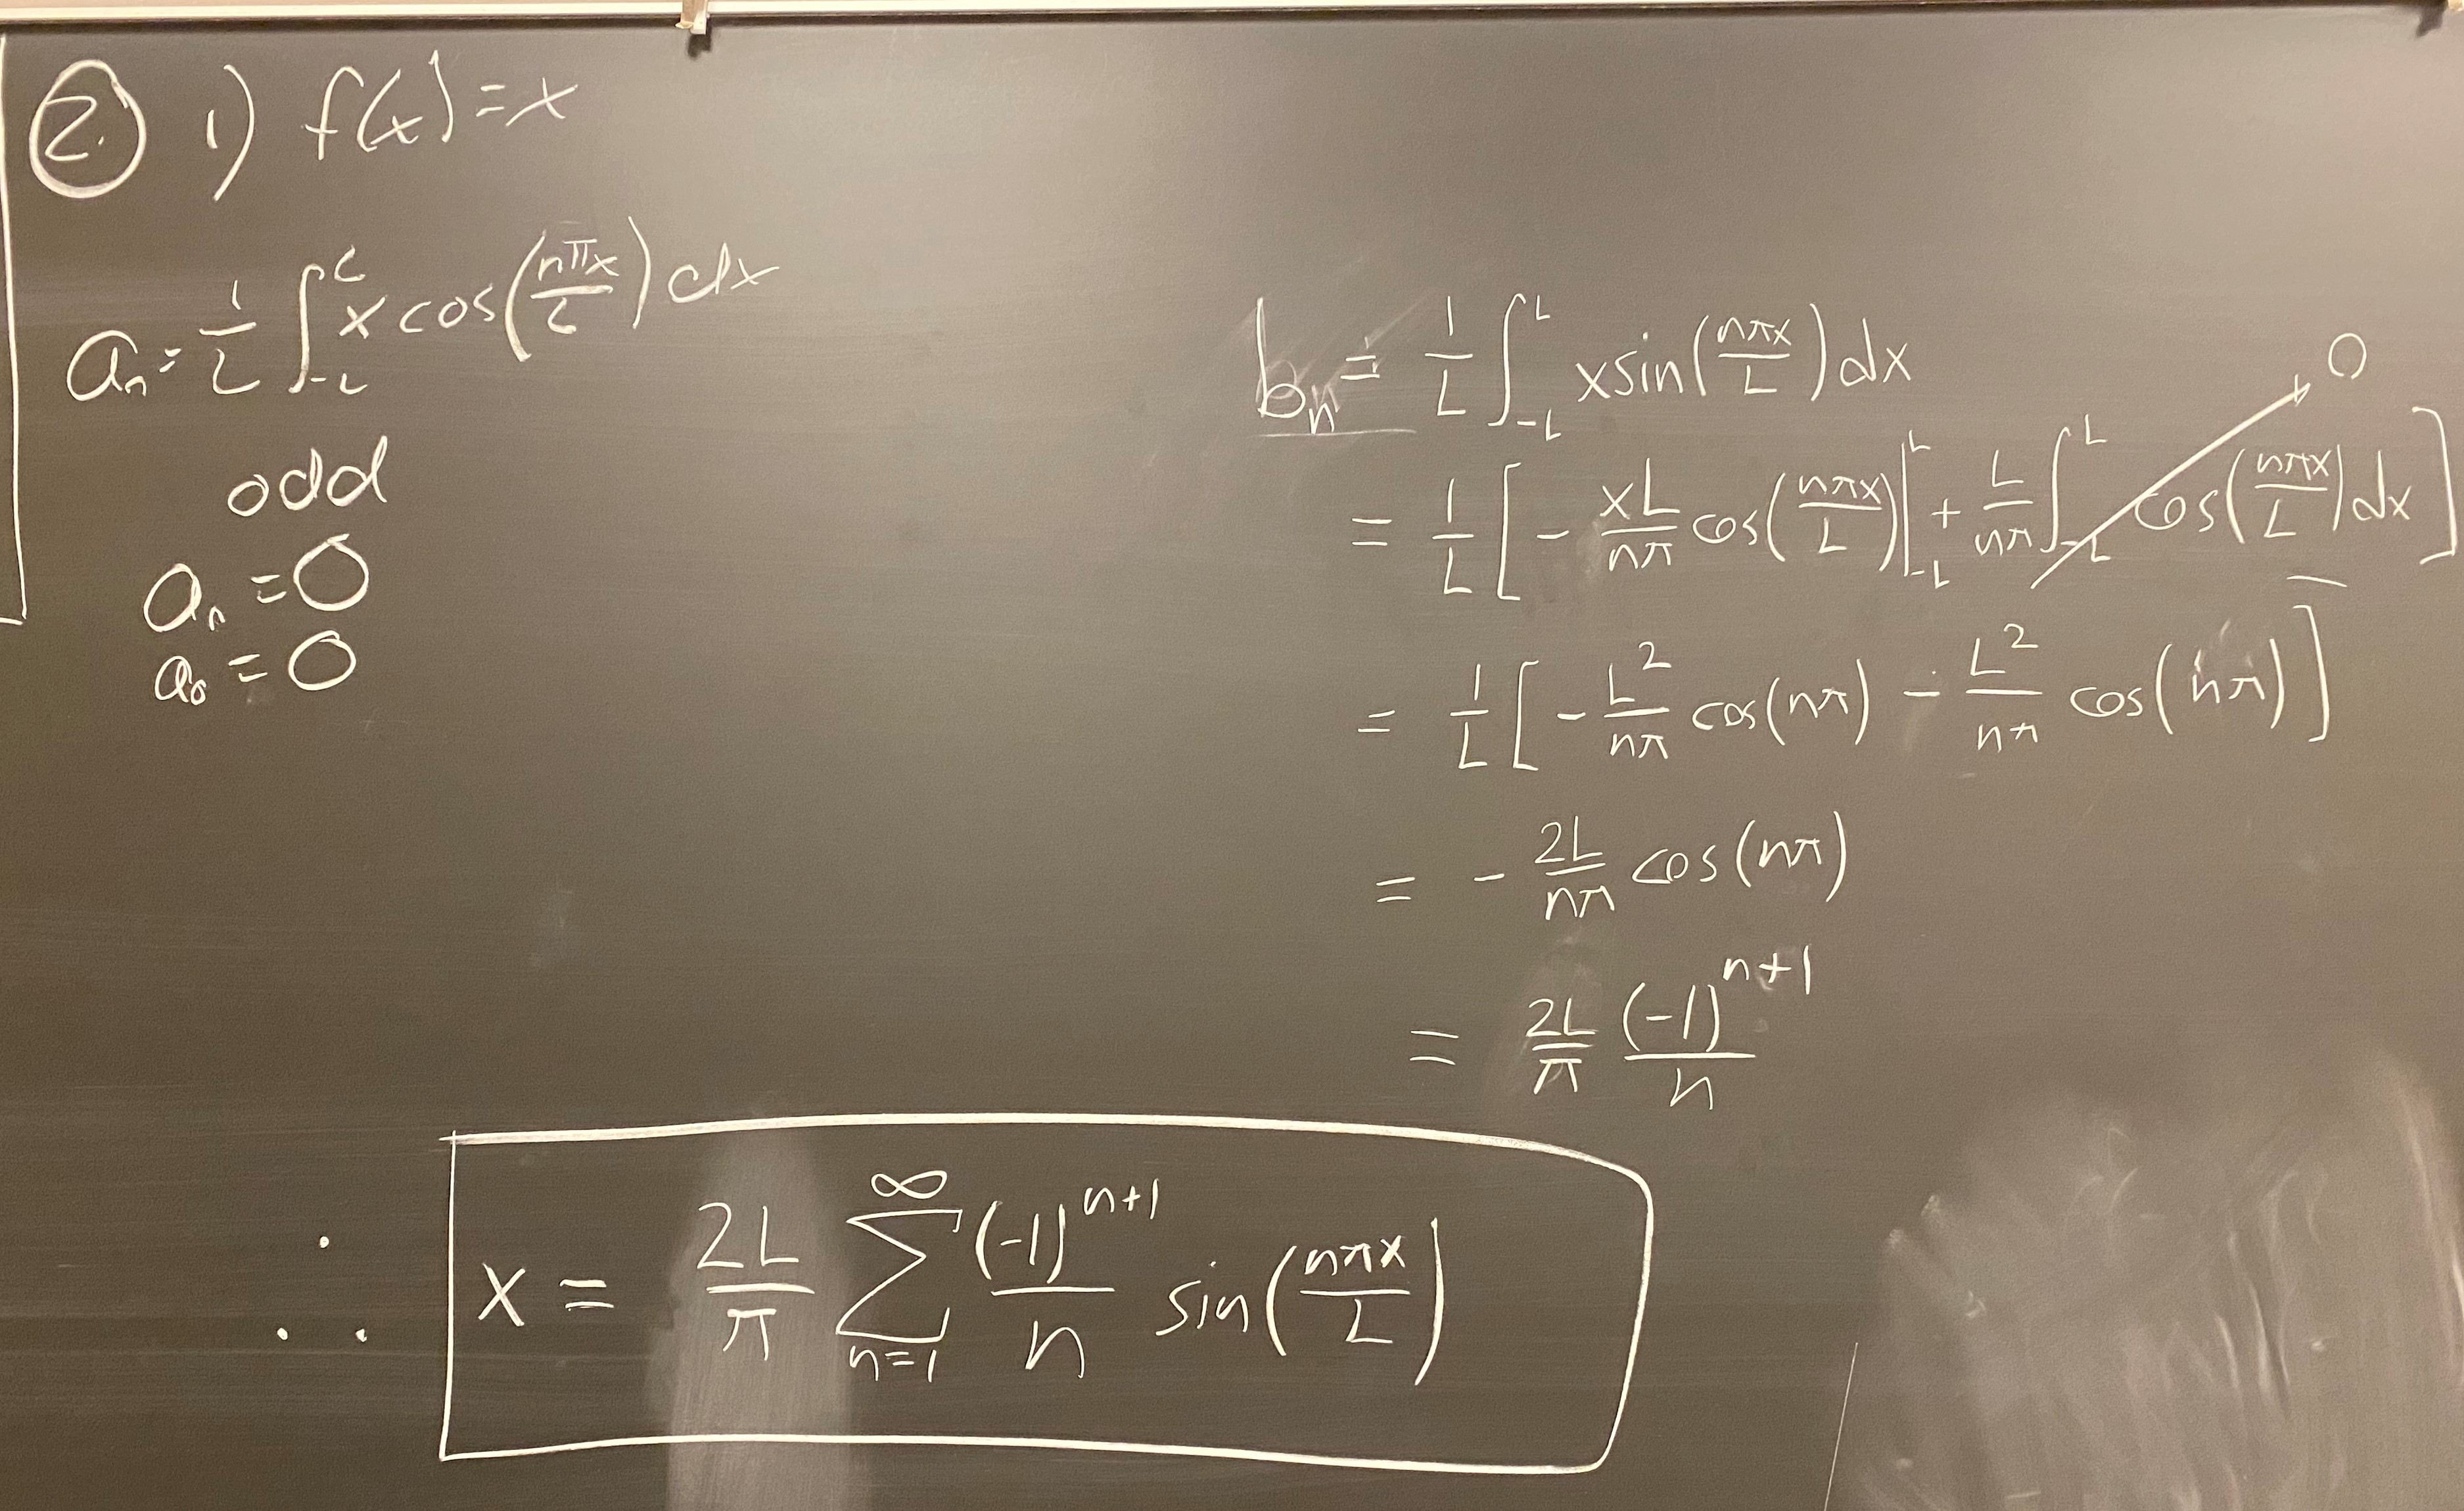
\includegraphics[width = 0.7\textwidth]{Problem 2-1.jpg}
        \end{figure}
        \begin{figure}[H]
            \centering
            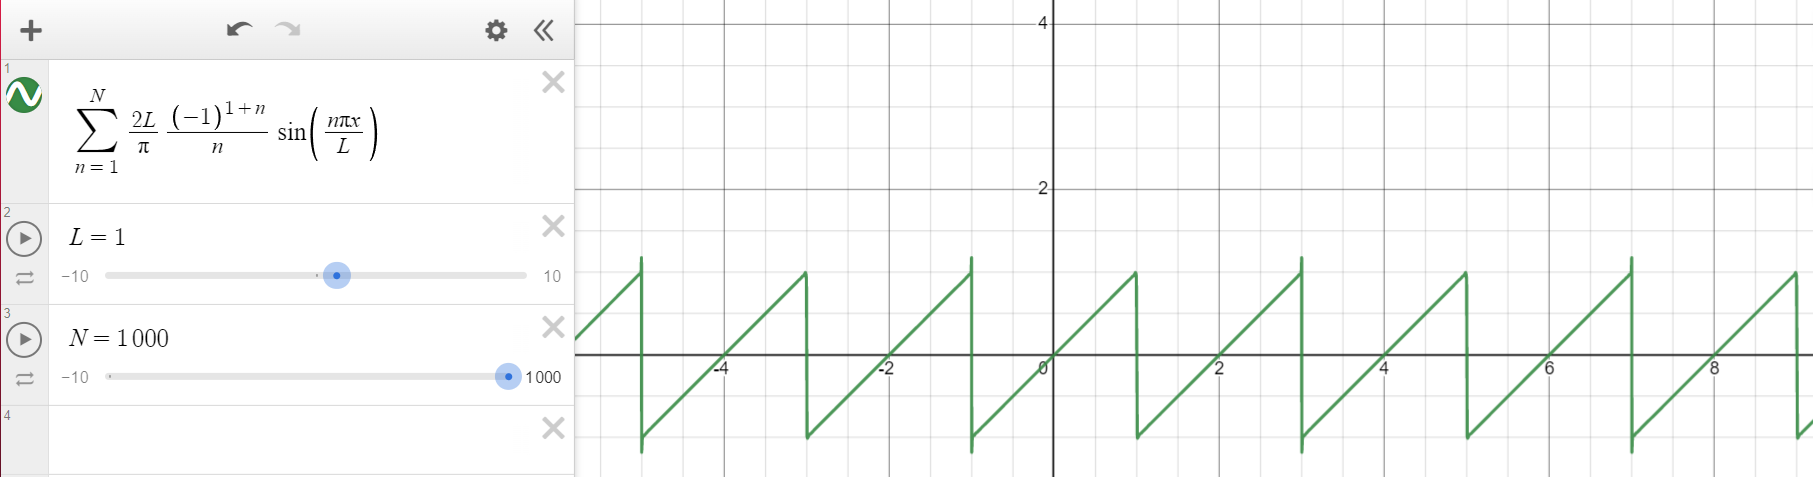
\includegraphics[width = \textwidth]{Problem 2.1.png}
        \end{figure}

        \item \phantom{.}
        \begin{figure}[H]
            \centering
            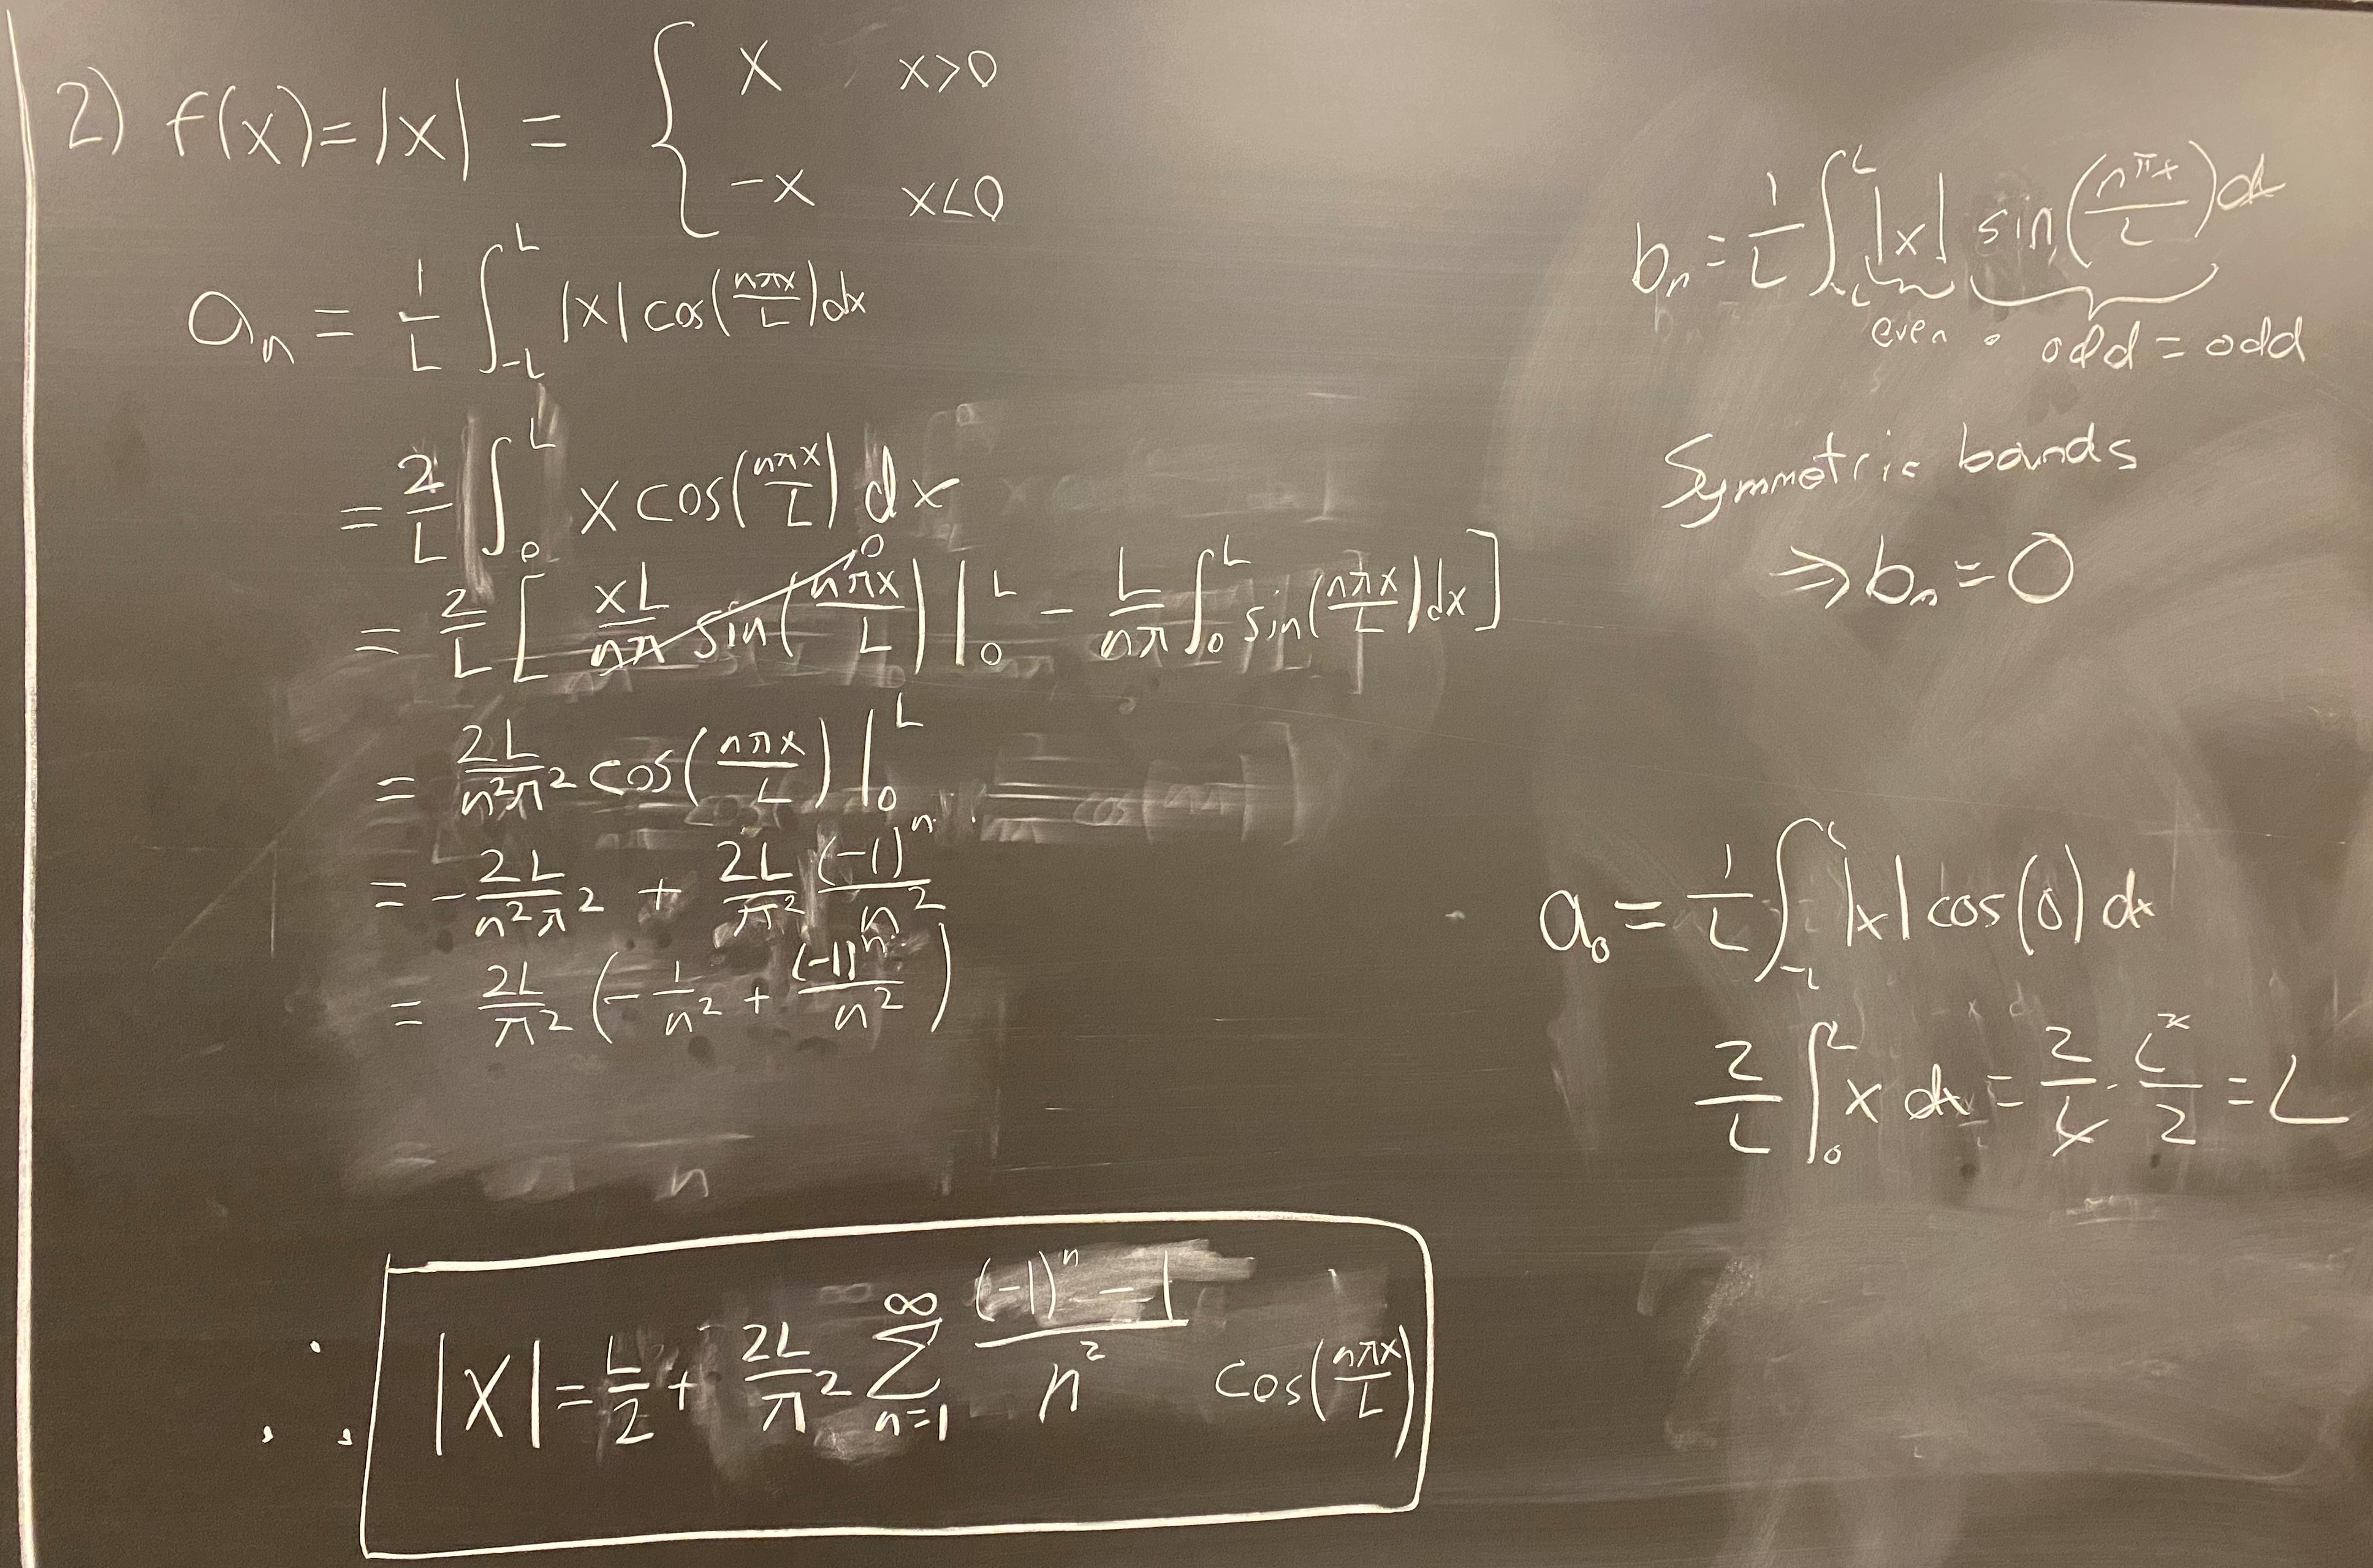
\includegraphics[width = \textwidth]{Problem 2-2.jpg}
            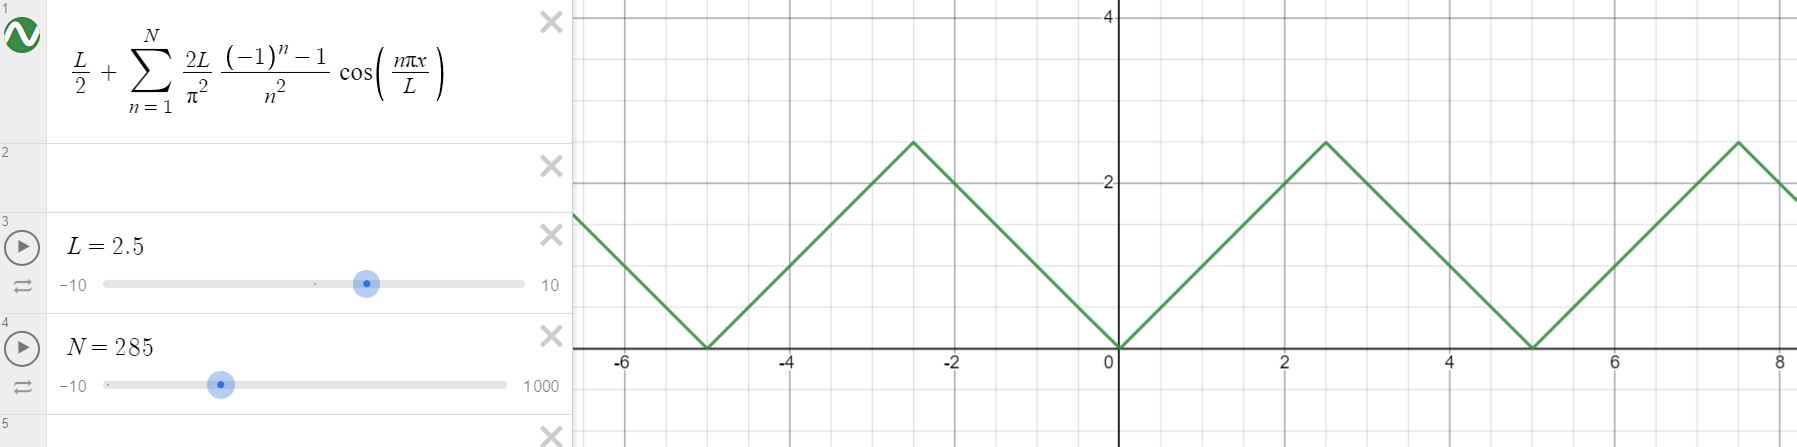
\includegraphics[width = \textwidth]{Problem 2.2.png}
        \end{figure}
\newpage
        \item \phantom{.}
        \begin{figure}[H]
            \centering
            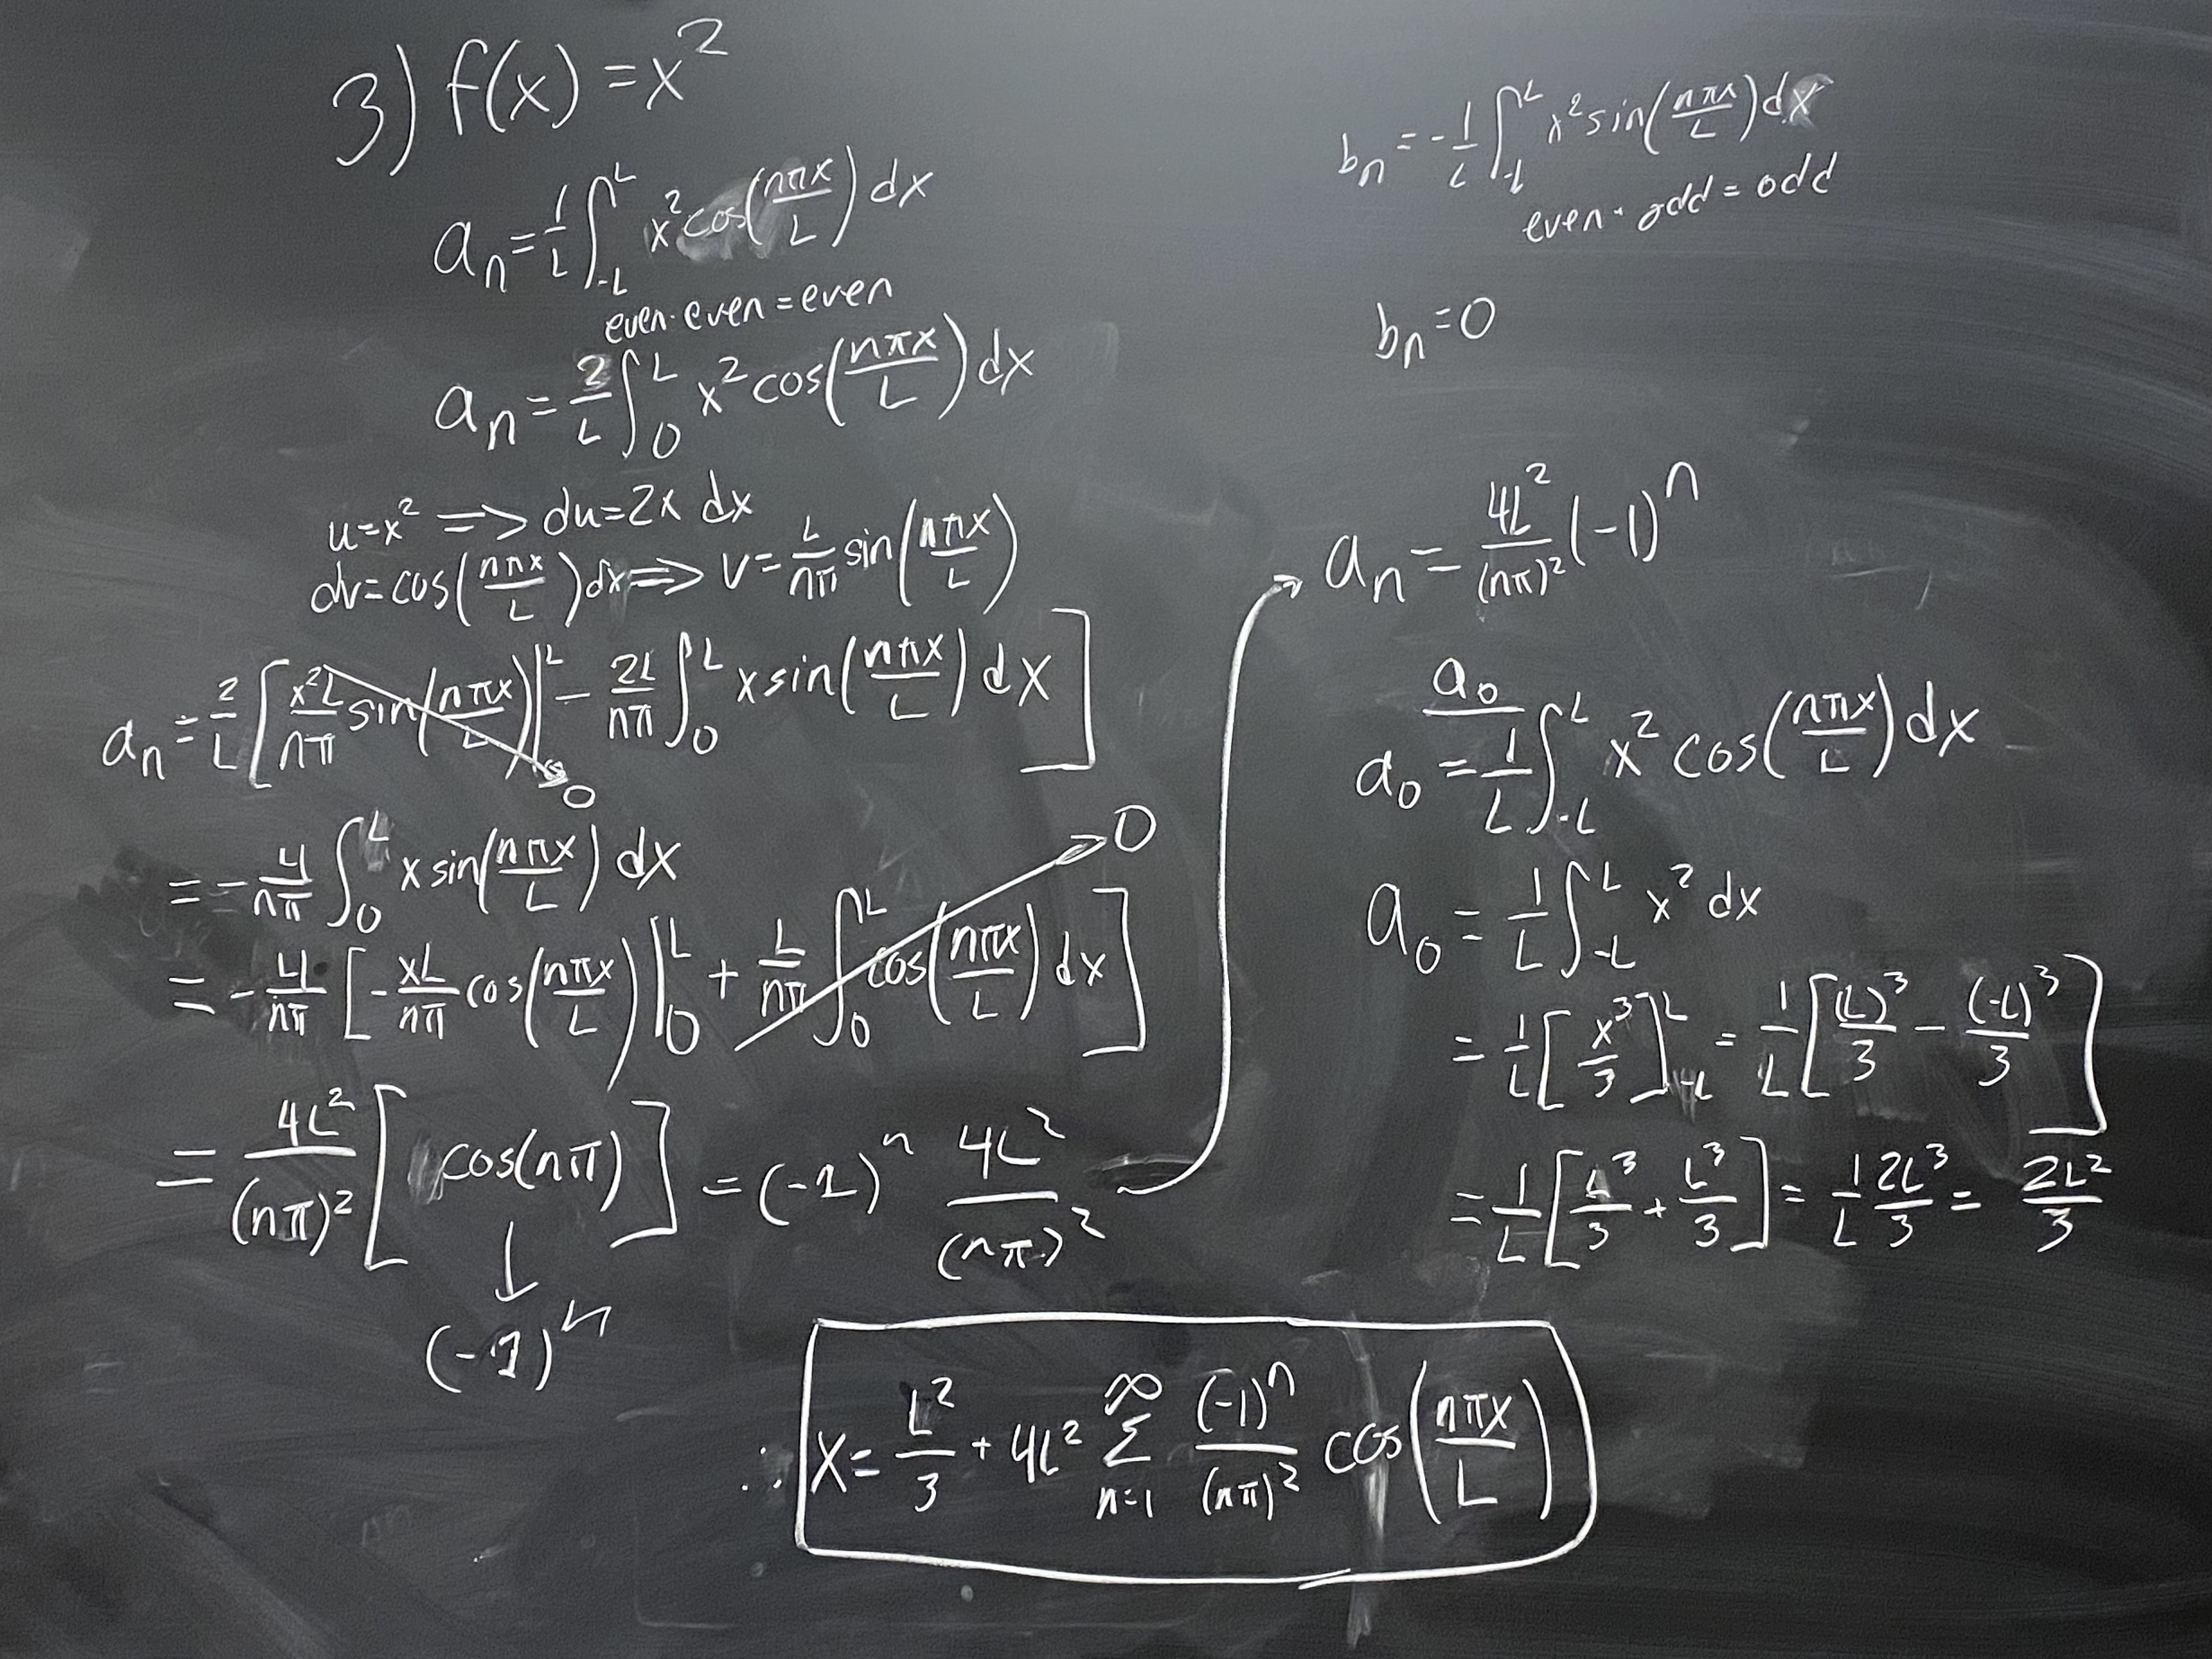
\includegraphics[width = \textwidth]{Problem 2-3.jpg}
            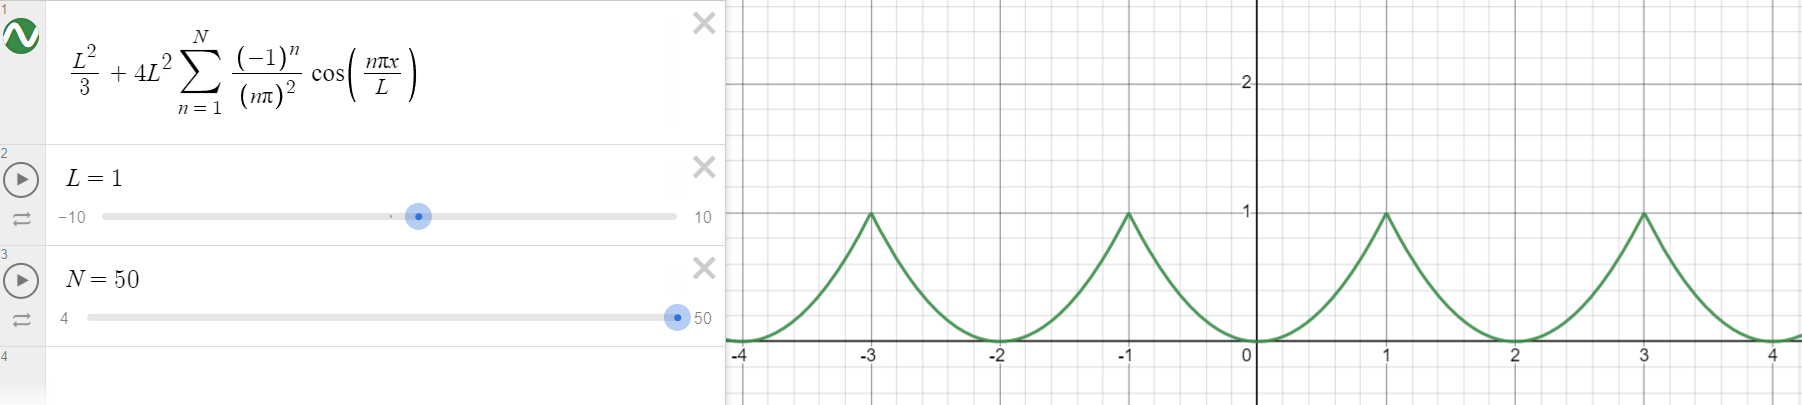
\includegraphics[width = \textwidth]{Problem 2.3.png}
        \end{figure}
    \end{enumerate}
\end{ans}

\begin{boldenv}
    \underline{Problem 3}. Decompose into full Fourier series on interval $[-\pi, \pi]$ and sketch the graph of the sum of such Fourier series: \begin{align}
        & |\sin(x)|\\
        & |\cos(x)|
    \end{align}
\end{boldenv}
\newpage
\begin{ans}
    \begin{enumerate}
        \item \phantom{.}
        \begin{figure}[H]
            \centering
            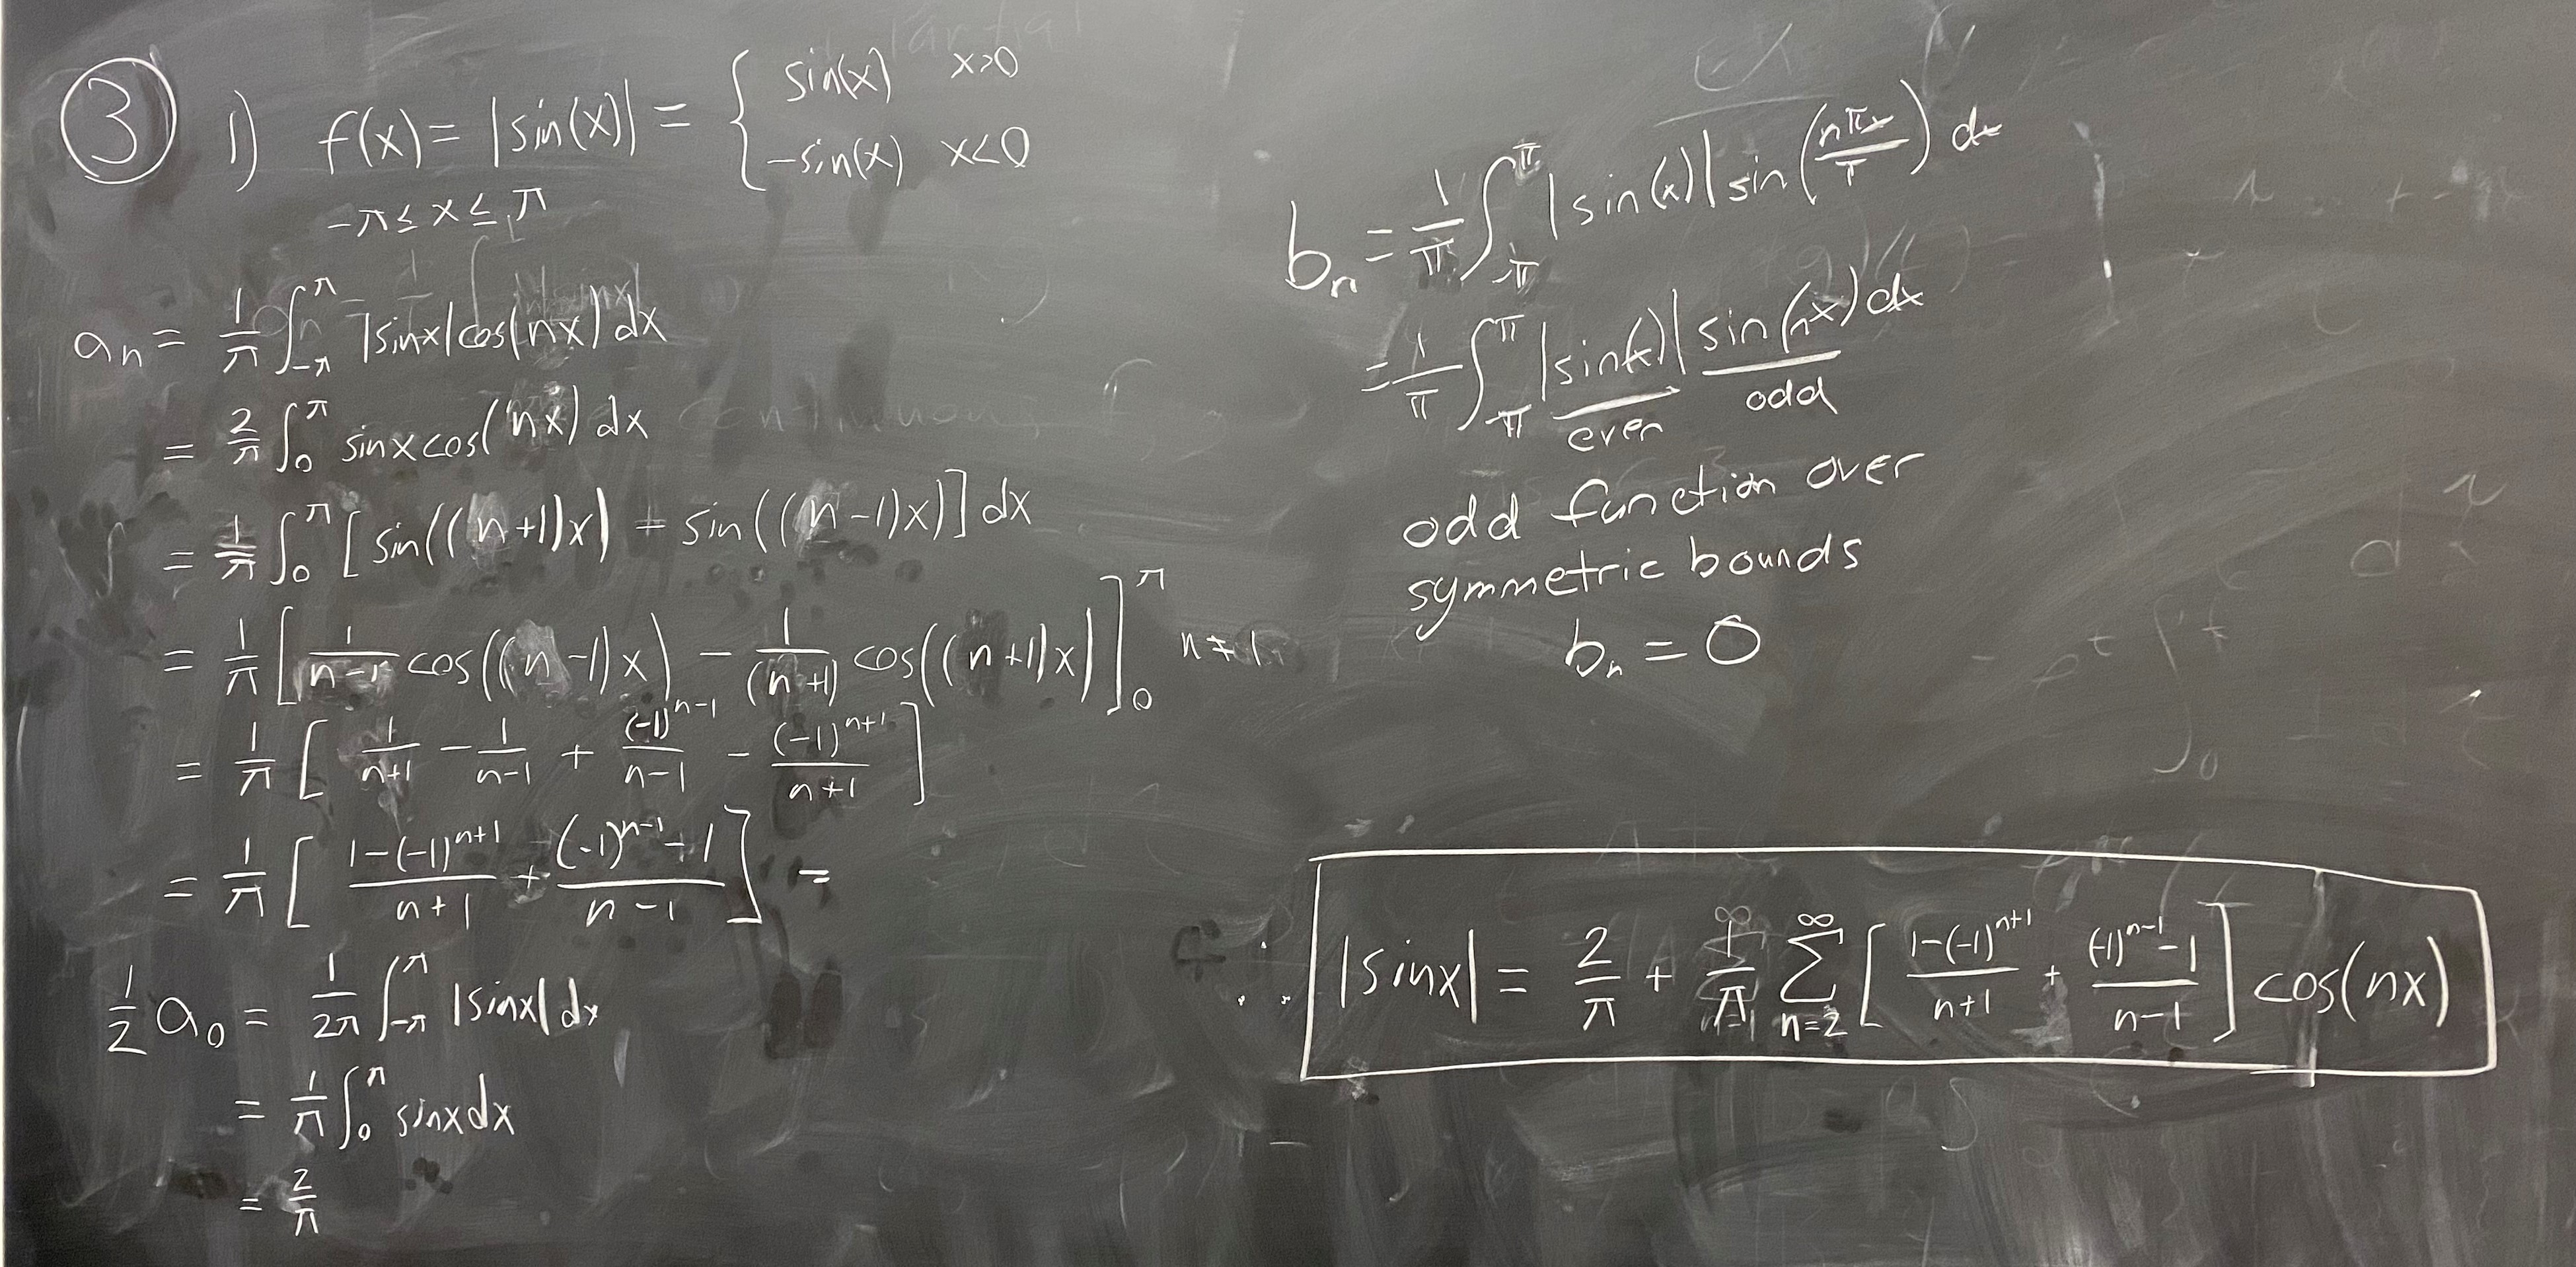
\includegraphics[width = .8\textwidth]{Problem 3-1.png}
            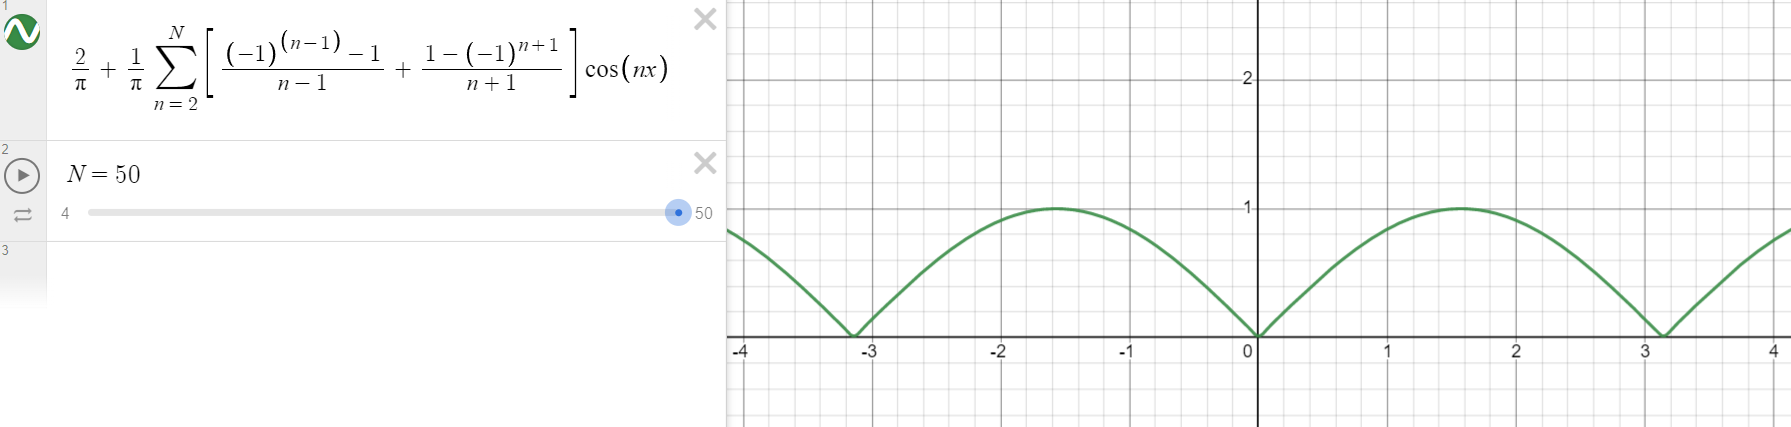
\includegraphics[width = .8\textwidth]{Problem 3.1.png}
        \end{figure}

        \item \phantom{.}
        \begin{figure}[H]
            \centering
            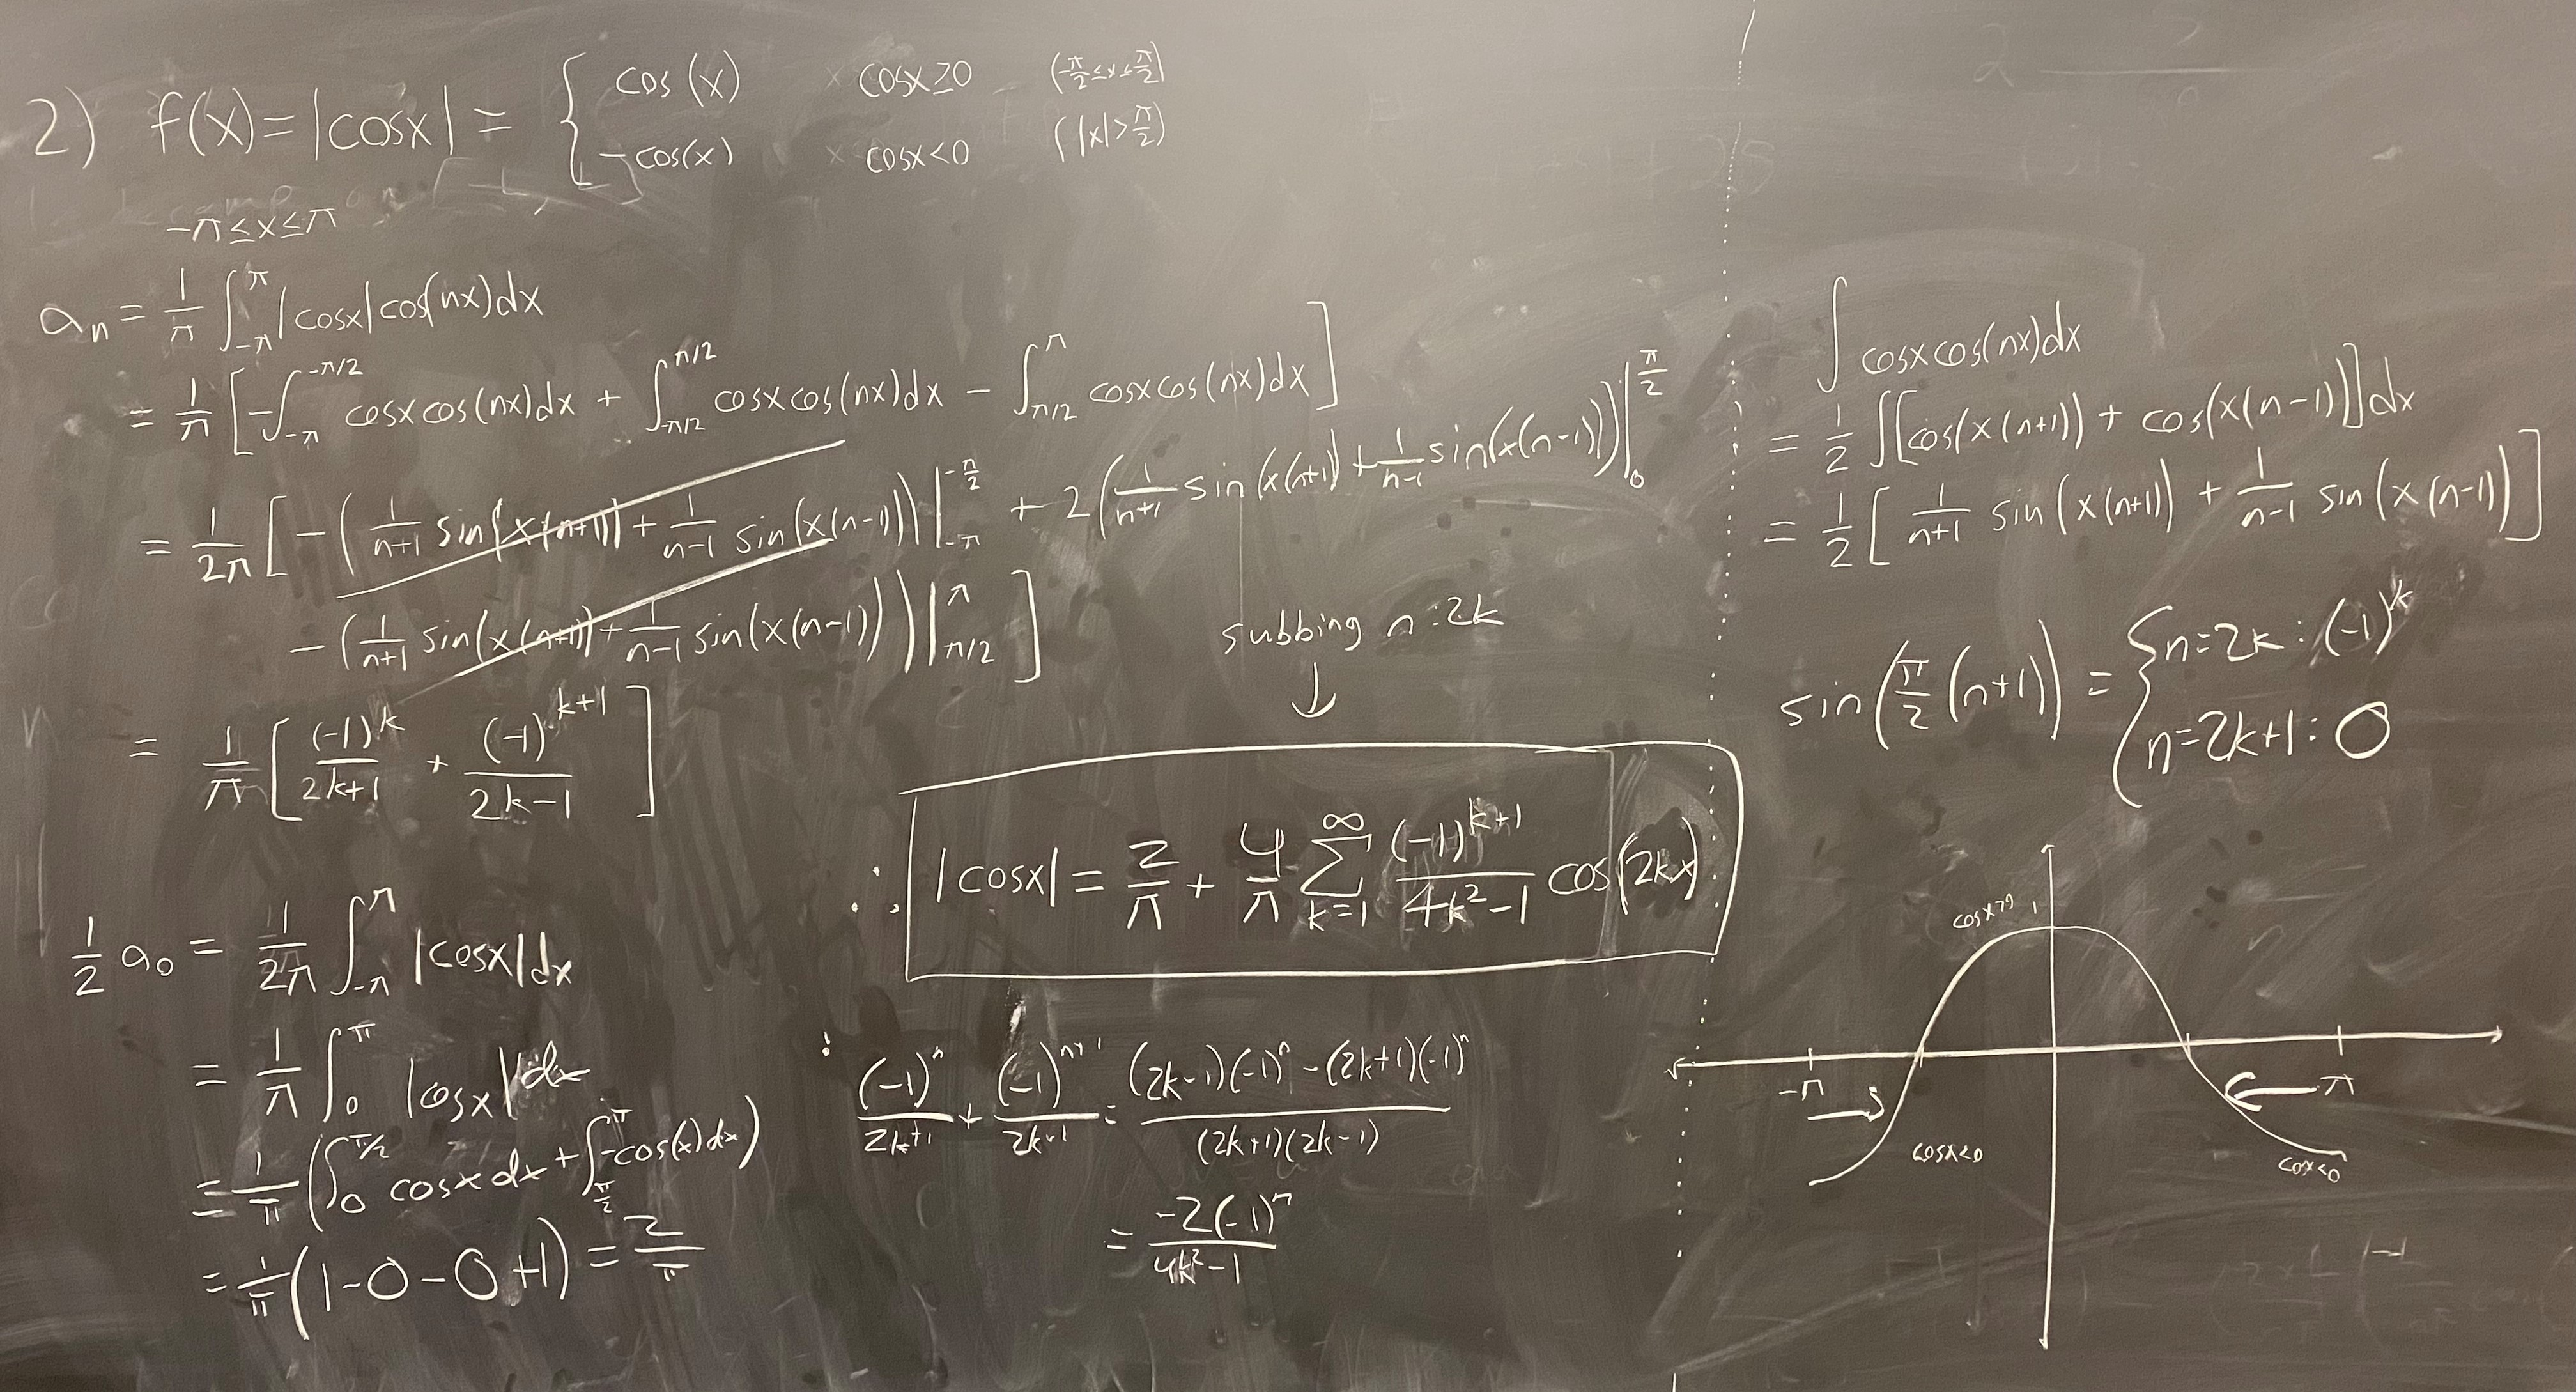
\includegraphics[width = .8\textwidth]{Problem 3-2.png}
            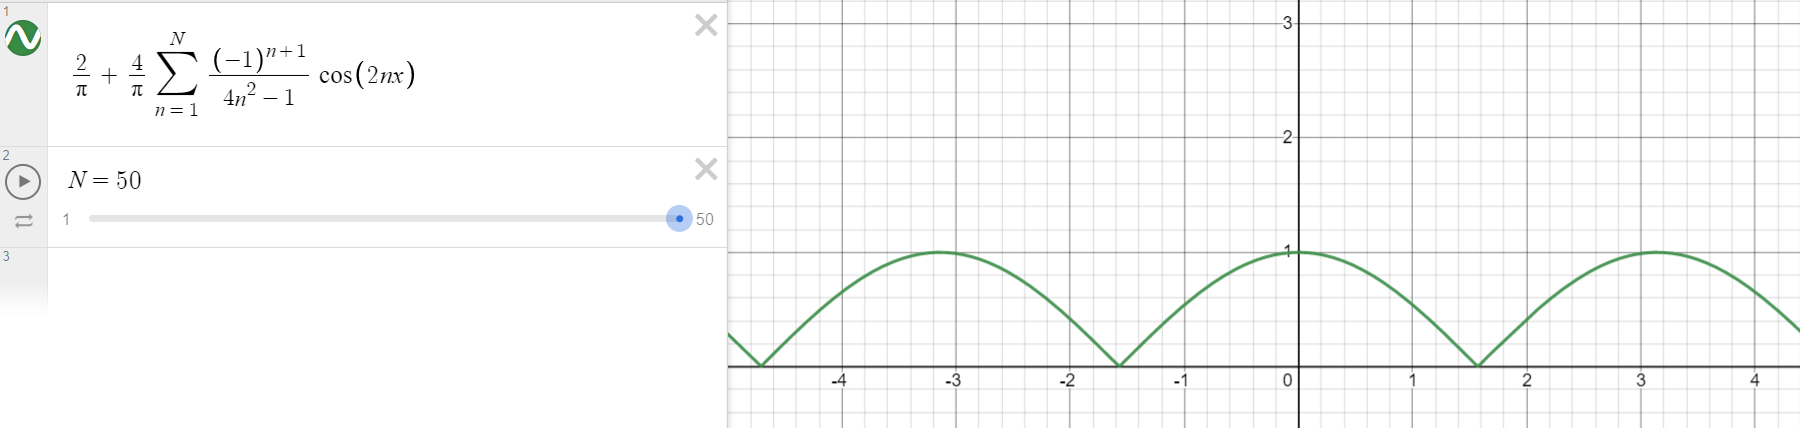
\includegraphics[width = .8\textwidth]{Problem 3.2.png}
        \end{figure}
    \end{enumerate}
\end{ans}

\begin{boldenv}
    \underline{Problem 4}. Decompose into sin-Fourier series on interval $[0, \pi]$ and sketch the graph of the sum of such Fourier series: \begin{align}
        & 1\\
        & x\\
        & x(\pi - x)\\
        & \sin(mx) \text{ with } m \in \N\\
        & \cos(mx) \text{ with } m \in \N\\
        & \sin((m - \frac{1}{2})x) \text{ with } m \in \N
    \end{align}
\end{boldenv}
\begin{ans}
    \begin{enumerate}
        \item \phantom{.}\begin{figure}[H]
            \centering
            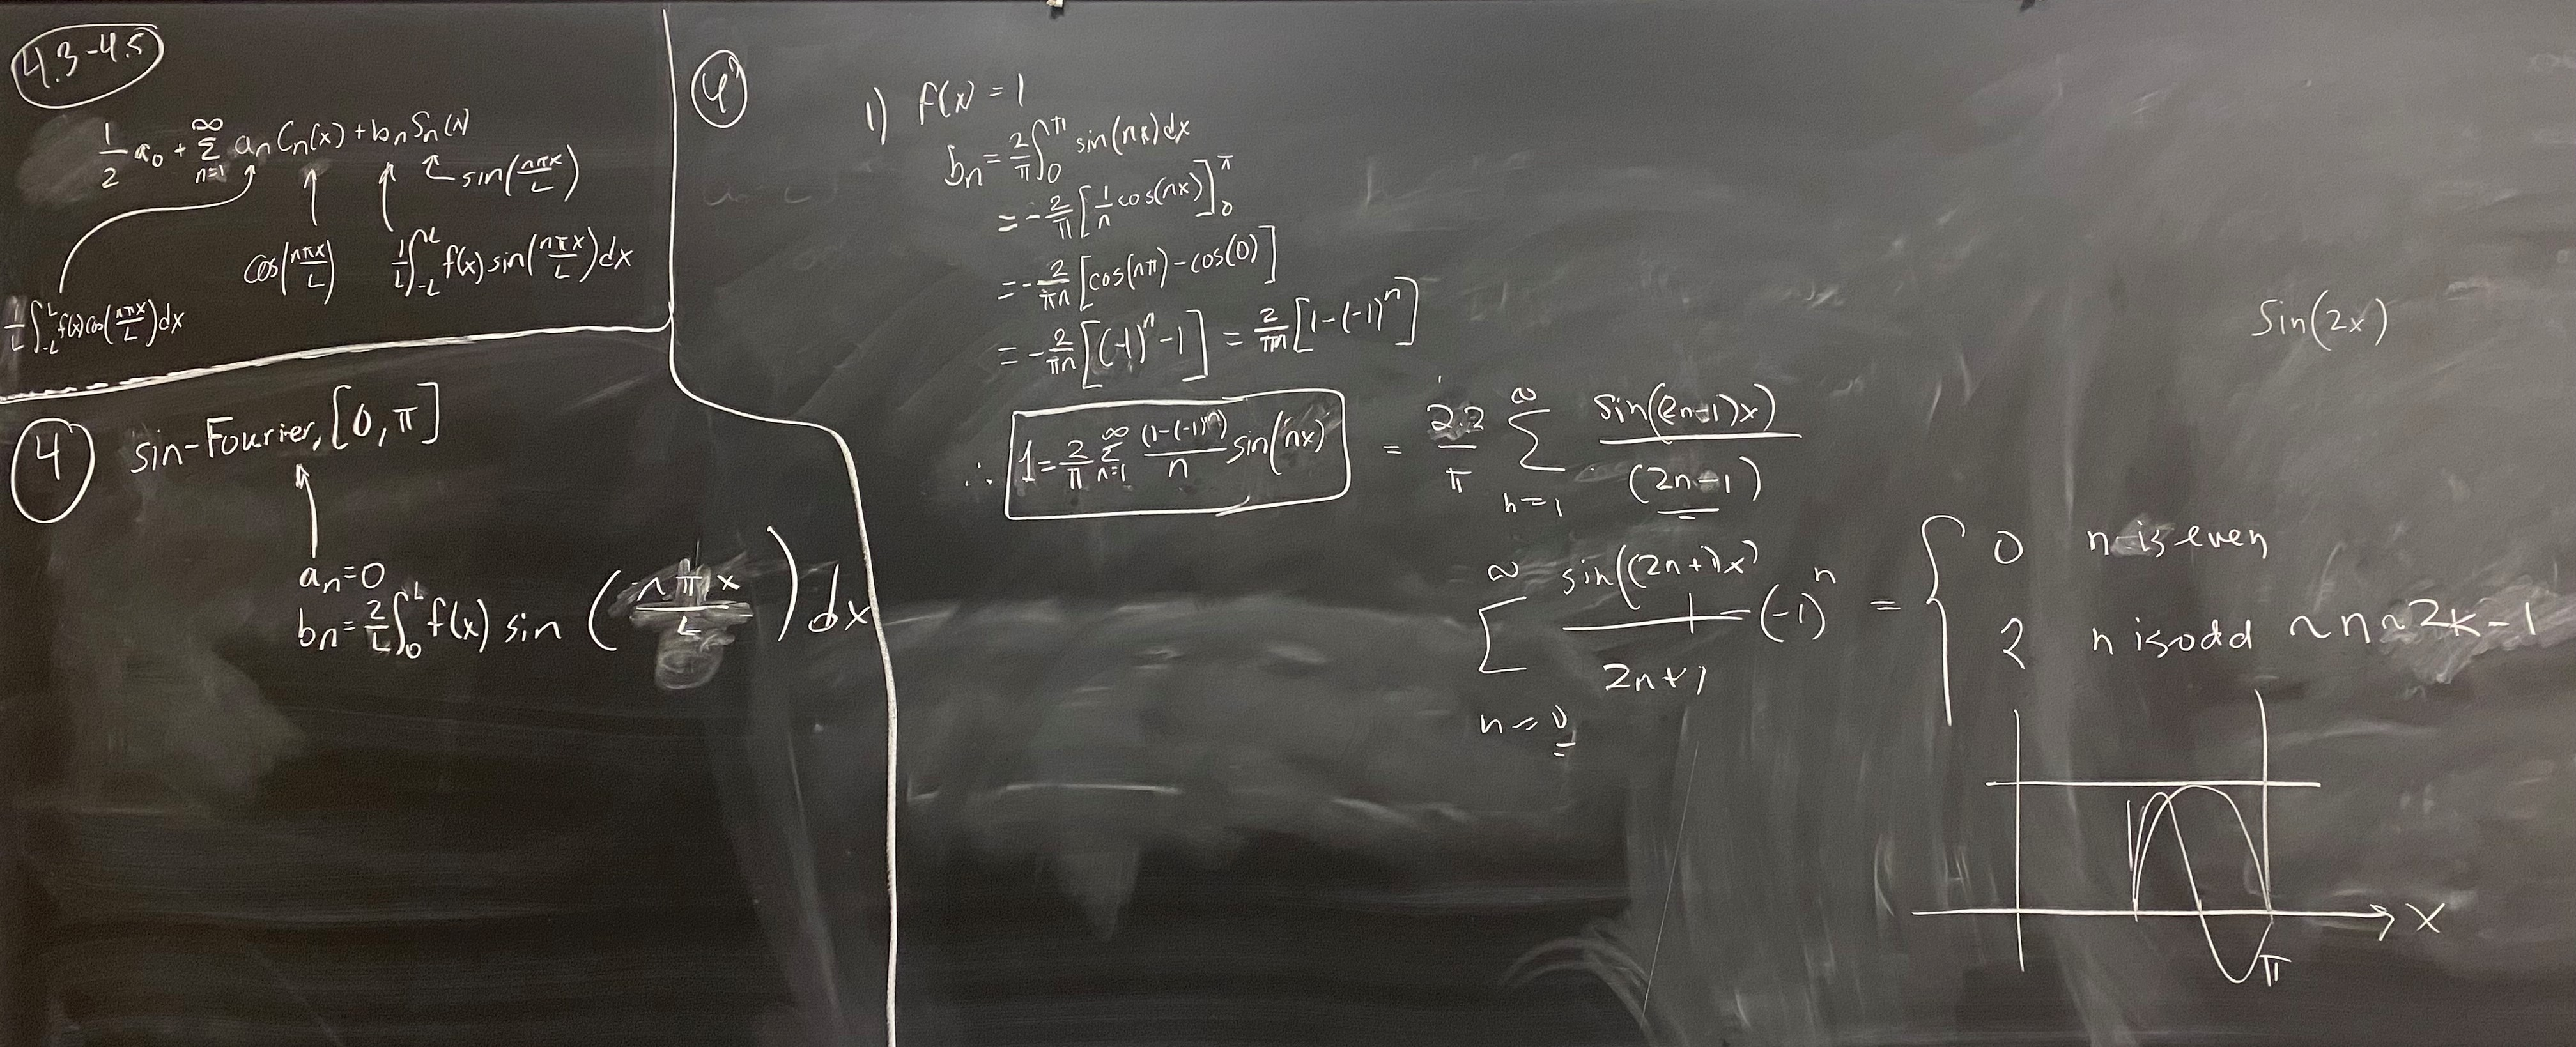
\includegraphics[width = \textwidth]{Problem 4-1.png}
            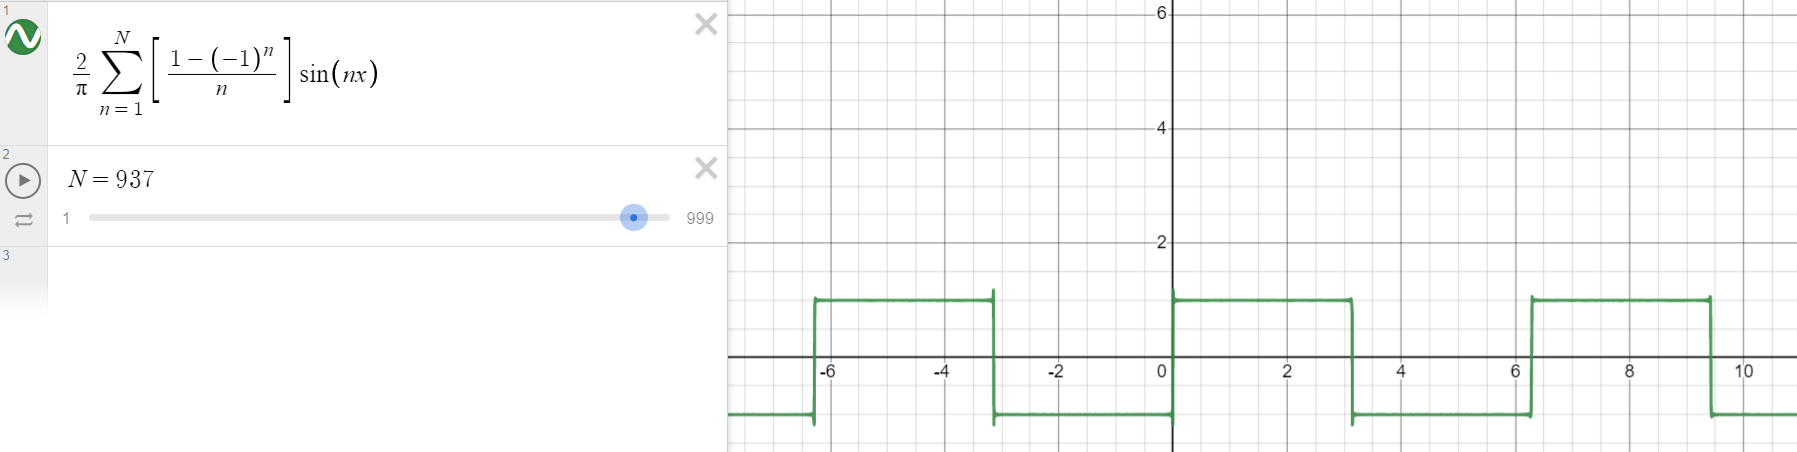
\includegraphics[width = \textwidth]{Problem 4.1.png}
        \end{figure}
\newpage
        \item \phantom{.}
        \begin{figure}[H]
        \centering
        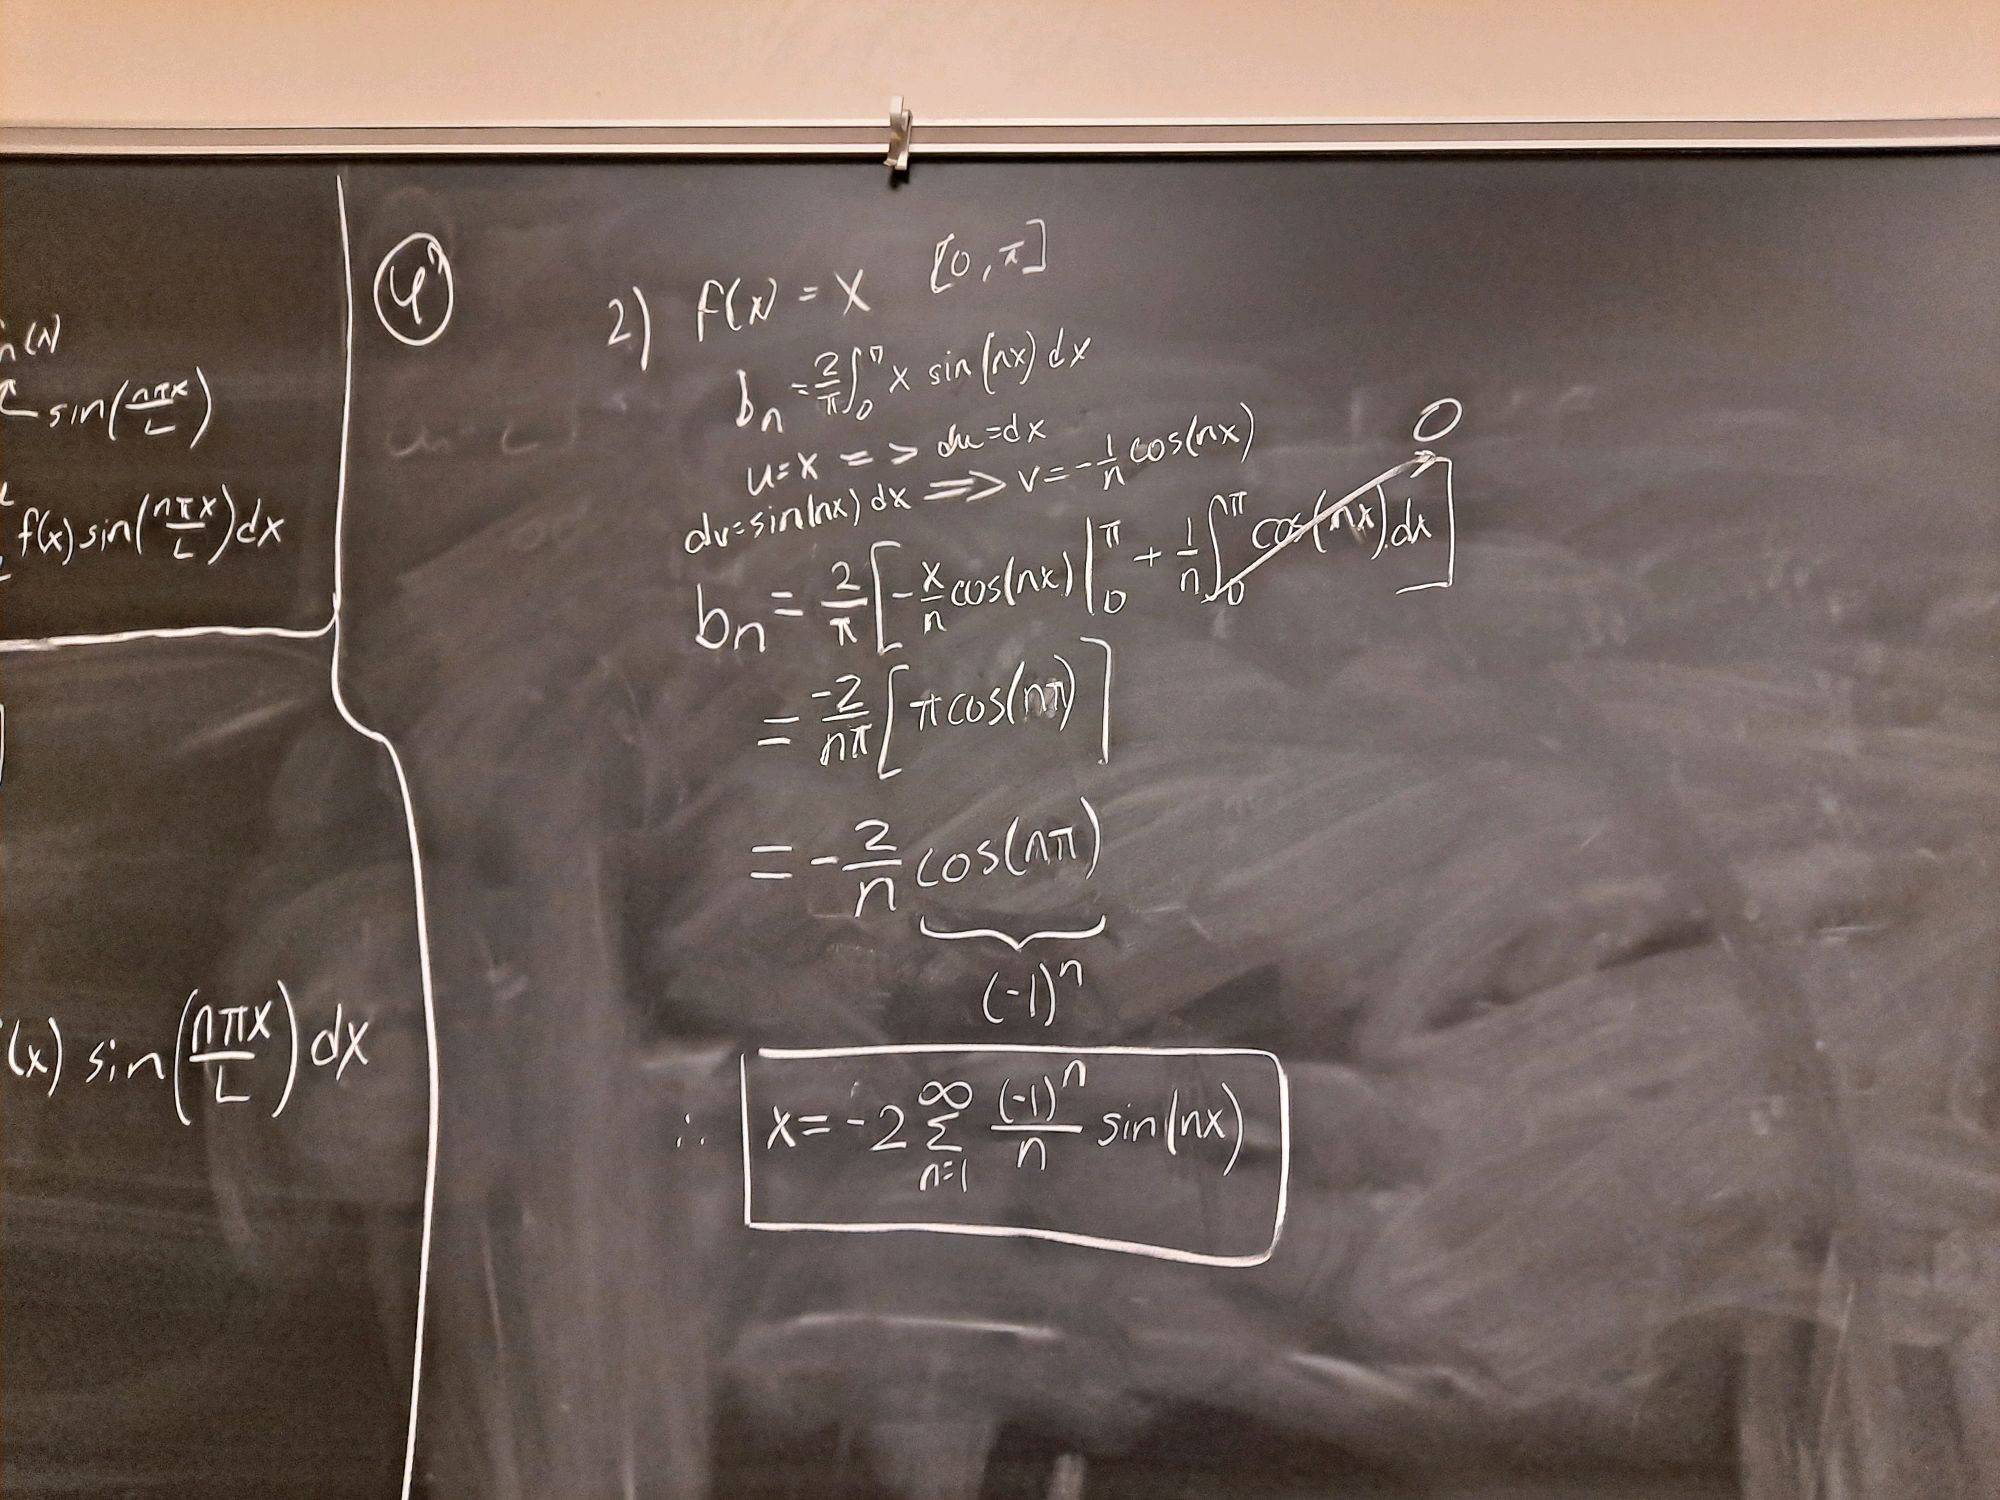
\includegraphics[width = \textwidth]{Problem 4 Part 2.jpeg}
        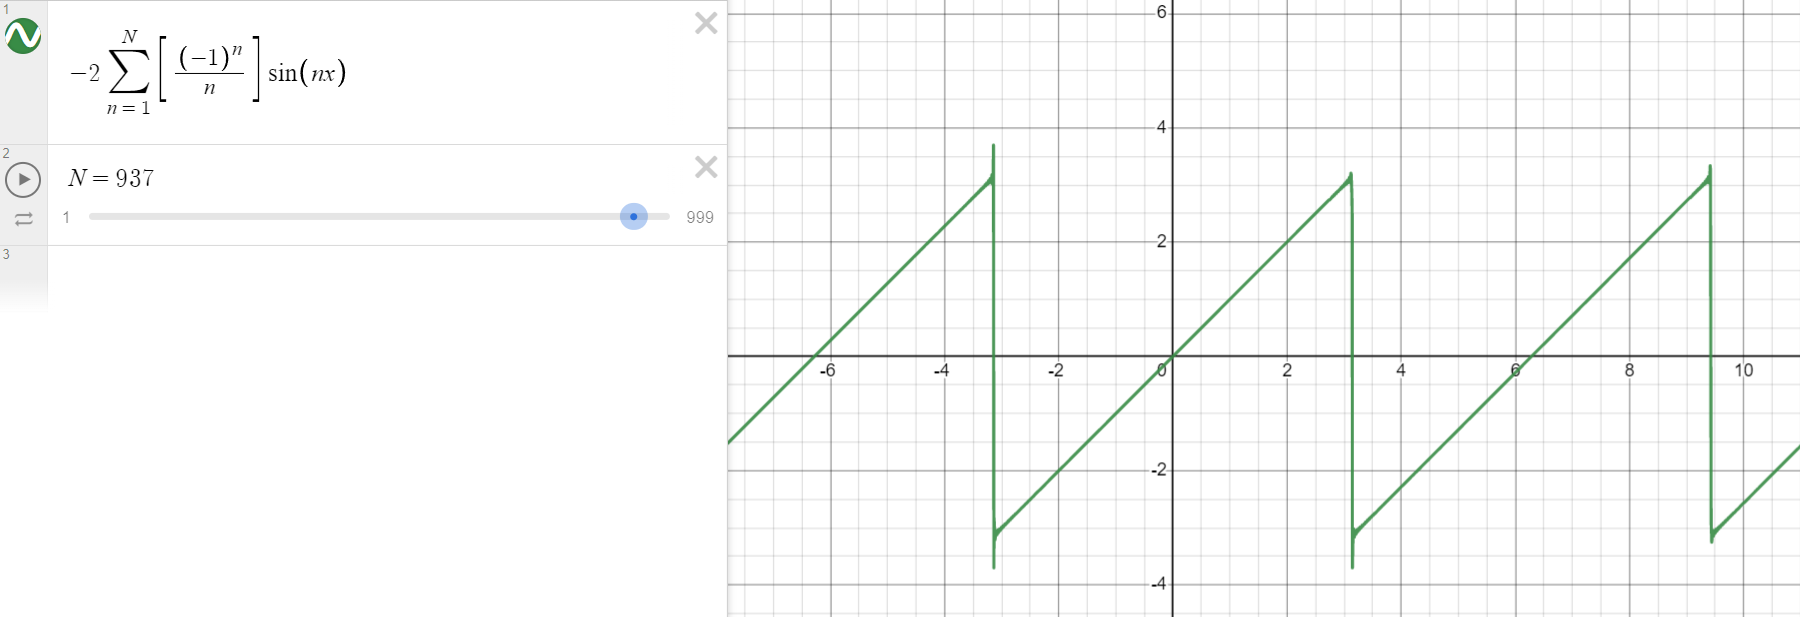
\includegraphics[width = \textwidth]{Problem 4.2.png}
        \end{figure}
\newpage
        \item \phantom{.}
        \begin{figure}[H]
        \centering
        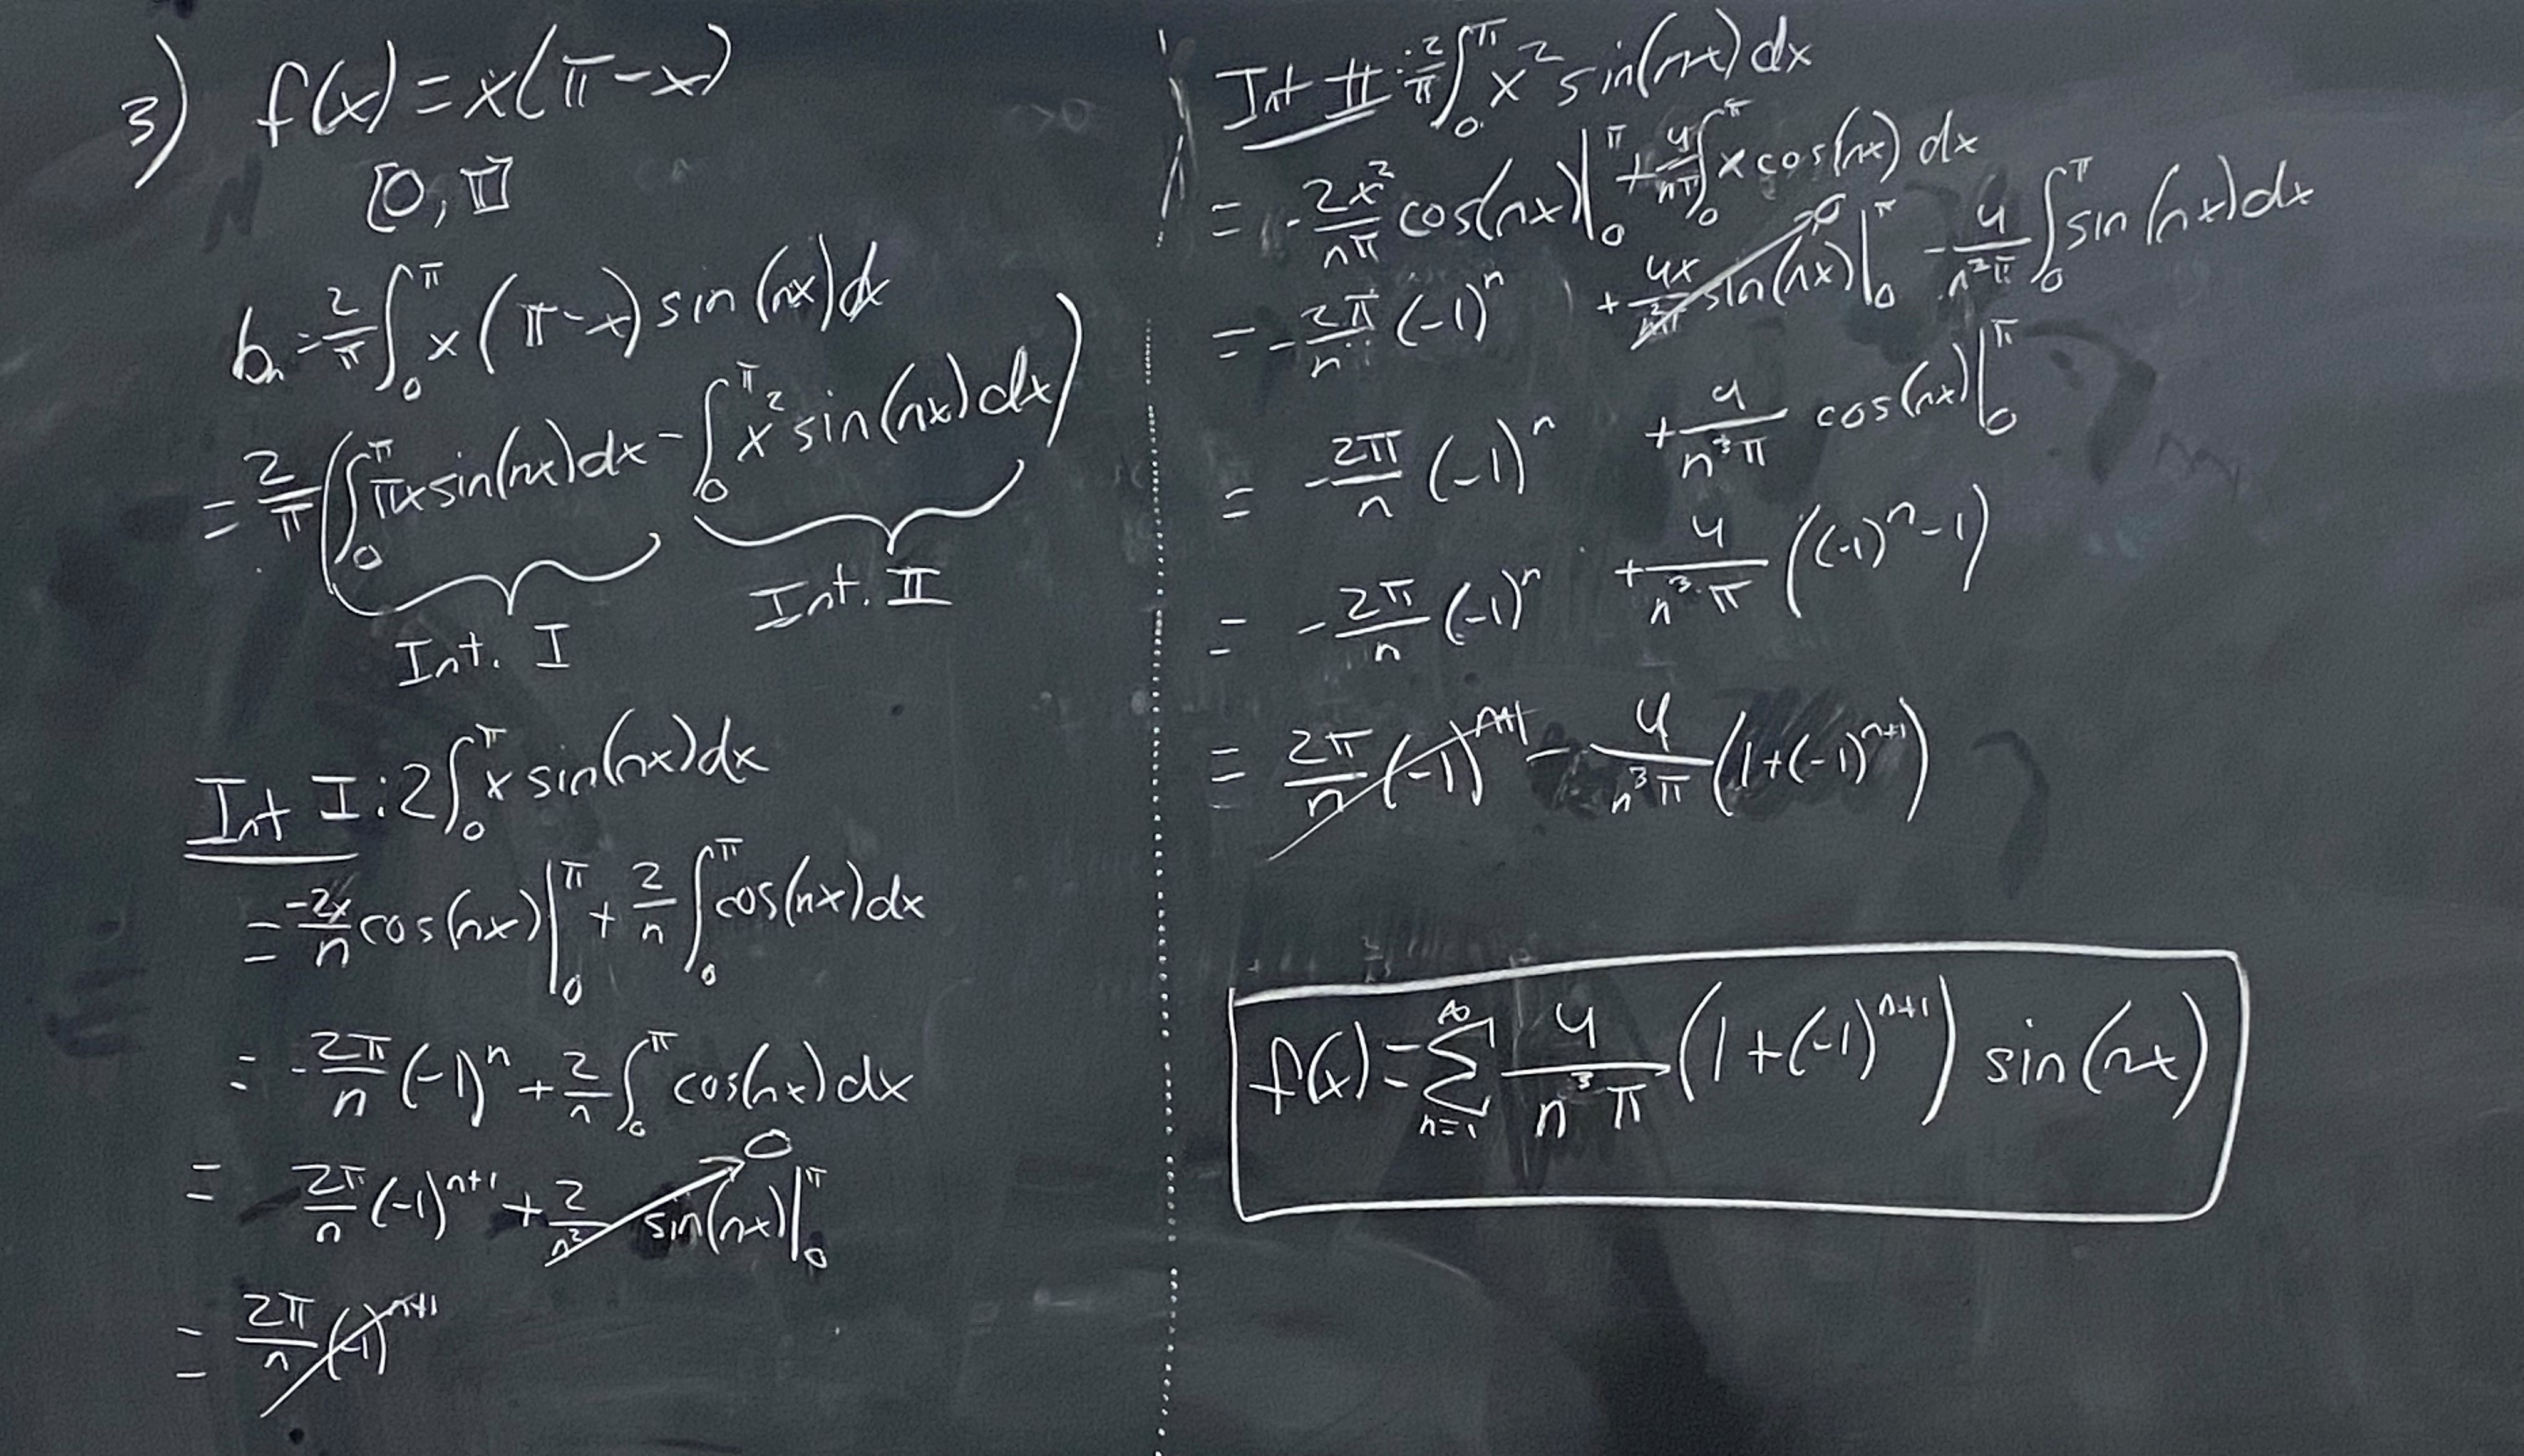
\includegraphics[width = 0.8\textwidth]{Problem 4-3.png}
        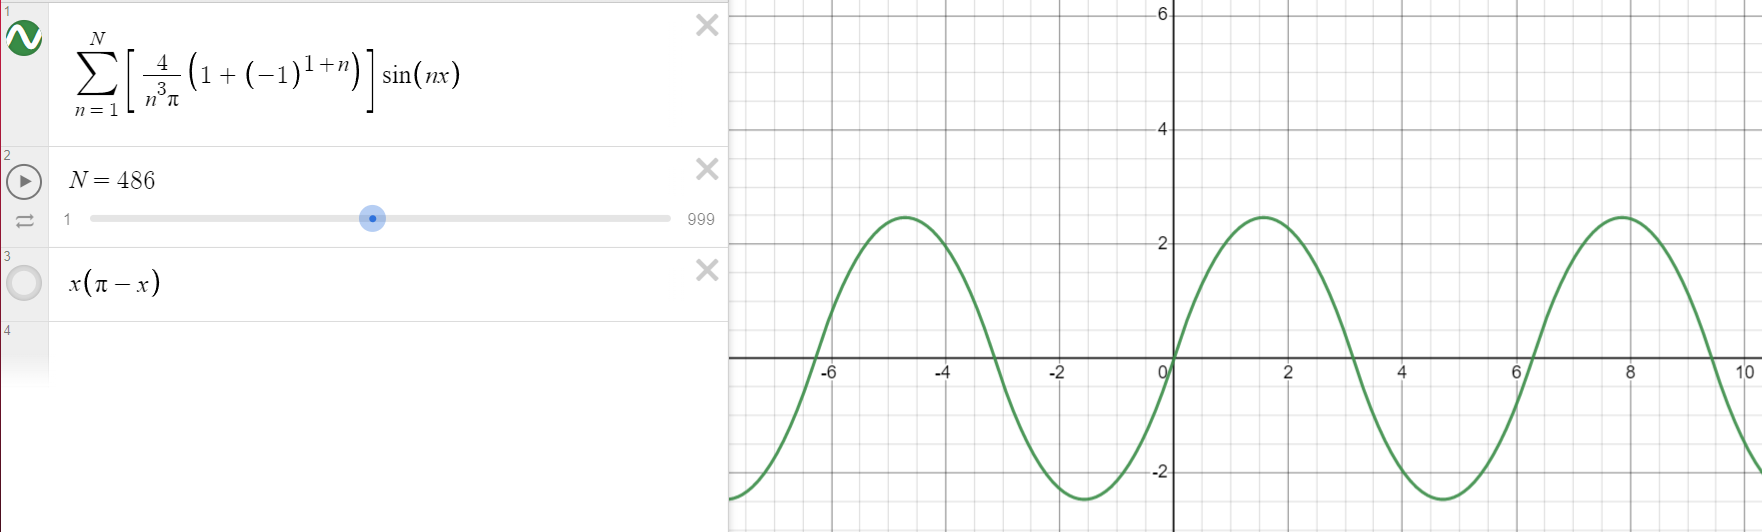
\includegraphics[width = 0.8\textwidth]{Problem 4.3.png}
        \end{figure}

        \item \phantom{.}
        \begin{figure}[H]
        \centering
        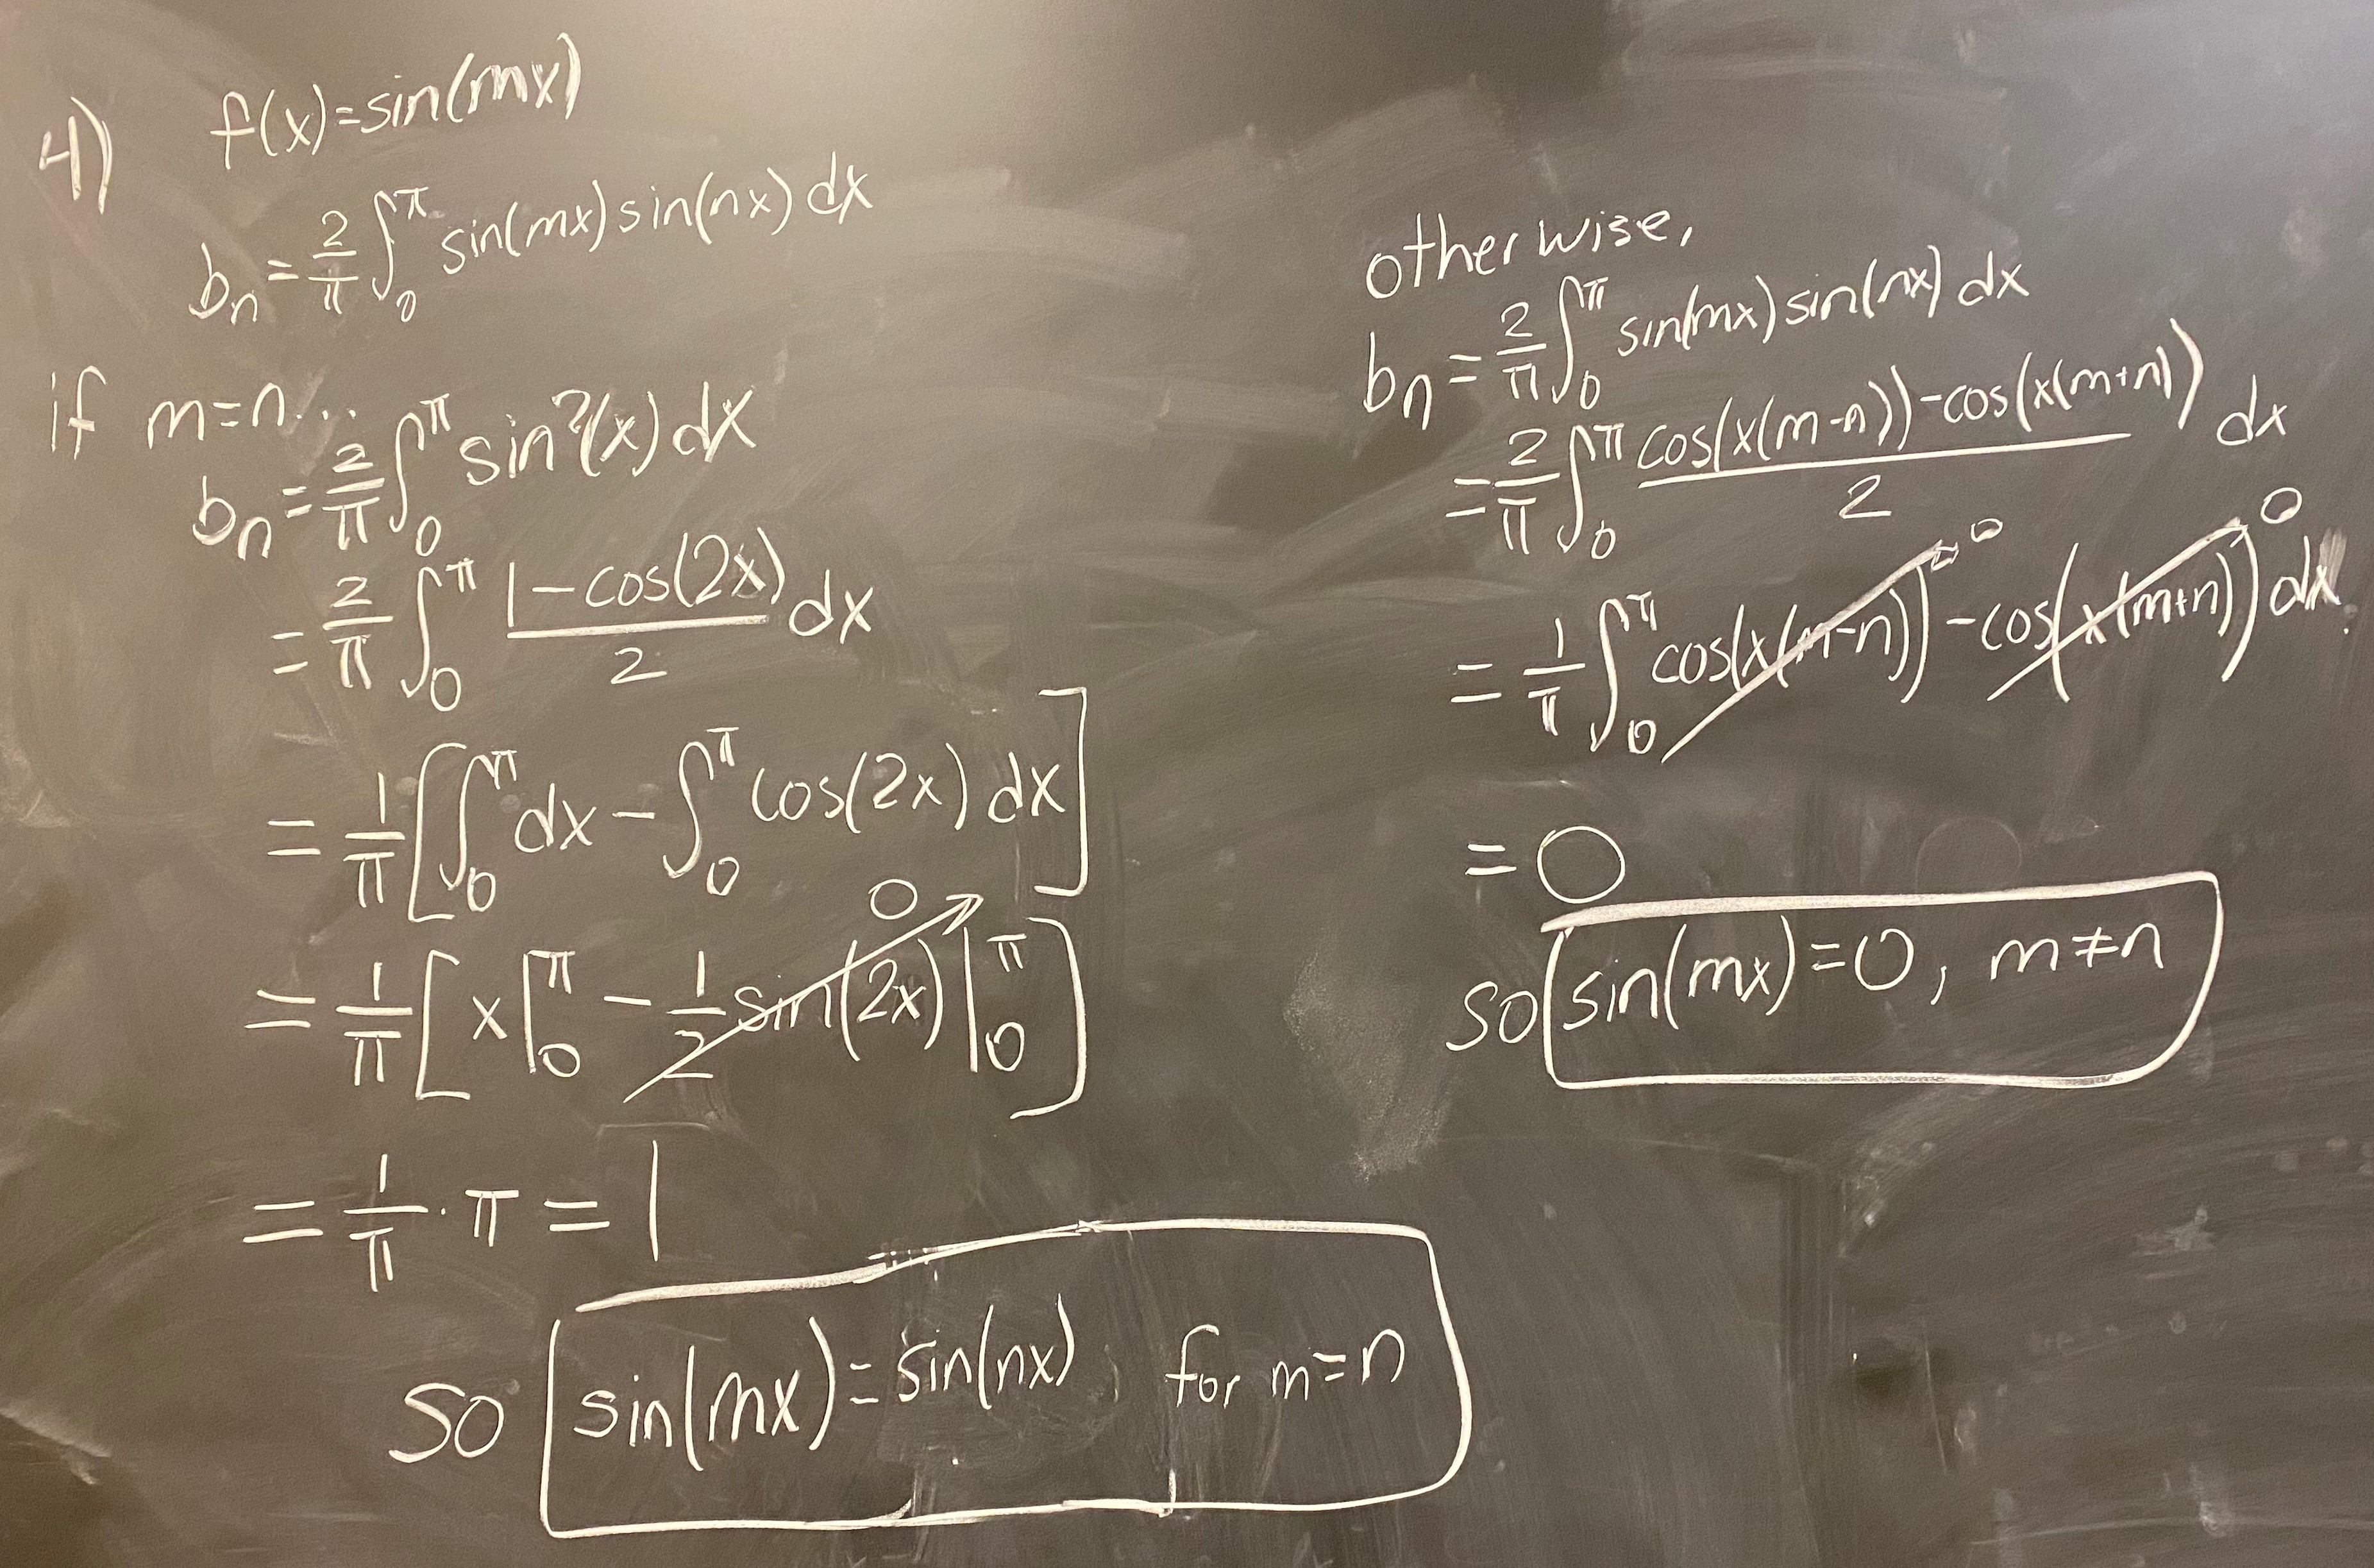
\includegraphics[width = 0.8\textwidth]{Problem 4-4.png}
        \end{figure}

        \item \phantom{.} \begin{figure}[H]
            \centering
            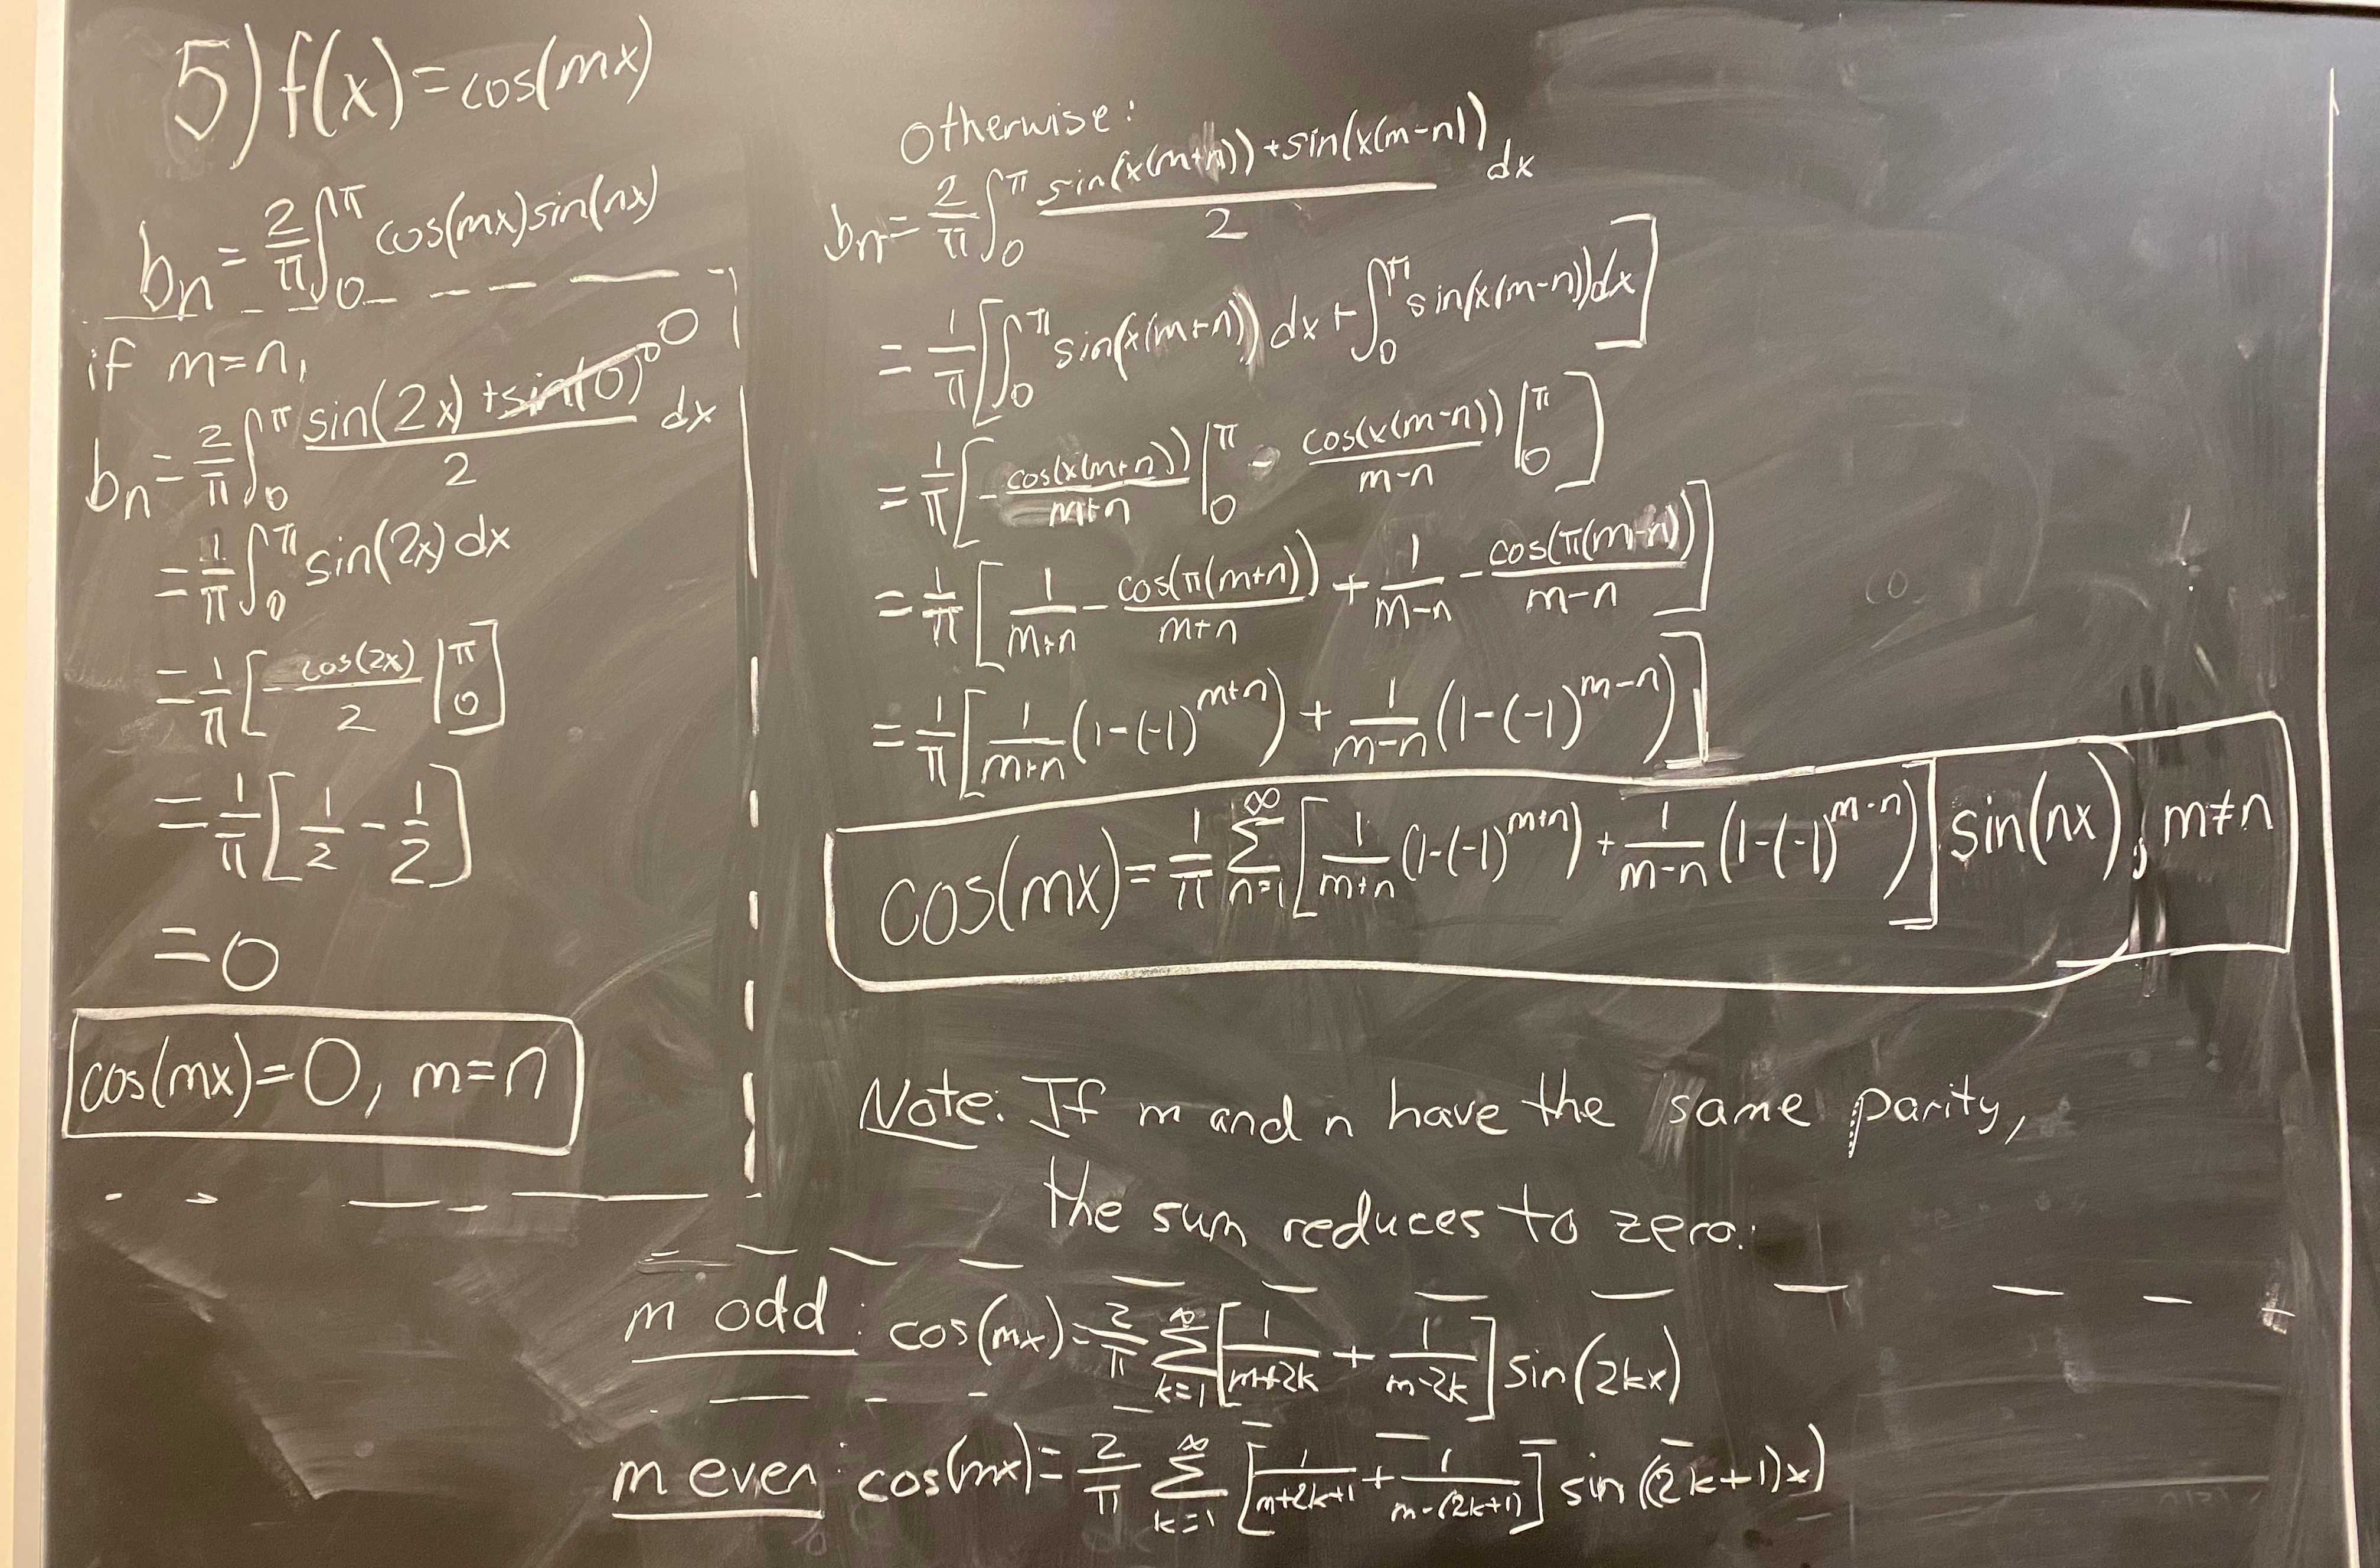
\includegraphics[width = 0.9\textwidth]{Problem 4-5.png}
        \end{figure}
        
        \item \phantom{.} \begin{figure}[H]
            \centering
            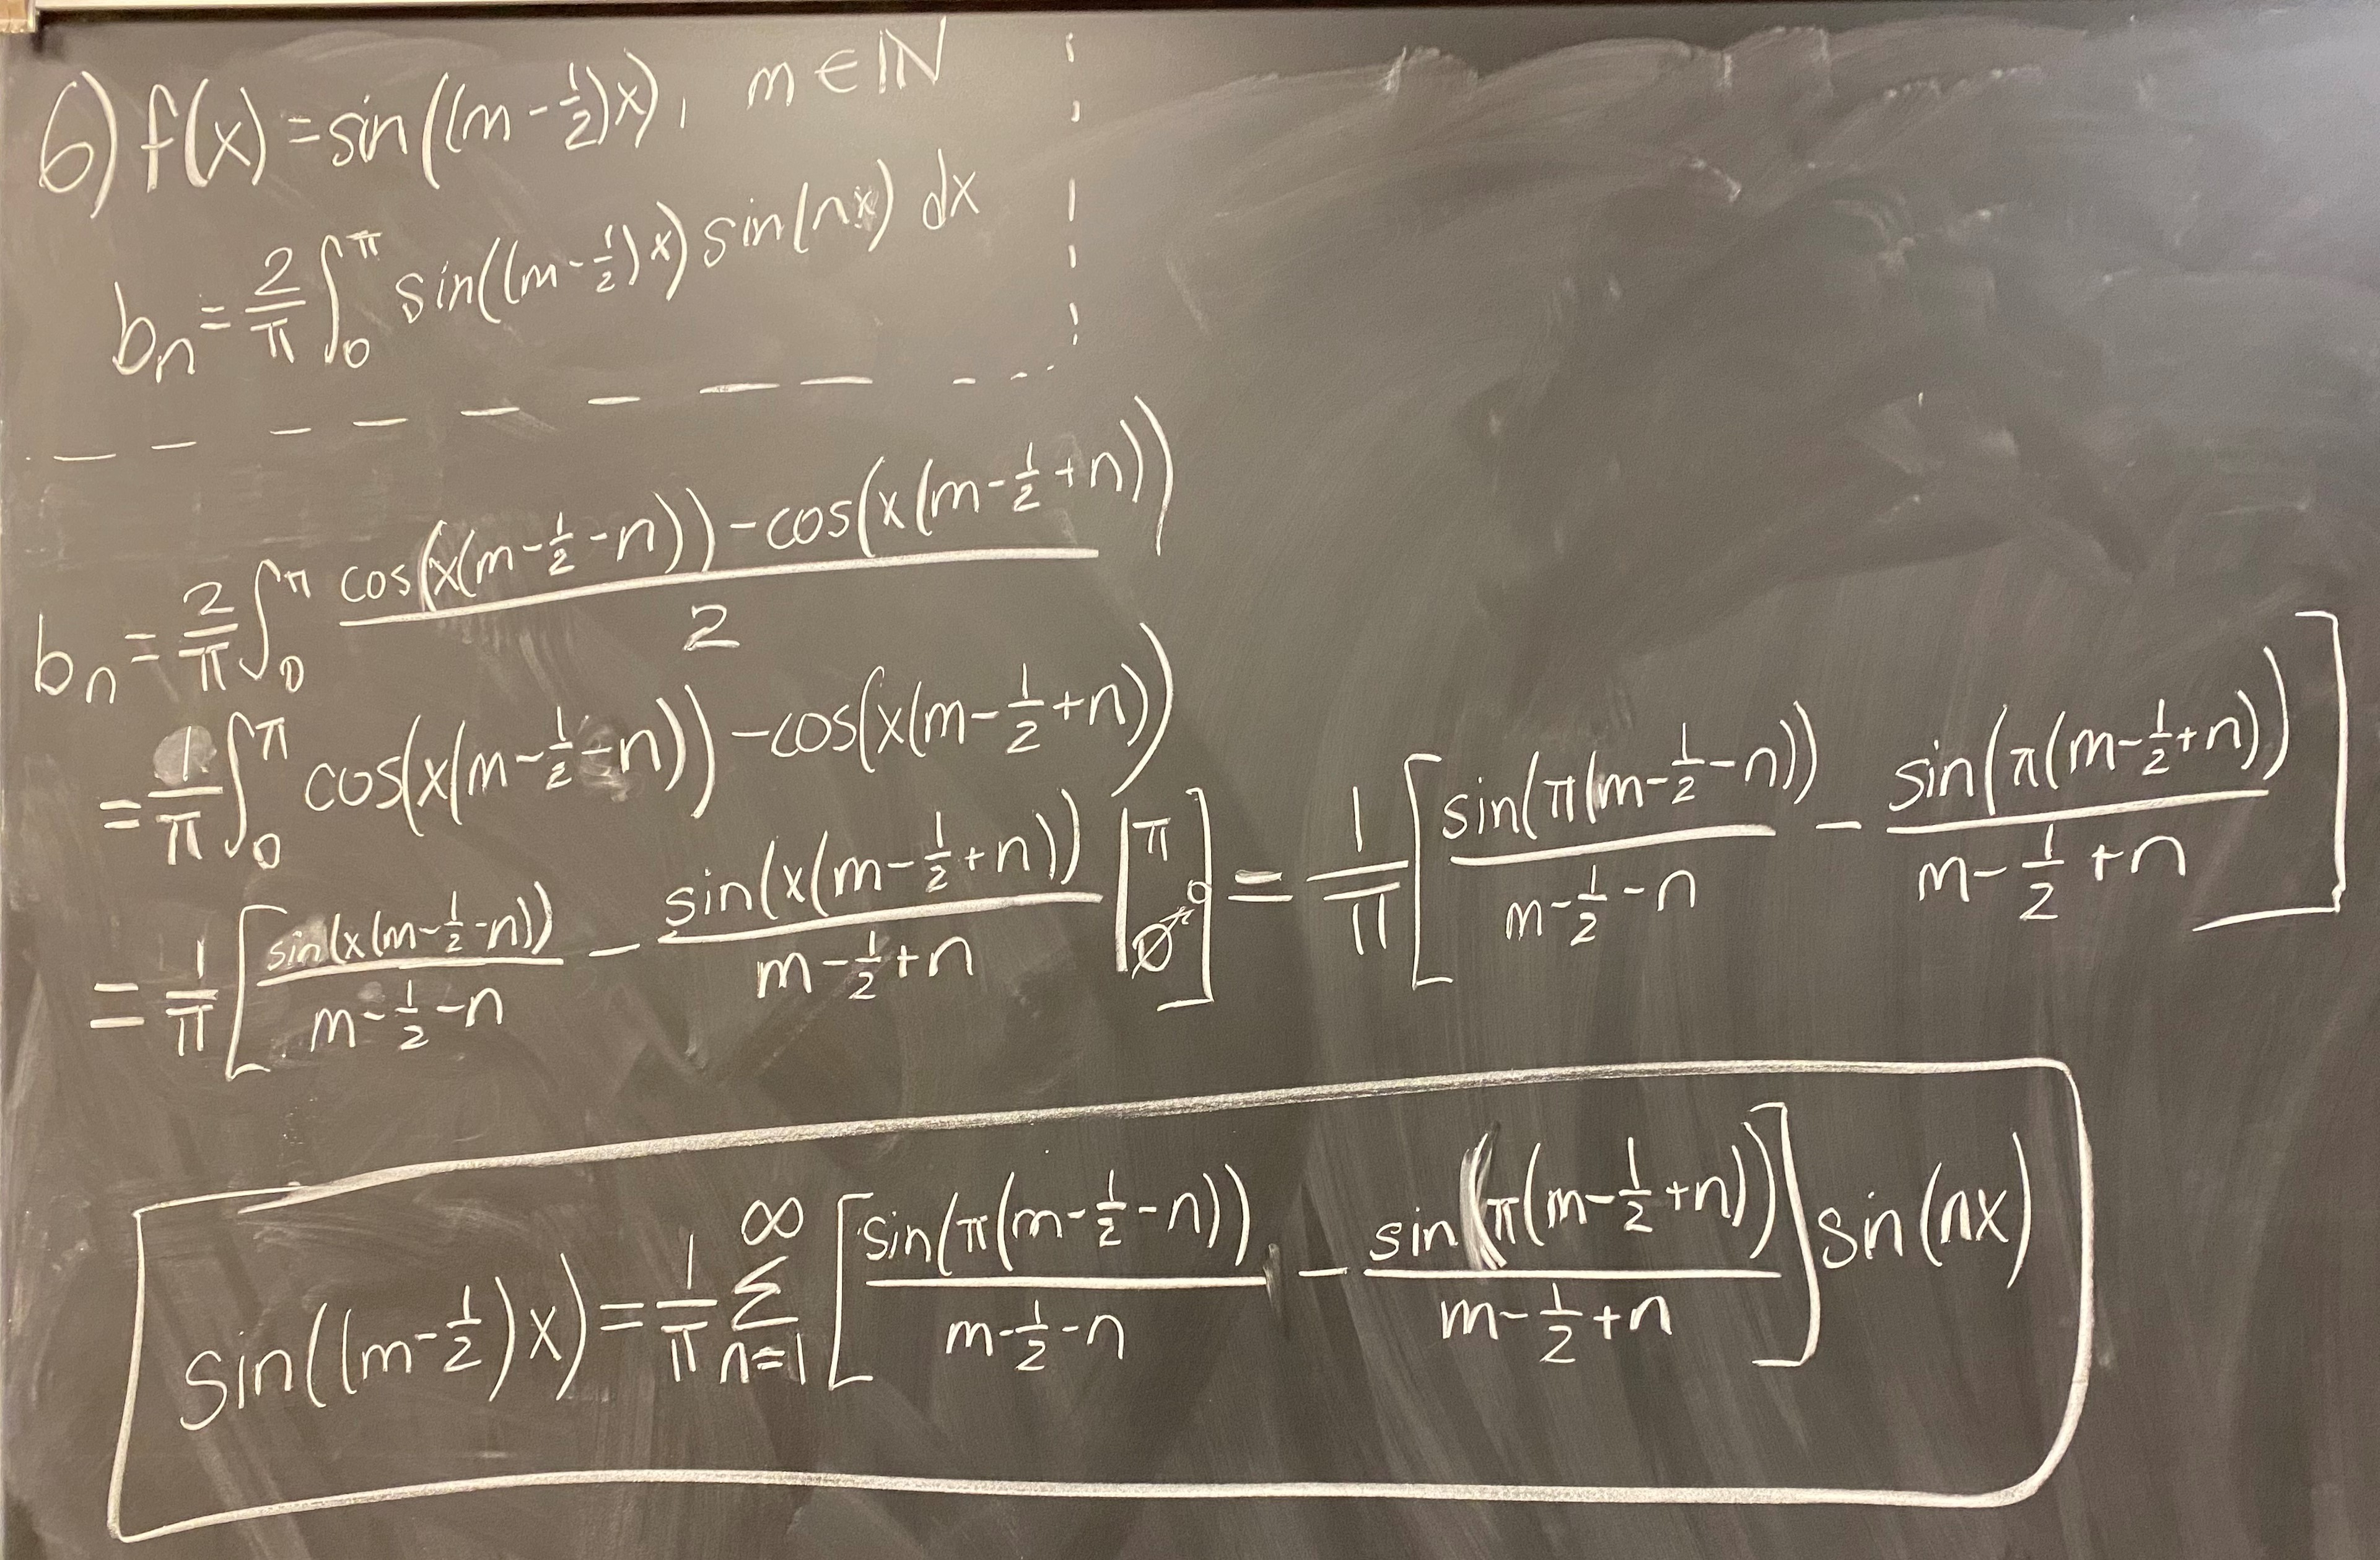
\includegraphics[width = 0.9\textwidth]{Problem 4-6.png}
        \end{figure}
    \end{enumerate}
\end{ans}

\begin{boldenv}
    \underline{Problem 5}. Decompose into cos-Fourier series on interval $[0, \pi]$ and sketch the graph of the sum of such Fourier series: \begin{align}
        & 1\\
        & x\\
        & x(\pi - x)\\
        & \sin(mx) \text{ with } m \in \N\\
        & \cos(mx) \text{ with } m \in \N\\
        & \sin((m - \frac{1}{2})x) \text{ with } m \in \N
    \end{align}
\end{boldenv}
\begin{ans}
Similar to Problem 4, this question wants us to use a specific Fourier series, in this case the cosine Fourier series. The formula for this is
\begin{figure}[H]
\centering
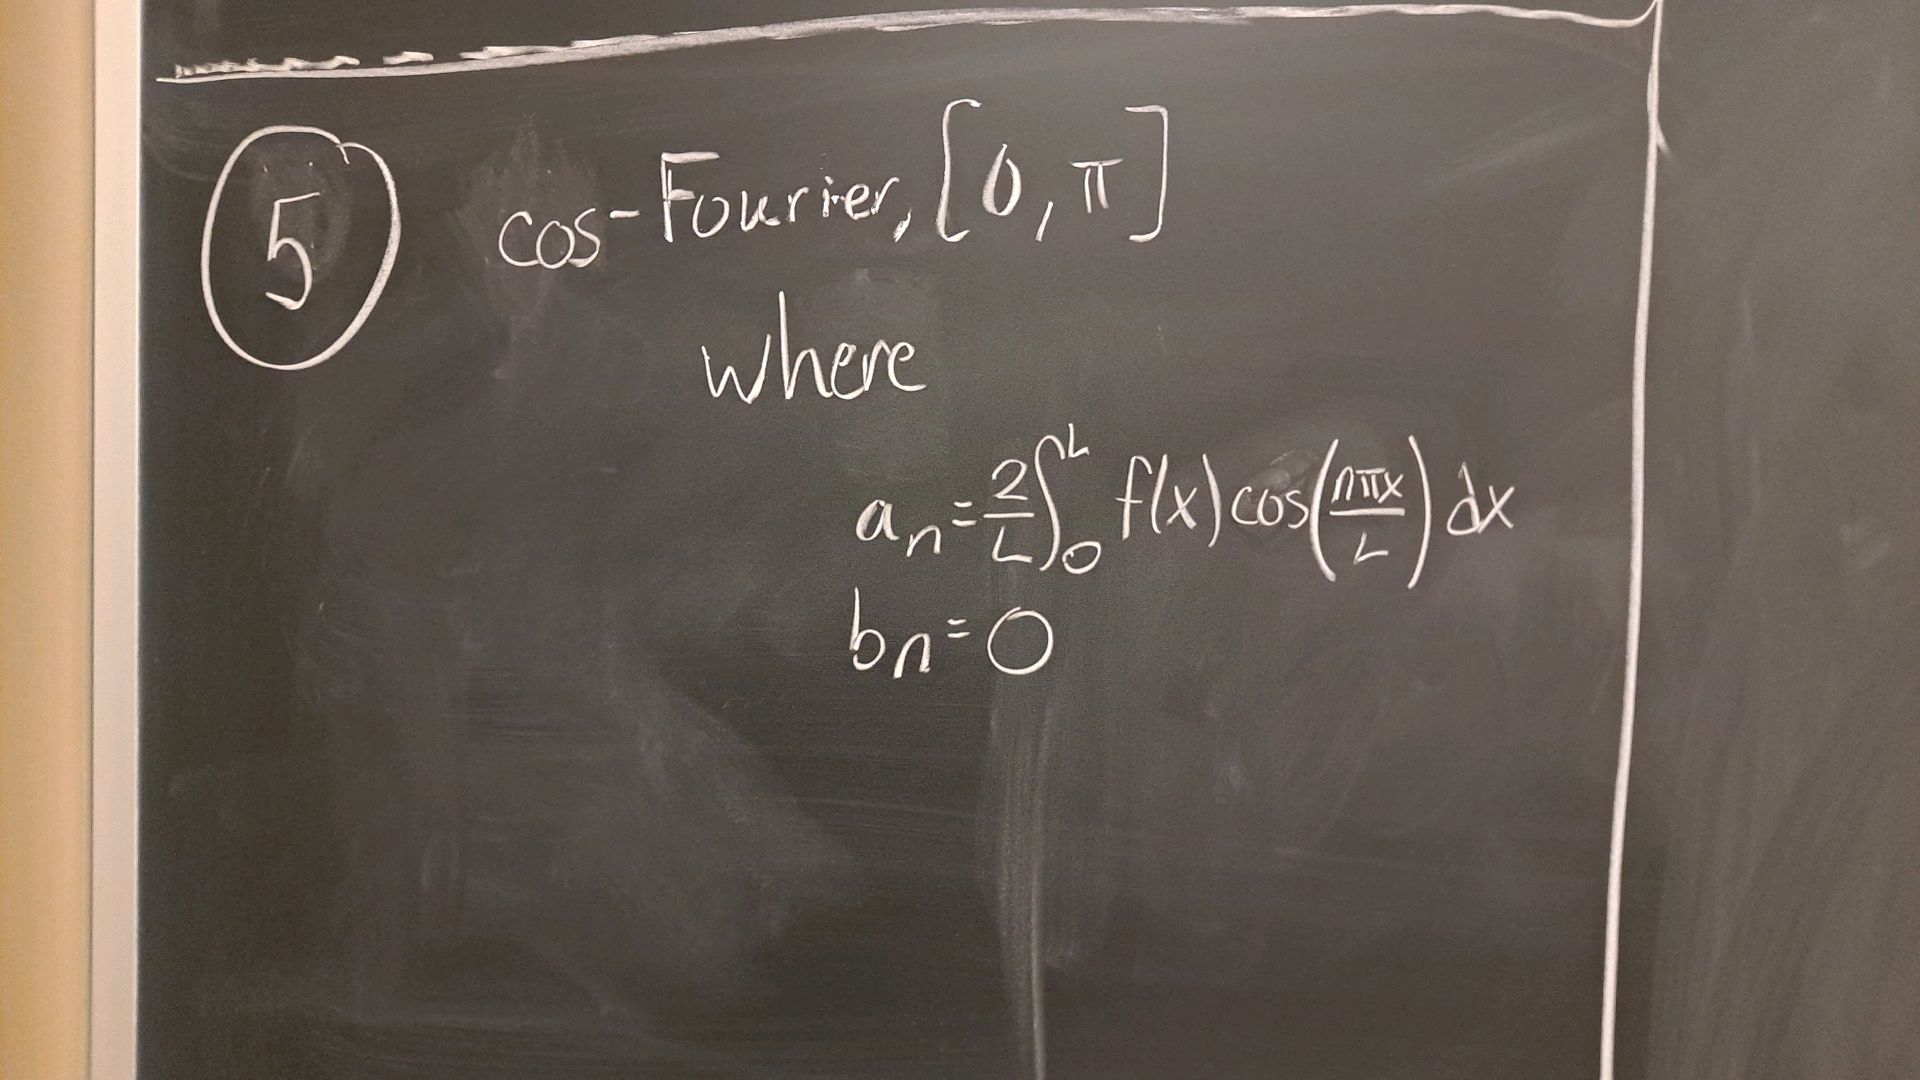
\includegraphics[width = 0.55\textwidth]{Problem 5 format.jpeg}
\end{figure}
    \begin{enumerate}
        \item \phantom{.} \begin{figure}[H]
\centering
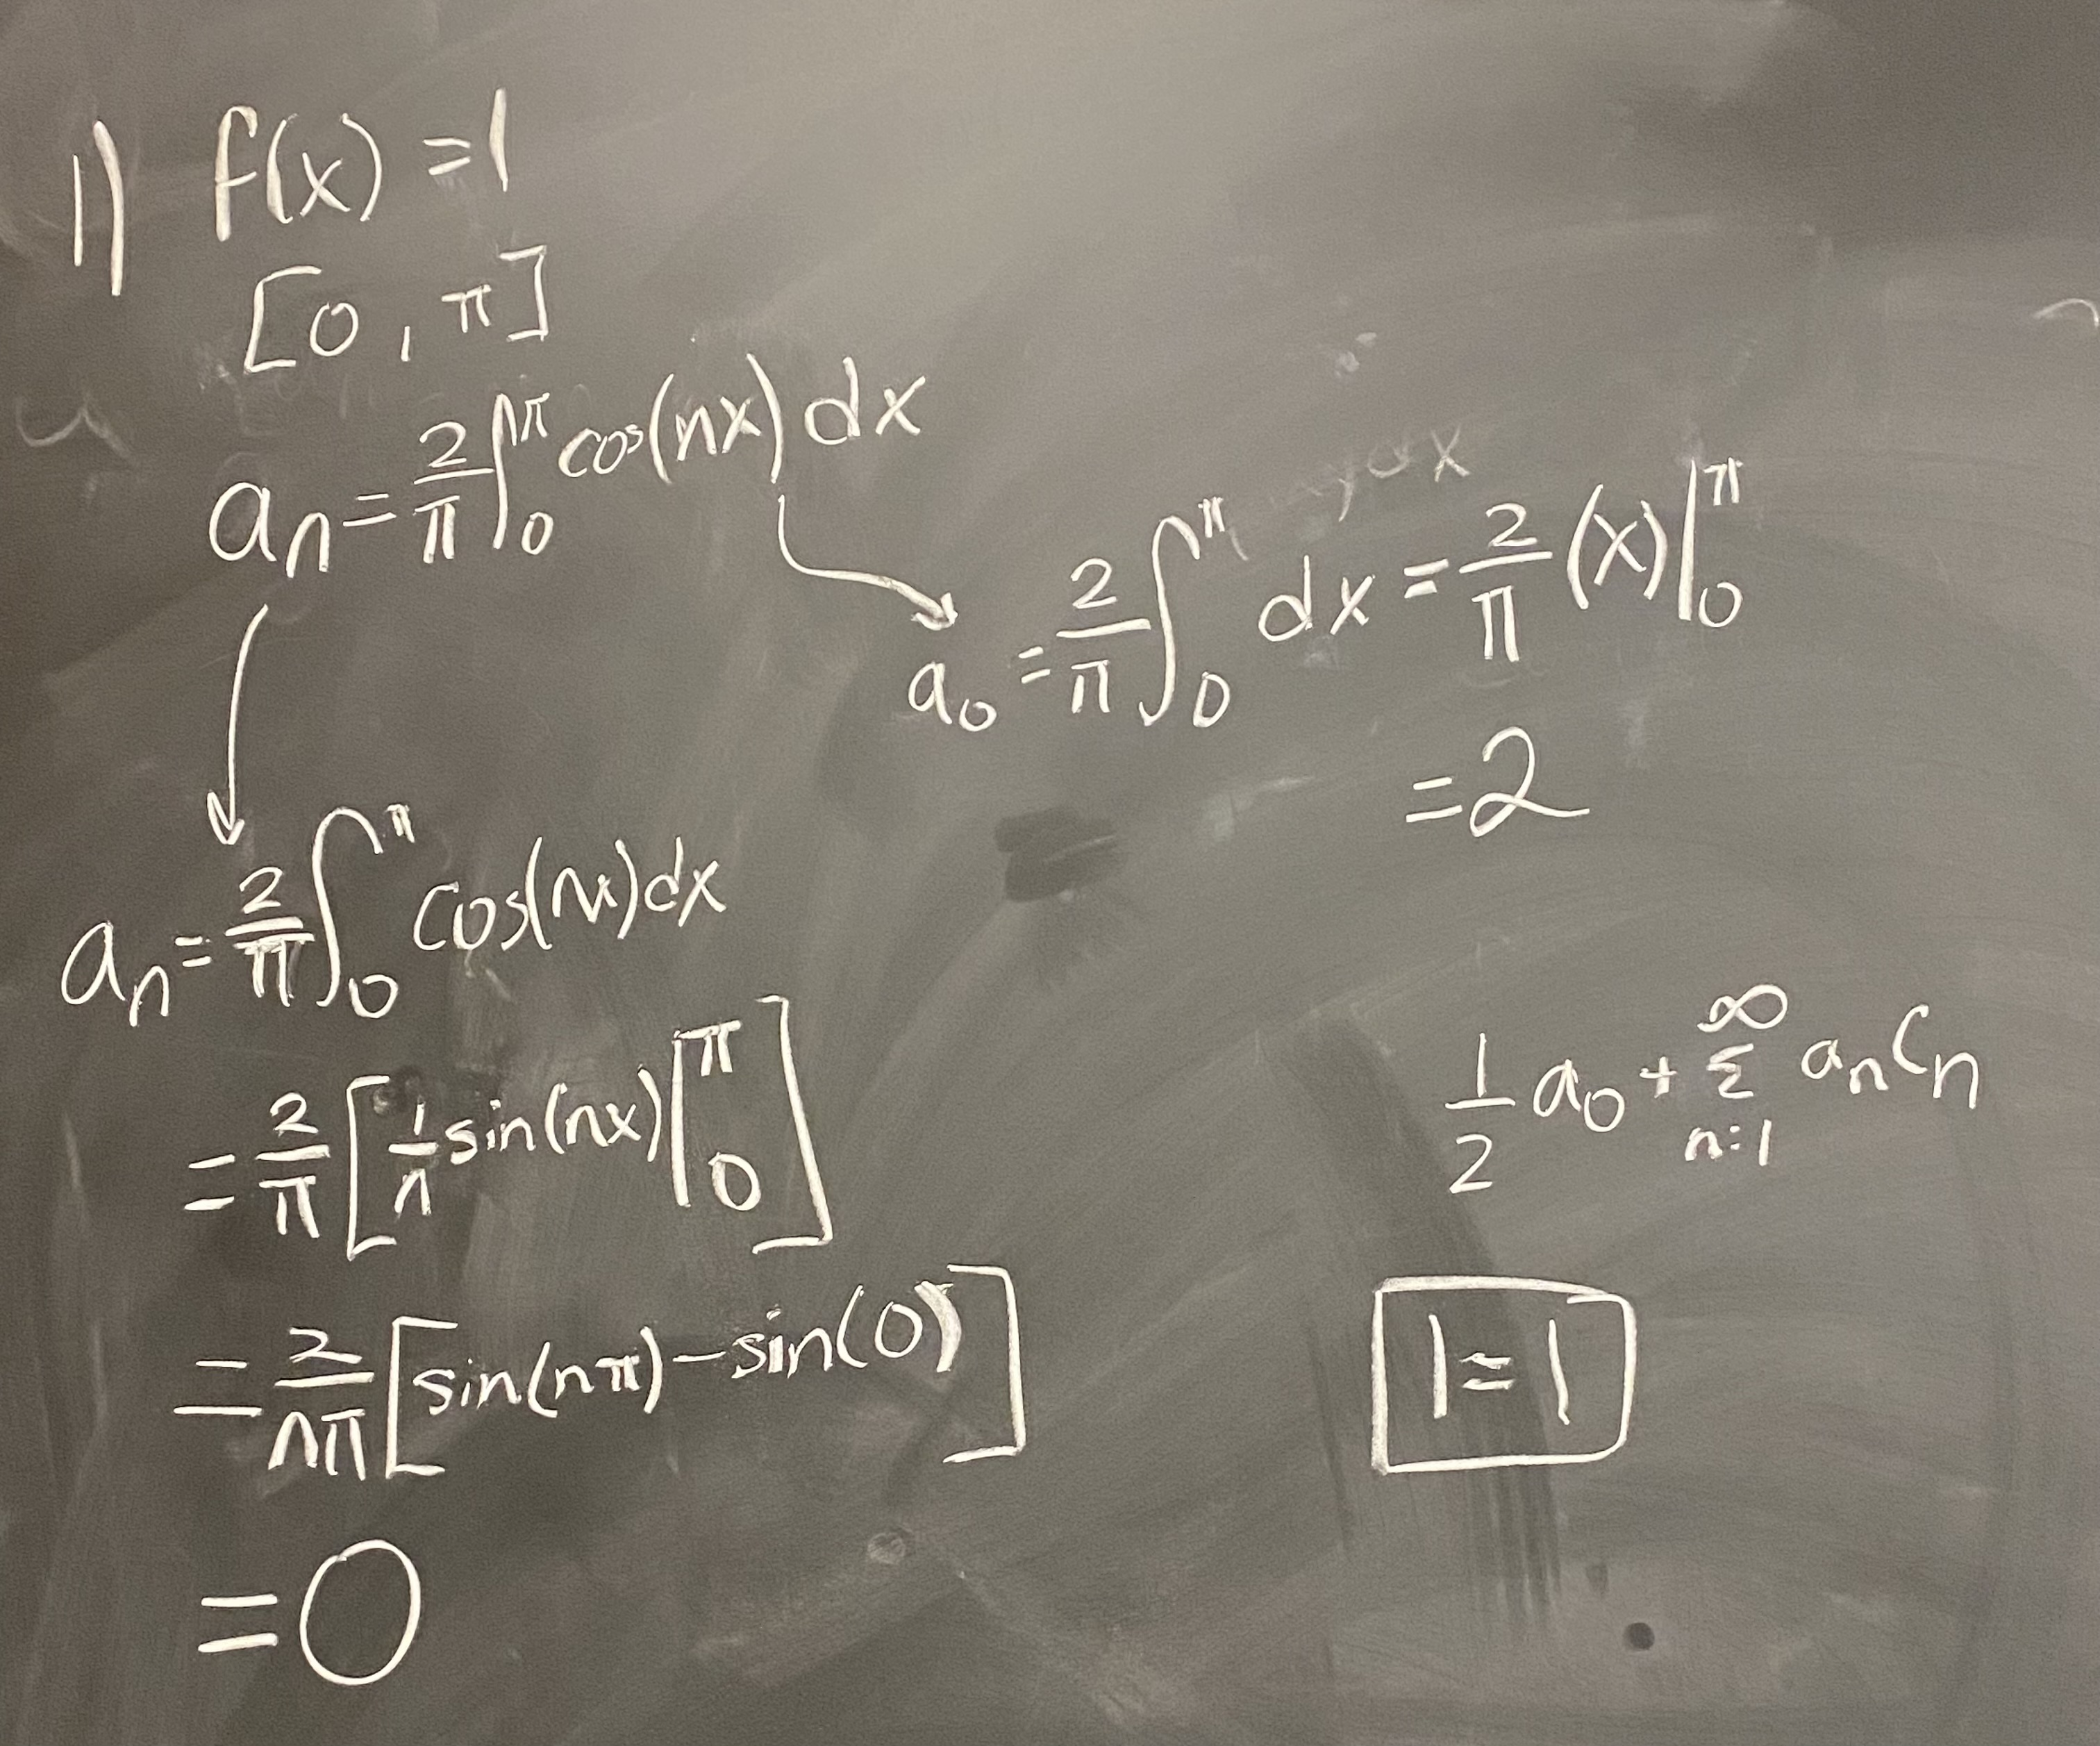
\includegraphics[width = 0.75\textwidth]{Problem 5-1.jpg}
\end{figure}
\begin{figure}
    \centering
    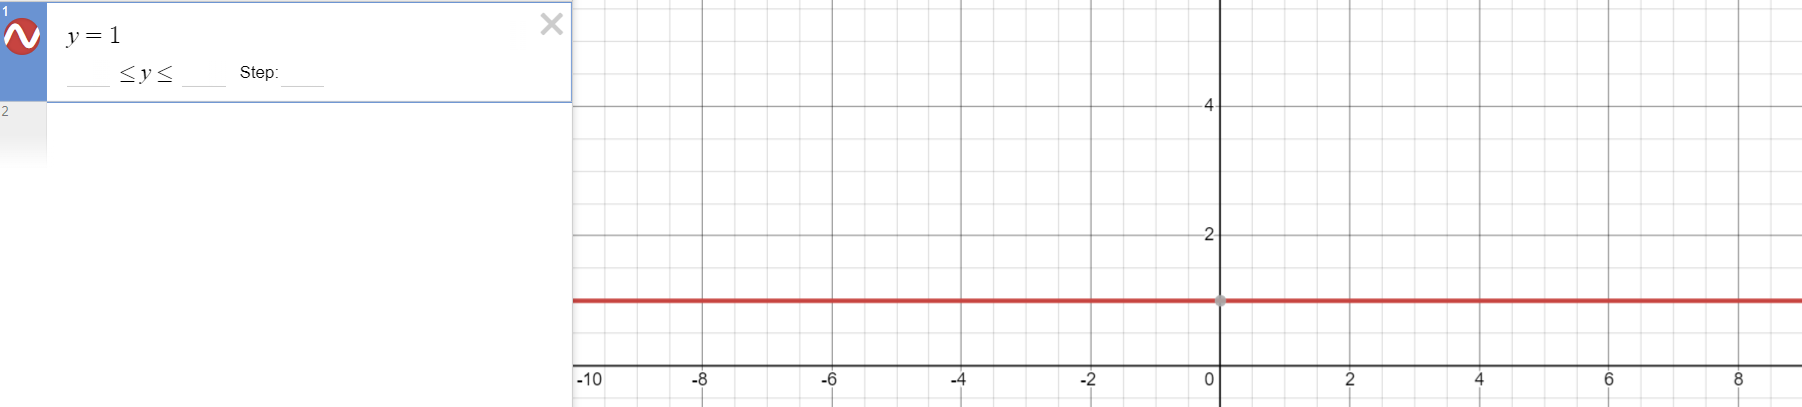
\includegraphics[width = 0.75\textwidth]{Problem 5.1.png}
\end{figure}

        \item \phantom{.} \begin{figure}[H]
            \centering
            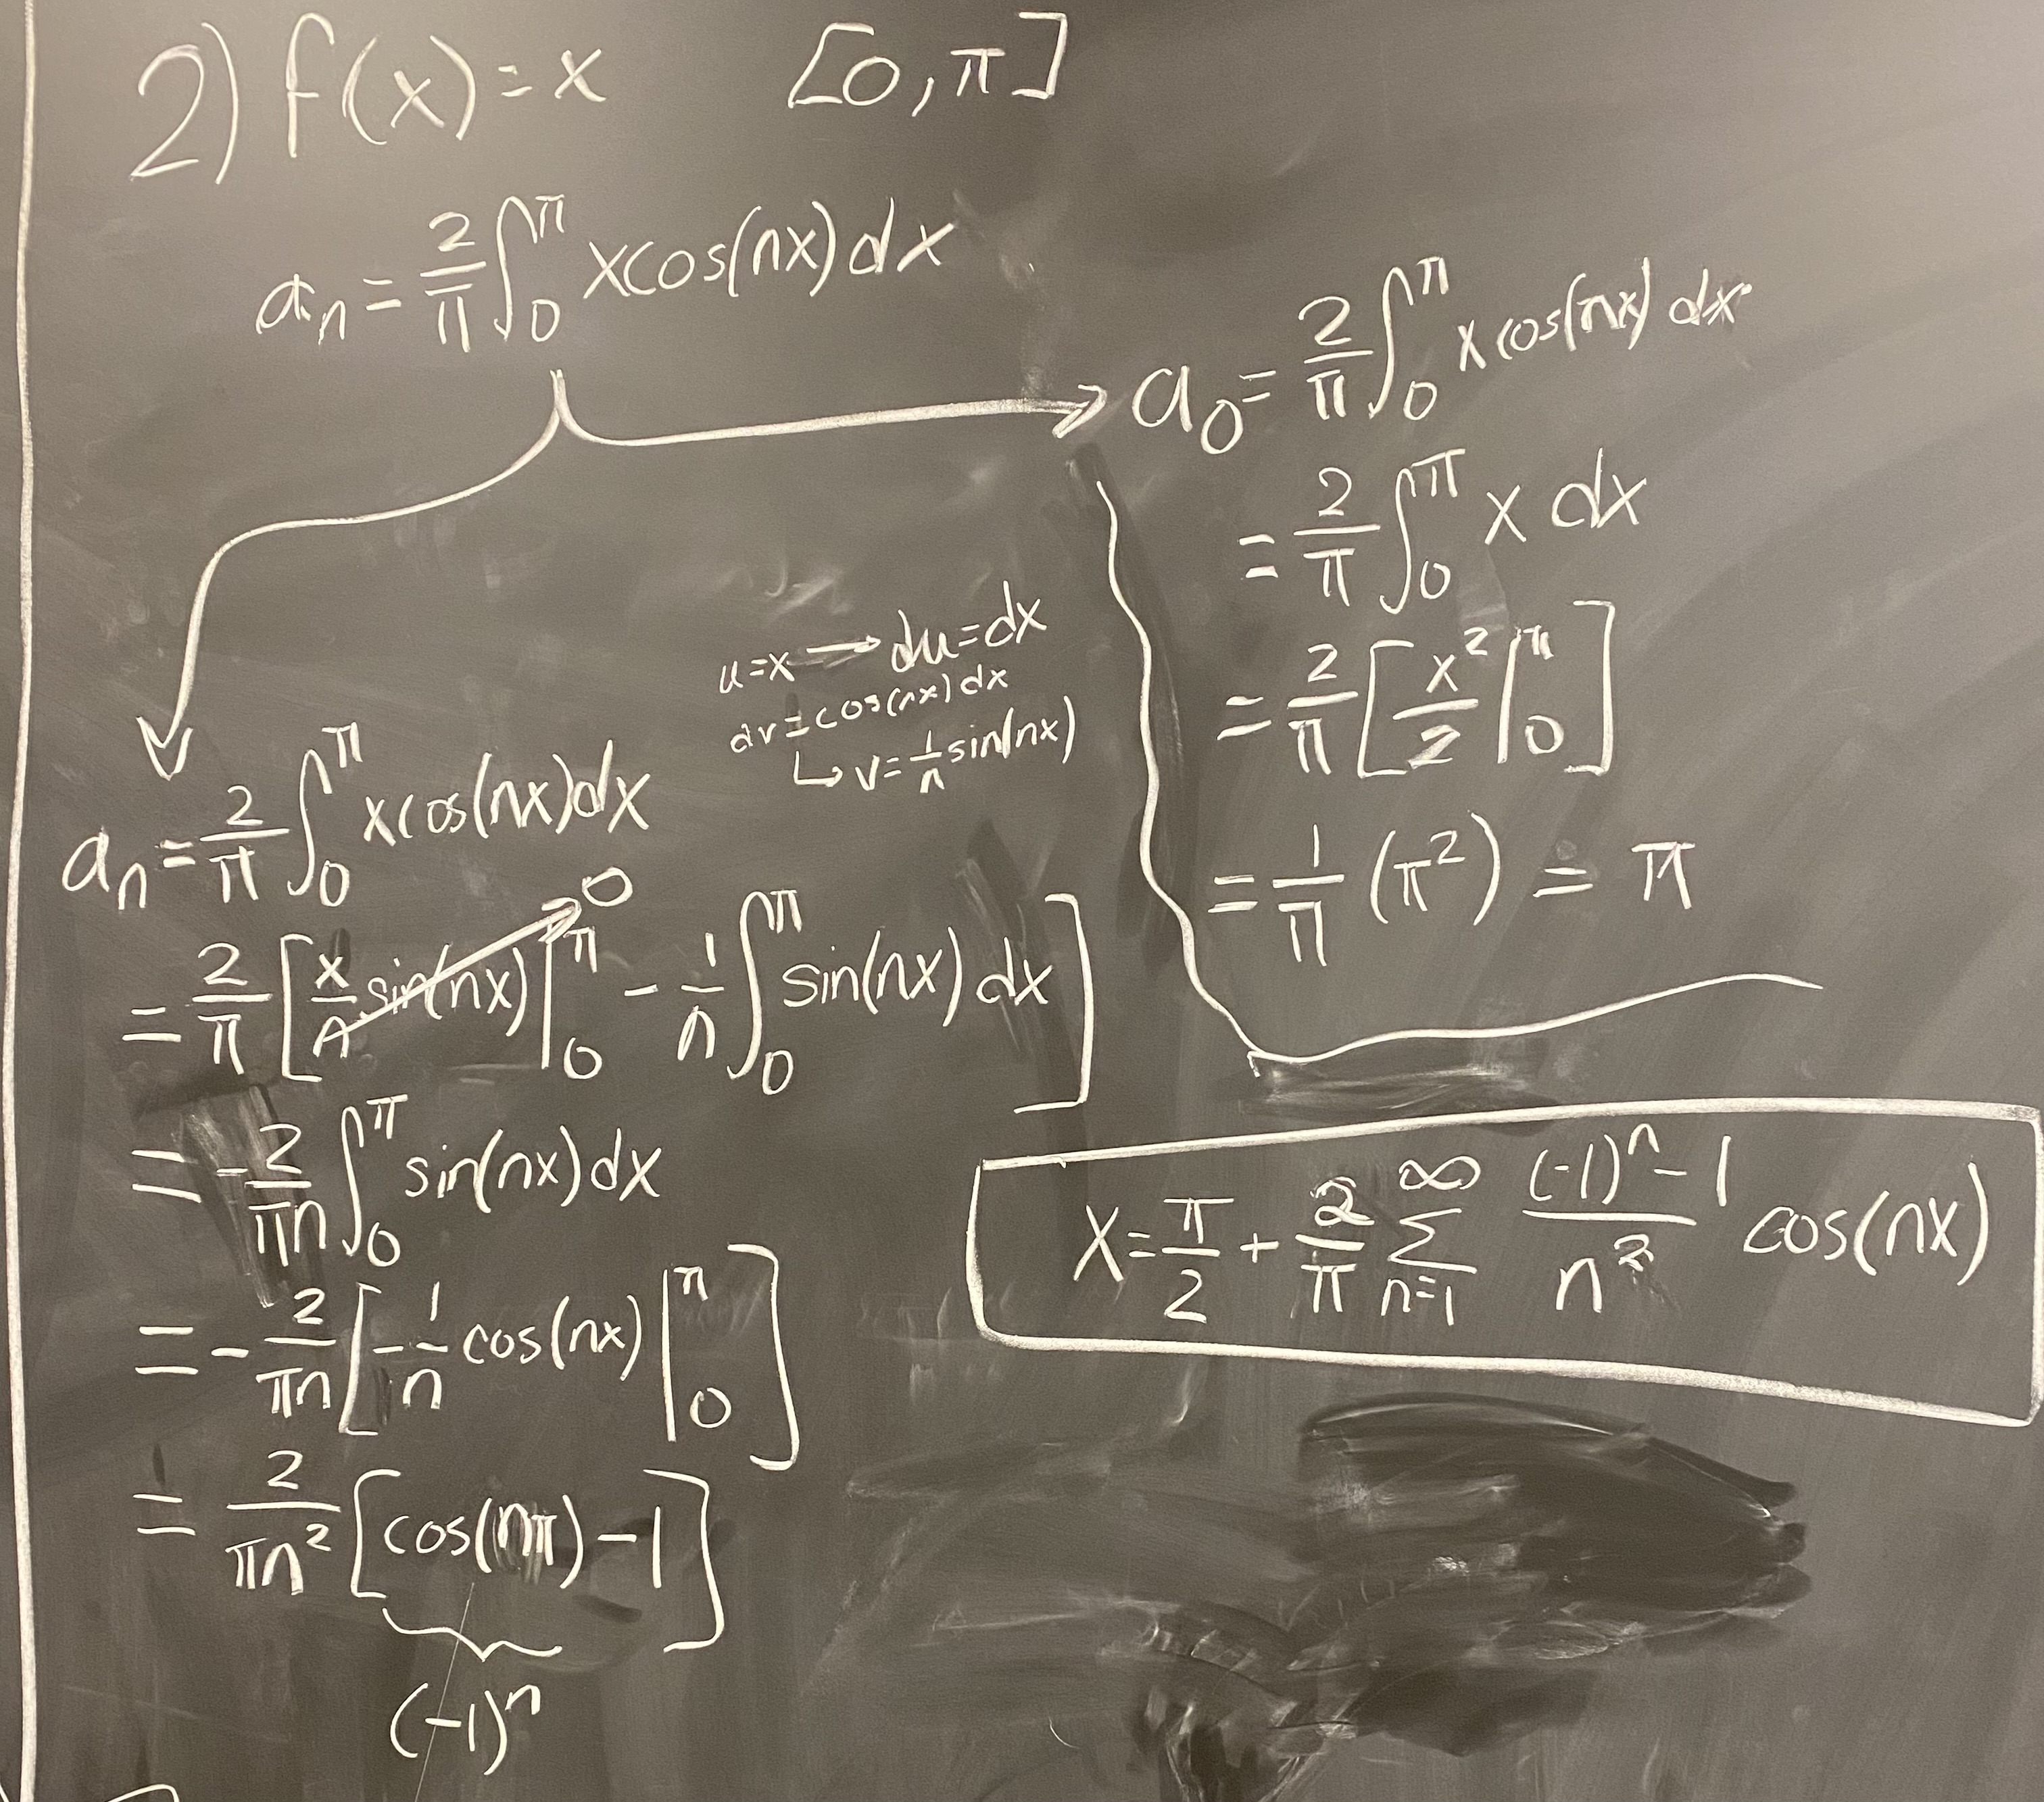
\includegraphics[width = \textwidth]{Problem 5-2.jpg}
            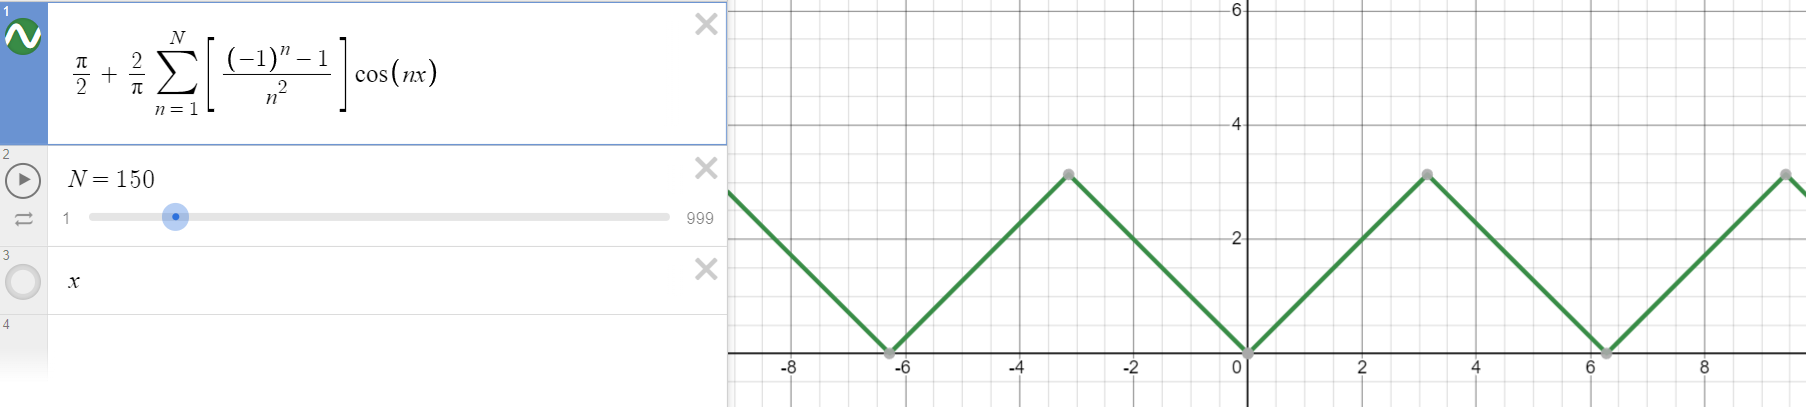
\includegraphics[width = \textwidth]{Problem 5.2.png}
        \end{figure}

        \item \phantom{.} \begin{figure}[H]
            \centering
            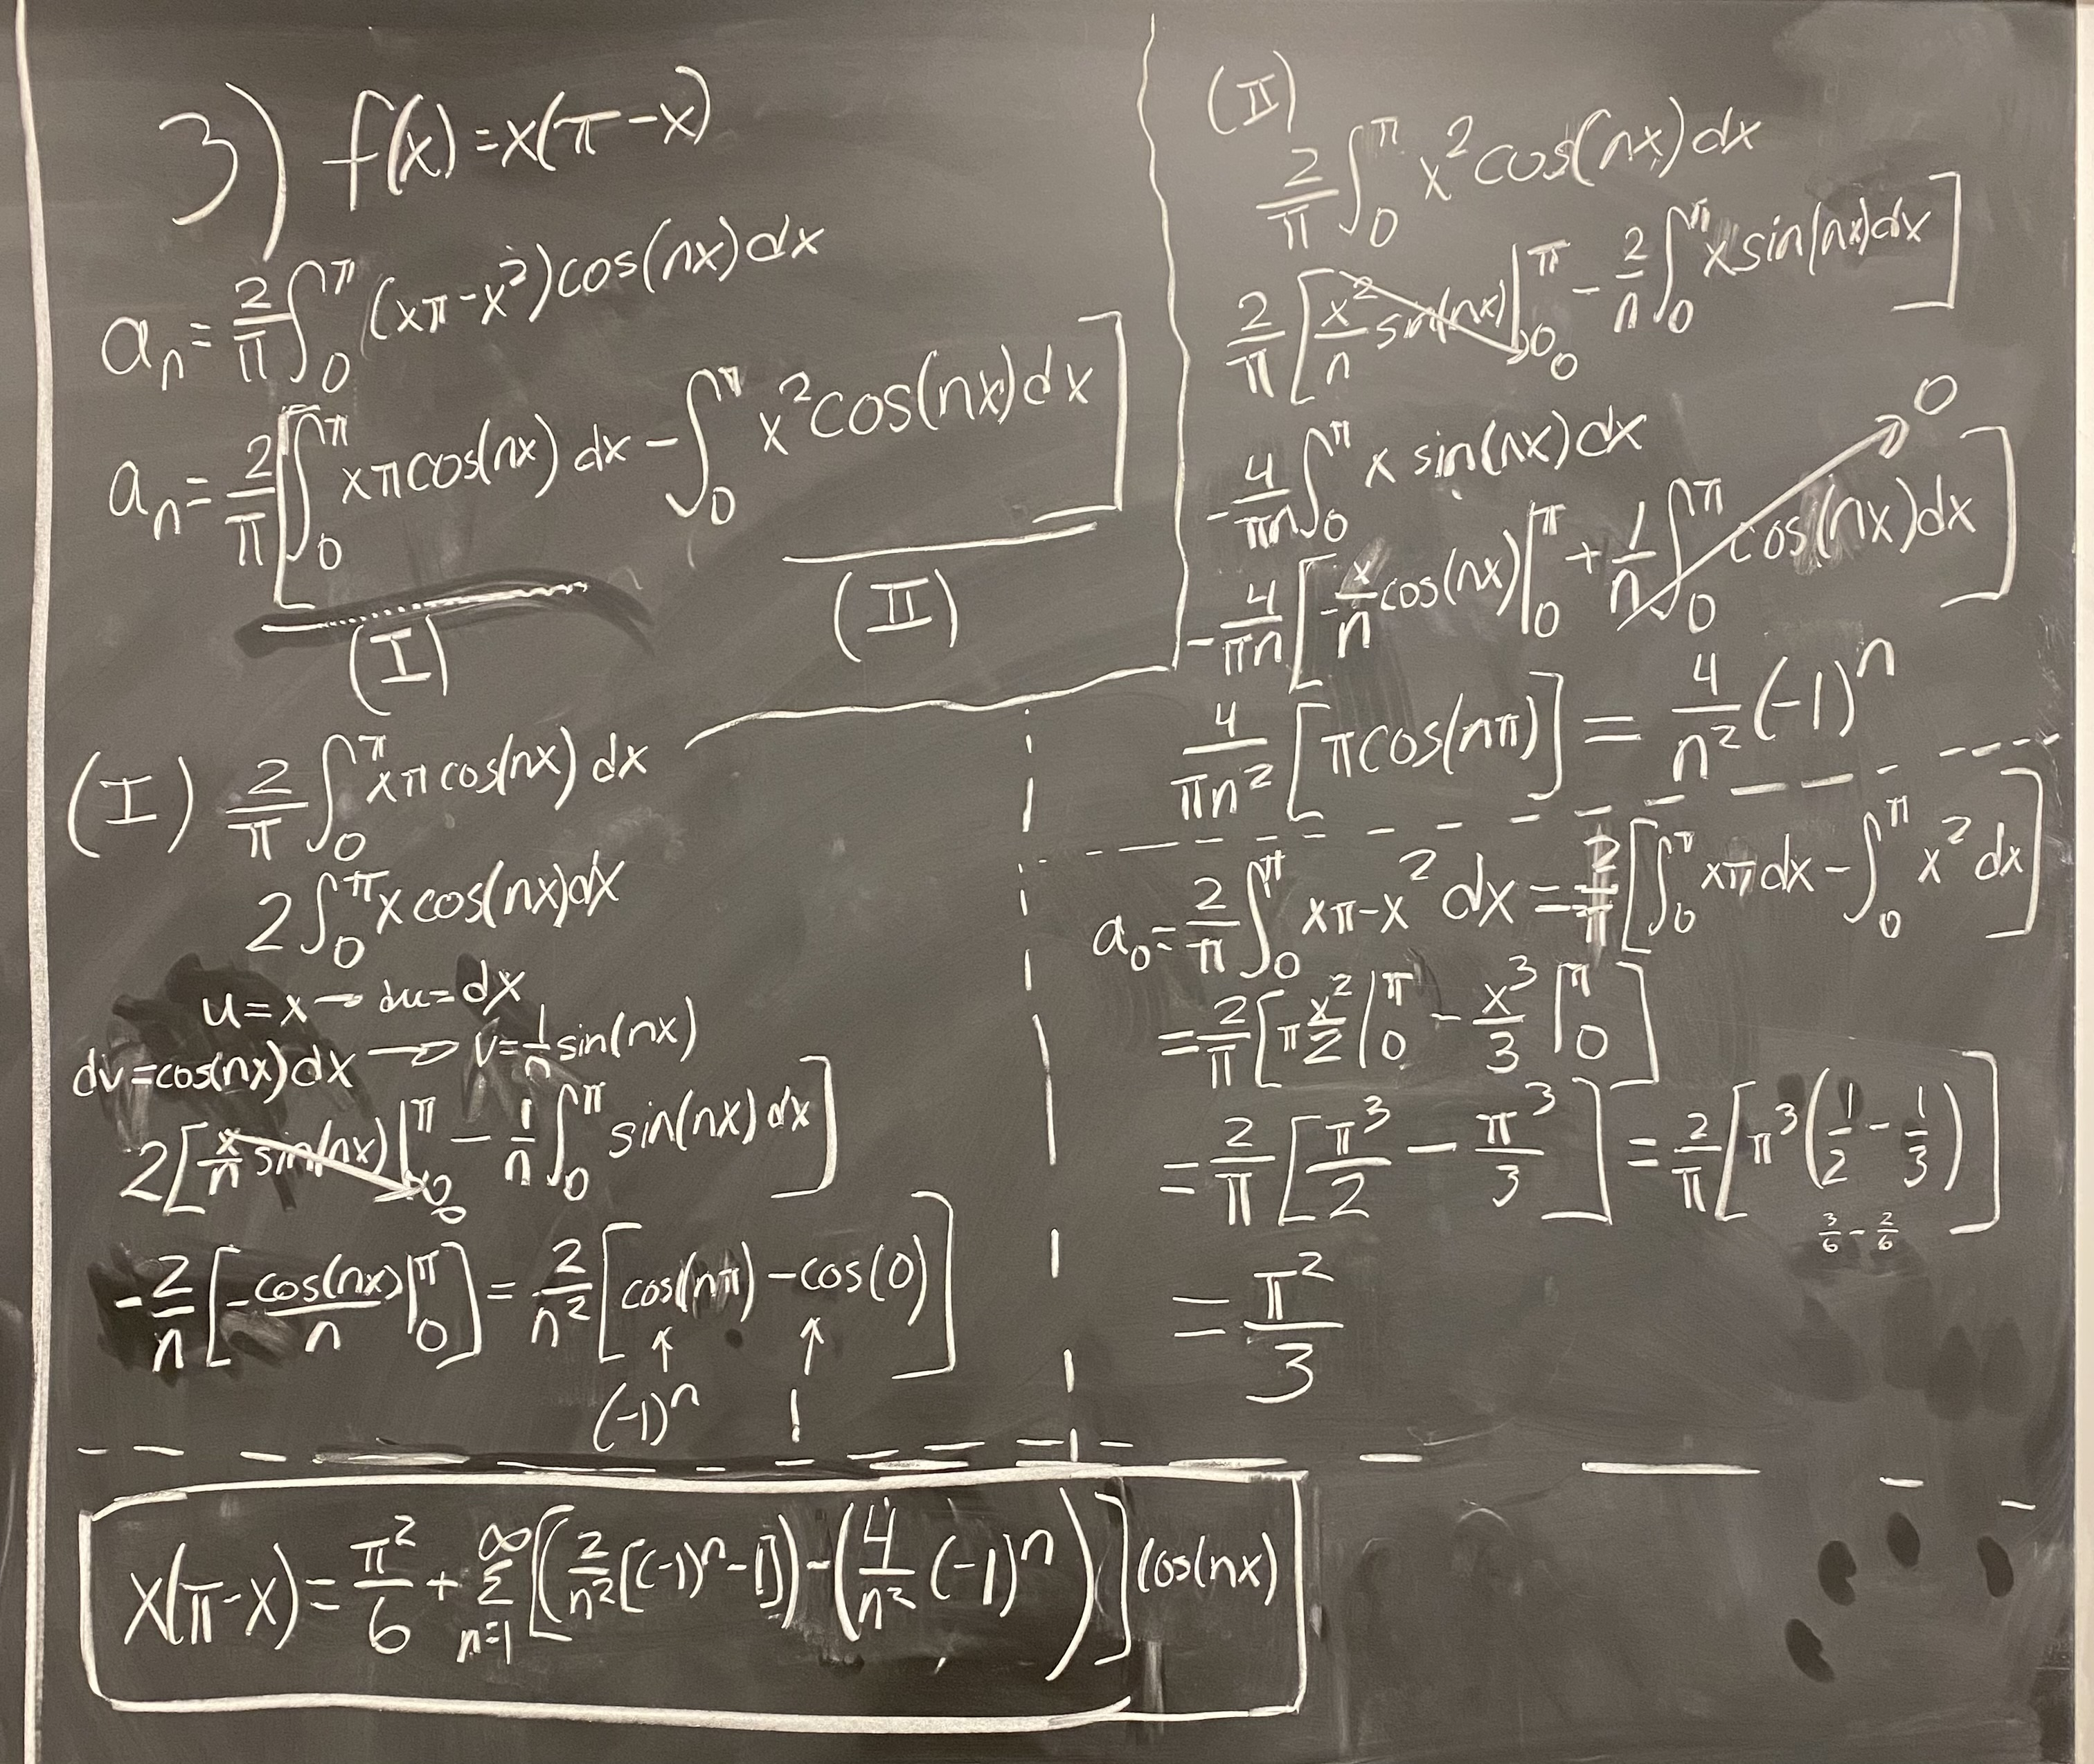
\includegraphics[width = \textwidth]{Problem 5-3.jpg}
            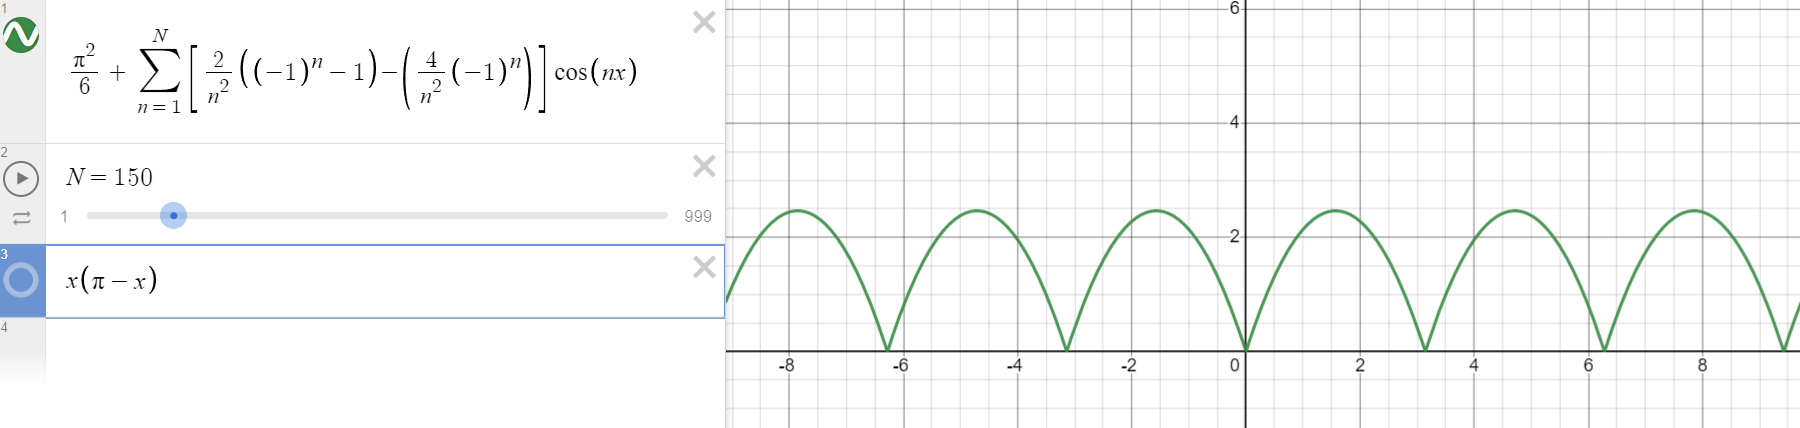
\includegraphics[width = \textwidth]{Problem 5.3.png}
        \end{figure}
\newpage
        \item \phantom{.} \begin{figure}[H]
            \centering
            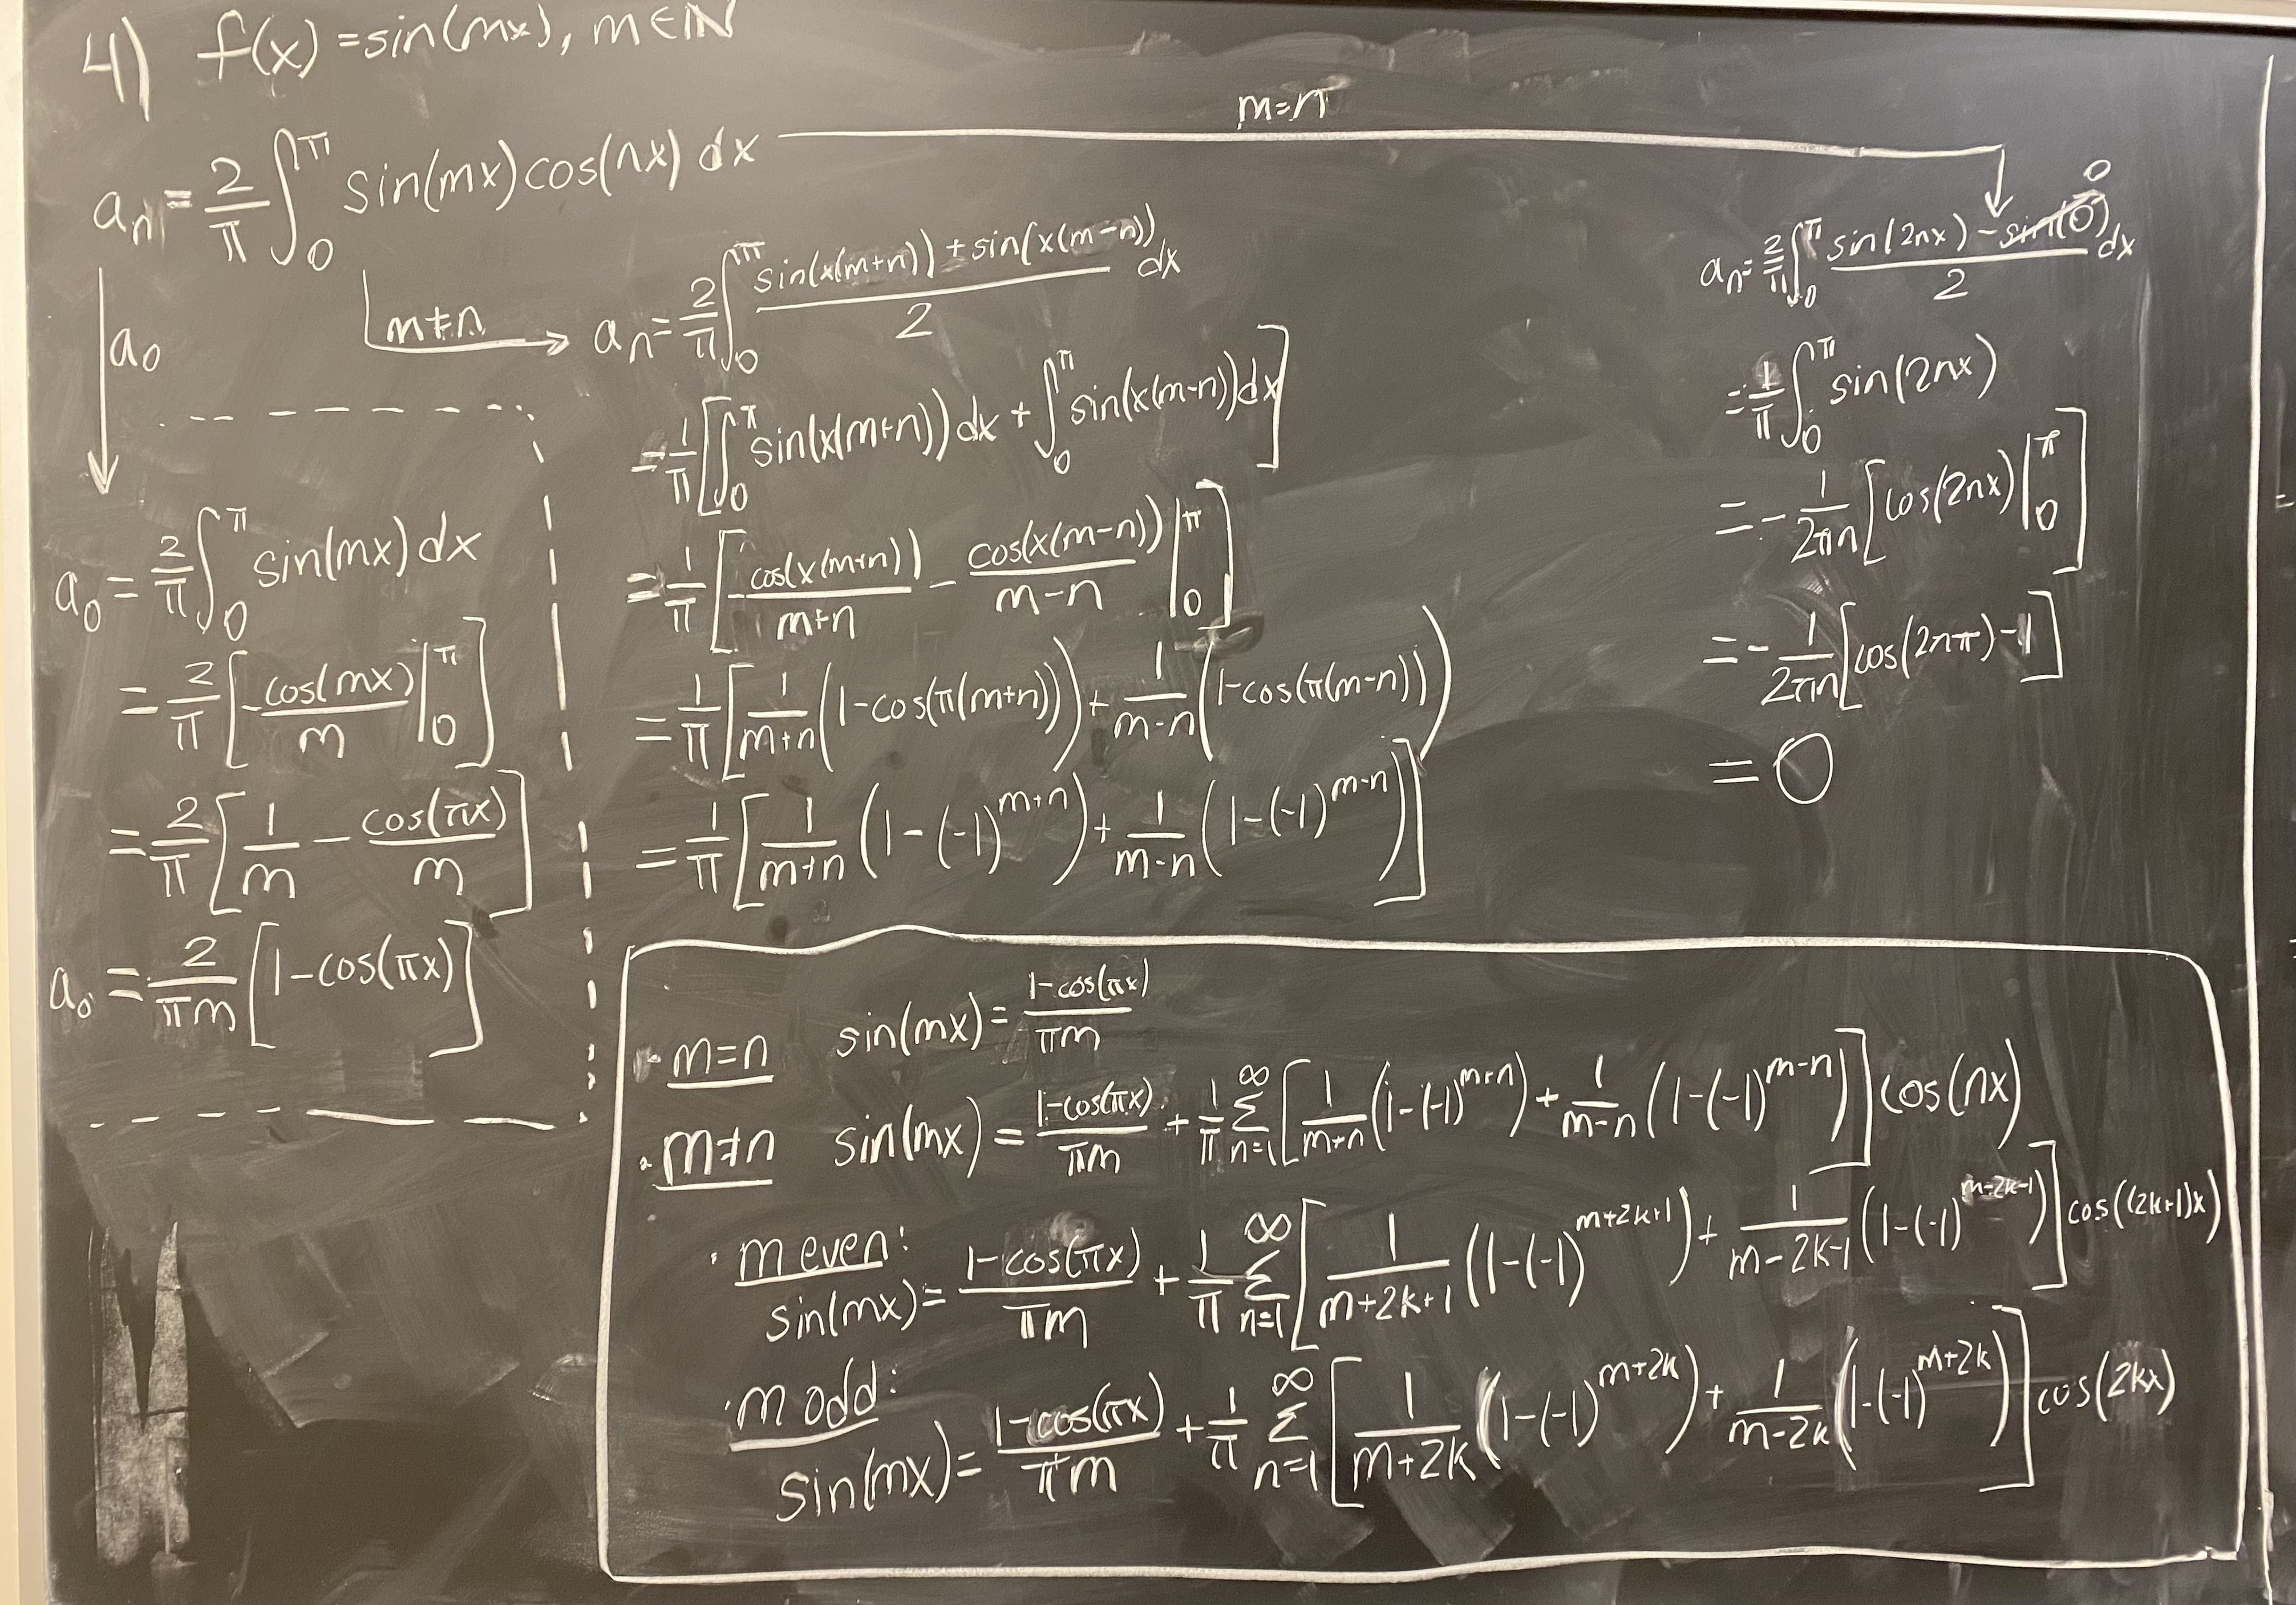
\includegraphics[width = 0.9\textwidth]{Problem 5-4.jpg}
        \end{figure}

        \item \phantom{.} \begin{figure}[H]
            \centering
            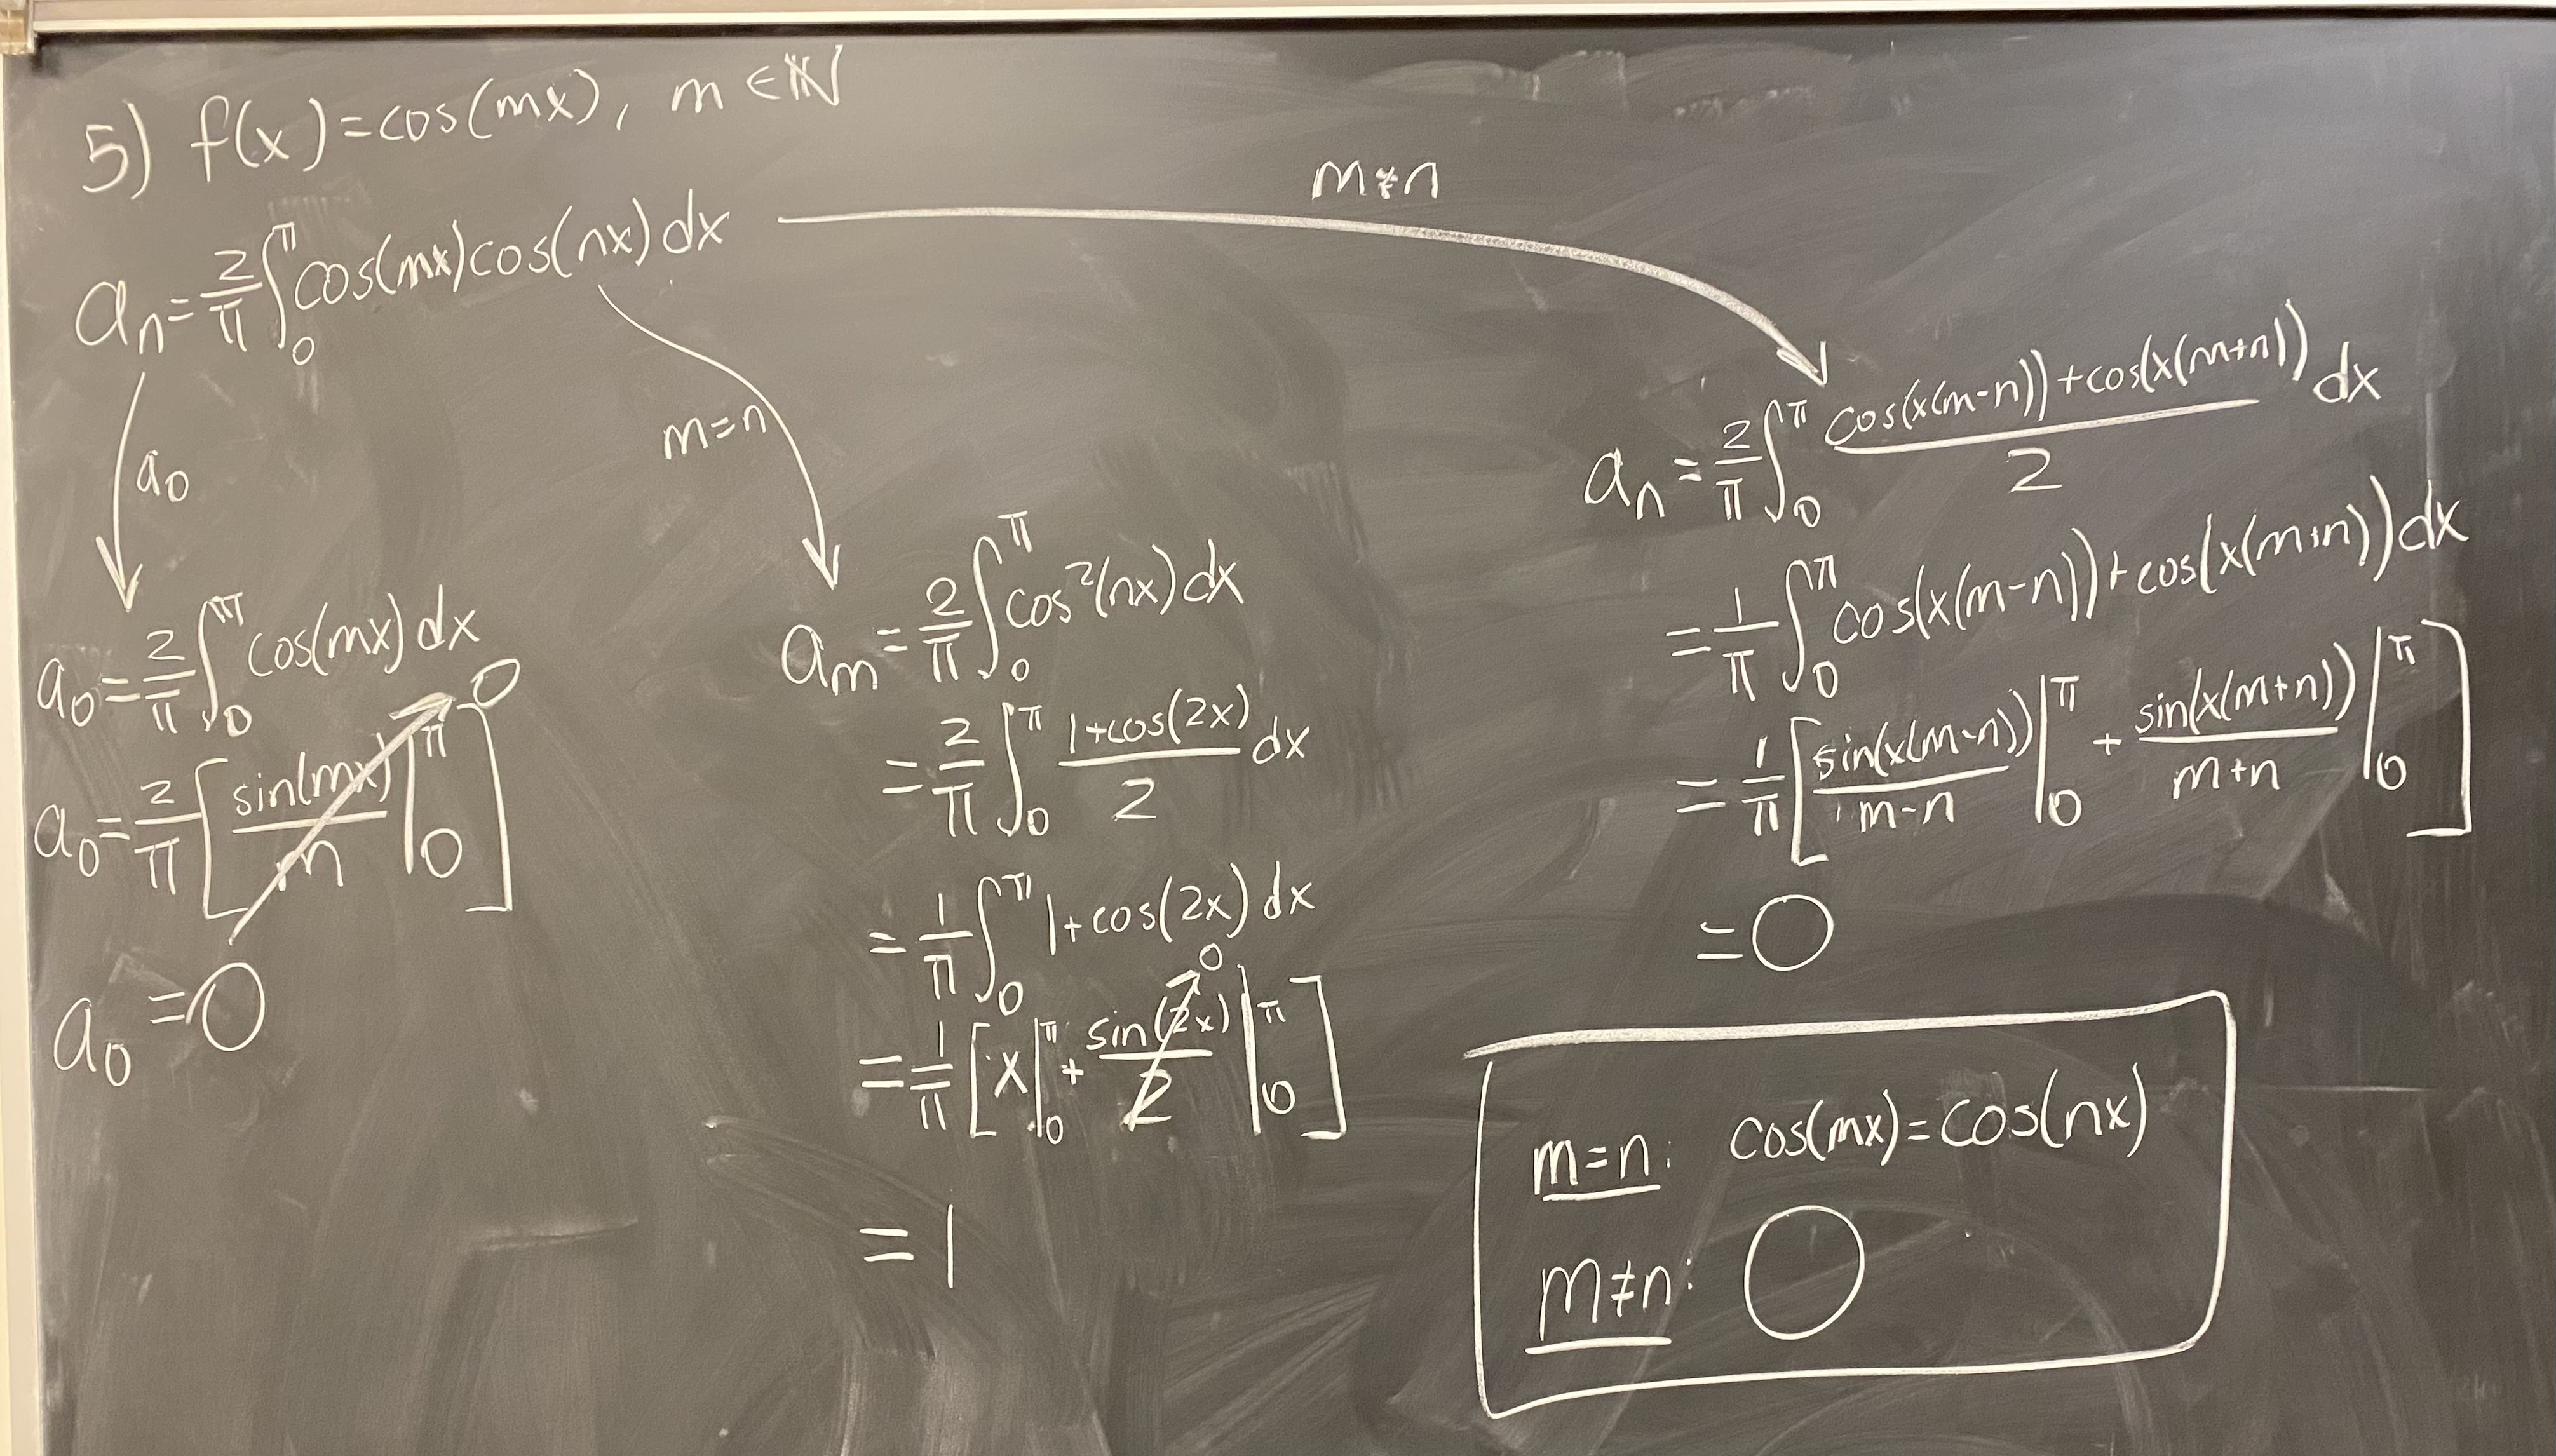
\includegraphics[width = 0.9\textwidth]{Problem 5-5.jpg}
        \end{figure}
\newpage
        \item \phantom{.} \begin{figure}[H]
            \centering
            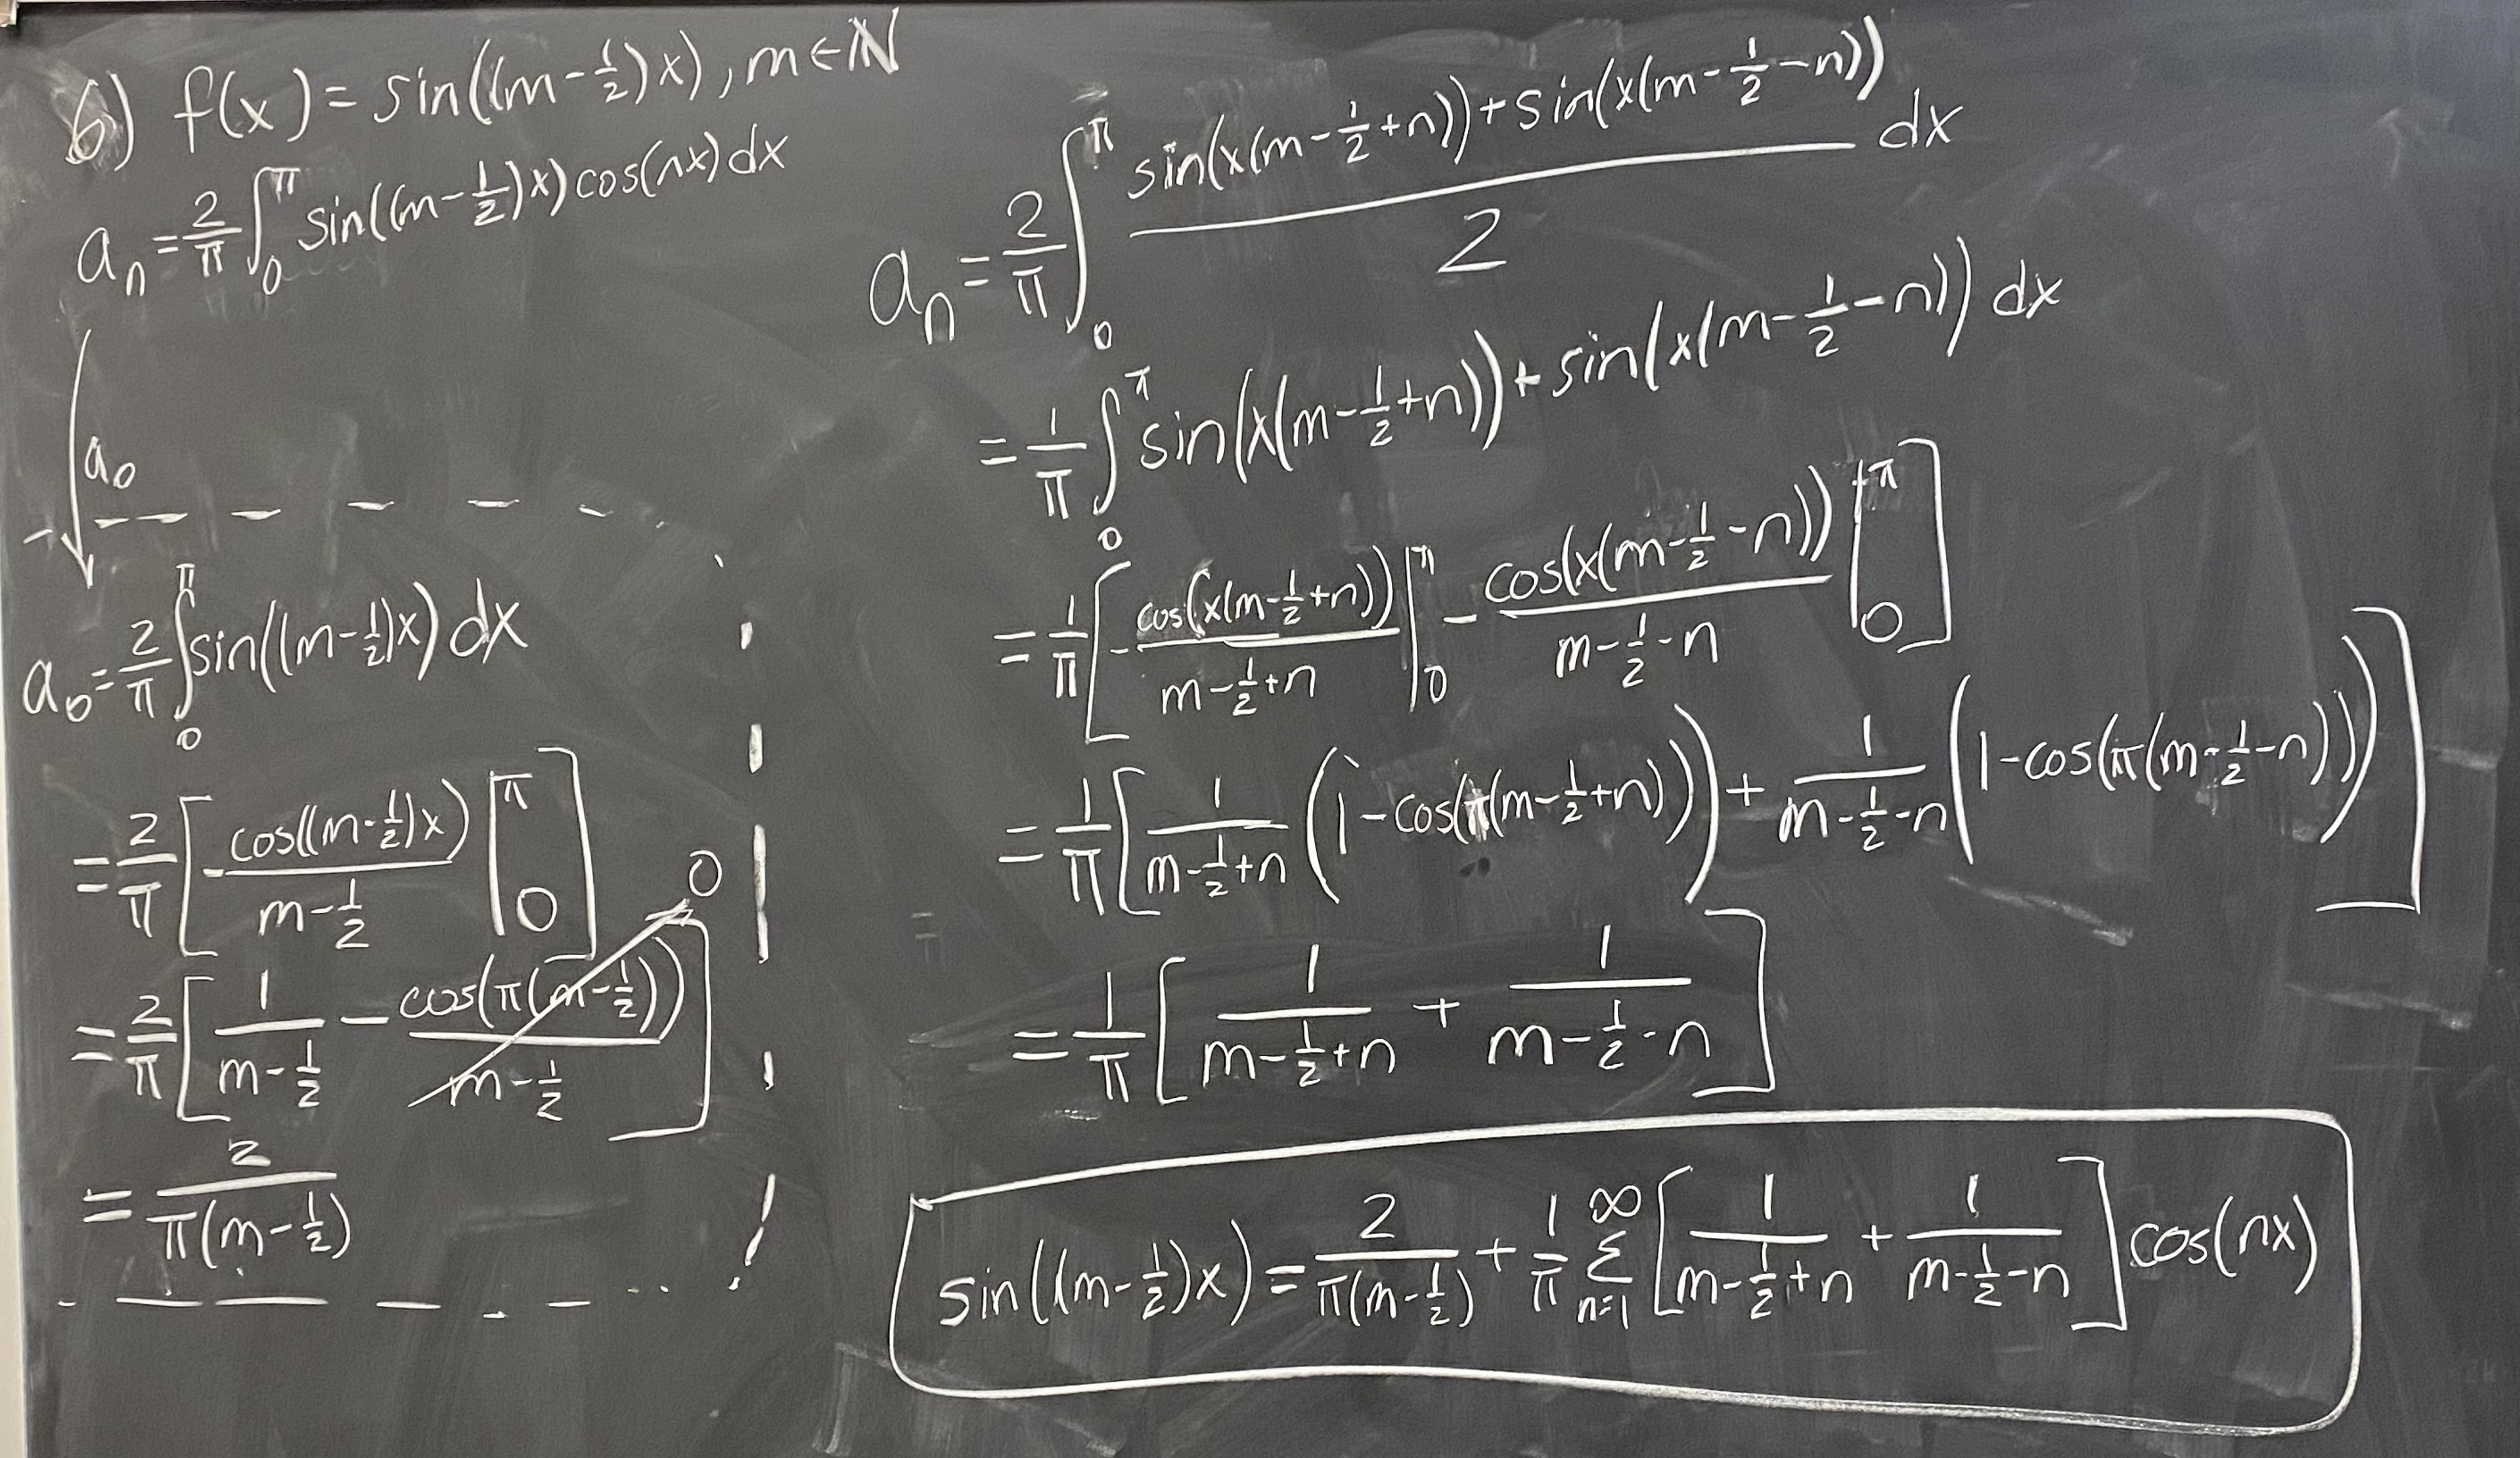
\includegraphics[width = \textwidth]{Problem 5-6.jpg}
        \end{figure}
    \end{enumerate}
\end{ans}

\end{document}
